\documentclass[sigconf,anonymous,review]{acmart}
\usepackage{booktabs}
\usepackage{array}
\usepackage{makecell}
\usepackage{graphicx}
\usepackage{float}
\usepackage{algorithm}
\usepackage[noend]{algpseudocode}
\settopmatter{printacmref=false}
\setcopyright{none}
\renewcommand\footnotetextcopyrightpermission[1]{}
\acmConference[WWW '27]{The ACM Web Conference 2027}{2027}{TBD}
\acmYear{2027}
\acmDOI{}
\acmISBN{}
% Single definition of the anonymous artifact link (placeholder until the anonymous mirror is created).
\providecommand{\anonrepo}{\url{https://anonymous.4open.science/r/freeze-then-certify-ANON}}

\newcommand{\cA}{\mathcal{A}}
\newcommand{\eps}{\varepsilon}
\newcommand{\dmain}{\delta_{\text{main}}}
\newcommand{\dvar}{\delta_{\text{var}}}
\newcommand{\Npen}{N_{80}^{\text{pen}}}
\renewcommand{\thetable}{S\arabic{table}}
\renewcommand{\thefigure}{S\arabic{figure}}
\newcommand{\meff}{m_{\text{eff}}}
\renewcommand{\thesection}{S\arabic{section}}
\begin{document}
\sloppy
\title{Supplementary Material for ``Freeze, Then Certify: Finite-Population Joint Certificates for Budgeted Targeting Policies on Randomized Logs''}
\author{Anonymous Author(s)}
\affiliation{\institution{Anonymous Institution}\country{}}
\maketitle

This supplement holds material moved from the paper to meet the page limit: the earlier confirmatory rounds (S1), the dated deviation table (S2), the Lenta table (S3), the reproducibility record with the implementation checks (S4), the full comparator table of the Criteo test with the trajectory, the plan contrast and the guaranteed-method table (S5), the descriptive blocks of the X5 test with the speed-versus-guarantee figure (S6), the validity argument for the phased joint certificates (S7), the post-hoc adaptive block (S8), what remains untested (S9), the sensitivity block (S10), the semi-synthetic adaptive regime with the equal-information and charged-pilot block F2 (S11), the FDC-HG and FDC-LOC ablations with the dense-monitoring block and every row of the lock-v9 time-uniform test (S12), the three-arm Hillstrom block with its lock-v9 evaluation-half rerun (S13), an errata index for locked files and earlier drafts (S14), a notation glossary (S15), the cost conversion at published list prices with the priced-access workflow (S16), FDC-DP, its proofs and every lock-v10 row (S17), the converse remarks to Proposition 4.3 (S18), the post-hoc block G with its tolerance sweep, knapsack costs and stronger rivals (S19), the localised union ledgers tried on development halves (S20, negative), the lock-v11 confirmatory block on the Open Bandit Dataset (S21), the paragraphs that revision r7 moved out of the paper to make room for it (S22), the lock-v12 descriptive replications on two further Open Bandit campaigns (S23), and the paper's former mechanism and method-glossary tables (S24). Table~\ref{tab:ckpanels} in S1 holds the checkpoint-test rows formerly in Table 1B and 1C of the paper. In the repository (\anonrepo) the Criteo test is lock v7, the X5 test is lock v8 and the time-uniform test is lock v9 (blocks A and B; block C is Hillstrom); the scaling test of Section 6.5 is lock v10, the fresh-log test of Section 6.6 is lock v11, and its two descriptive replications (Section 6.6, S23) are lock v12. Section, table and claim references (C1--C4, Table 1, Theorem 4.1, Remark 4.2, Proposition 4.3, Table A1) point to the main paper.

\section{Earlier confirmatory rounds}\label{app:earlier}

Table~\ref{tab:ckpanels} holds the confirmatory rows of the two checkpoint-strength tests (locks v7 and v8), which the paper's Table 1B now summarises in one row.

\begin{table*}[t]
\caption{\textbf{Checkpoint-strength tests} (moved from Table 1B and 1C of the paper in revision r6; the paper keeps a one-row summary). 200 fresh paired streams per test. Rows = geometric-mean $\Npen$. Ratio = paired geometric mean of FDC-BF / method, 95\% CI and one-sided UB95; Thr.\ = registered threshold (--- = descriptive); F/T/S = \% of streams on which FDC-BF stops earlier / at the same time / later. Guar.: CP = valid at the 20 checkpoints; TU = time-uniform under any predictable sampling (FDC-BF and RECT-ck-BF are also time-uniform on the frozen schedule, Remark 4.2). Every method: 0/200 false streams and 12/15 before $\tau_R$ on every stream. $^\ddagger$Post hoc on the Criteo-test streams. $^\S$More comparators in Table~\ref{tab:fullv7} and S6.}
\label{tab:ckpanels}
\small
\setlength{\tabcolsep}{3.3pt}
\begin{tabular}{@{}lllrlrlrll@{}}
\toprule
Method & Role & Guar. & Rows & FDC-BF / method [95\% CI] & UB95 & Thr. & F / T / S & $x_{12}$ ratio [UB] & $N_{100}$ ratio [UB] \\
\midrule
\multicolumn{10}{@{}l}{\emph{Criteo test (lock v7), 20 checkpoints, seeds 33000--33199, $\eps = 0.001$, rows in millions (FDC-BF: 0.91M)$^\S$}} \\
\textbf{RECT-ck-HG} (exact) and \textbf{-live} & primary & CP & 1.41 & \textbf{0.643} [0.625, 0.661] & \textbf{0.658} & $<$0.80 & 98.5 / 1.5 / 0 & 0.633 [0.644] & 0.687 [0.700] \\
\textbf{HC-WoR} (betting) & primary & TU & 1.39 & \textbf{0.655} [0.639, 0.673] & \textbf{0.670} & $<$0.80 & 99.0 / 1.0 / 0 & 0.649 [0.660] & 0.704 [0.717] \\
PJC-local*$^\ddagger$ & descr. & CP & 0.91 & 1.001 [0.995, 1.008] & 1.007 & --- & 1.5 / 96.5 / 2.0 & 0.999 [1.002] & 1.001 [1.004] \\
PJC-menu*$^\ddagger$ & descr. & CP & 0.93 & 0.976 [0.964, 0.986] & 0.985 & --- & 9.0 / 91 / 0 & 0.965 [0.969] & 0.997 [1.000] \\
RECT-ck-BF (matched)$^\ddagger$ & descr. & CP & 1.82 & 0.498 [0.484, 0.512] & 0.510 & --- & 100 / 0 / 0 & 0.506 [0.516] & 0.581 [0.587] \\
\midrule
\multicolumn{10}{@{}l}{\emph{X5 test (lock v8, first use of the X5 half), 20 checkpoints, seeds 35000--35199, $\eps = 0.02$, rows in thousands (FDC-BF: 24.4k)$^\S$}} \\
\textbf{RECT-ck-HG*} (plan 0.5), \textbf{-live} & primary & CP & 67.1 & \textbf{0.364} [0.358, 0.370] & \textbf{0.368} & $<$0.60 & 100 / 0 / 0 & 0.354 [0.357] & 0.387 [0.393] \\
\textbf{HC-WoR*} (Neyman) & primary & TU & 67.4 & \textbf{0.362} [0.356, 0.368] & \textbf{0.367} & $<$0.60 & 100 / 0 / 0 & 0.352 [0.355] & 0.380 [0.386] \\
\textbf{PJC-local*} (no boundary) & primary & CP & 24.3 & \textbf{1.003} [0.994, 1.012] & \textbf{1.011} & $<$1.05 & 4.5 / 89.5 / 6.0 & 1.005 [1.008] & 0.999 [1.008] \\
\textbf{PJC-menu*} & primary & CP & 25.2 & \textbf{0.968} [0.956, 0.979] & \textbf{0.978} & $<$1.05 & 18 / 80 / 2.0 & 0.969 [0.972] & 0.964 [0.975] \\
RECT-ck-BF (matched) & descr. & CP & 81.6 & 0.299 [0.294, 0.304] & 0.303 & --- & 100 / 0 / 0 & 0.310 [0.313] & 0.335 [0.340] \\
\bottomrule
\end{tabular}
\end{table*}


\textbf{Lock v5 (FDC, seeds 30000--30199).} FDC needed 0.487 [0.472, 0.501] times the rows of the hardest of the nine original rivals (B4-bal; UB95 0.499) with 0/200 false streams, and 1.098 [1.073, 1.127] and 1.084 [1.051, 1.114] times the rows of the tuned plug-in ports FIX-bal-fav and B2-fav-tight. Against B2-fav-tight, FDC stopped earlier on 2 streams, at the same checkpoint on 139 and later on 59. In that table, a ``reached at $\tau_R$'' count of 1 for B2-fav-tight (seed 30039) and for B5 (seed 30149) reflects the failure penalty of a false certificate, not reading the whole half; B3-fav never reached 12 of 15 (0/200). On a finer $K = 60$ grid (100 streams) the ratios against the four closest guaranteed rivals were 0.491--0.554, while against the tuned plug-in port B2-fav-tight FDC needed 1.097 [1.037, 1.146] times the rows and was later on 70\% of streams, and on CR12 ($|\Pi| = 4{,}096$, 50 streams) FDC/B4-bal was 0.570 [0.533, 0.607].

\textbf{Lock v6 (seeds 31000--31199 and continuations of 30000--30199).} Against the same-plan tight rectangles FDC was 0.851 [0.828, 0.875] (RECT-ck-HG; UB95 0.871) and 0.869 [0.847, 0.892] (HC-WoR; UB95 0.888), a preregistered \emph{downgrade}. FDC was later than RECT-ck-HG, RECT-ck-HG-live and HC-WoR on 2 of 200 streams each (seeds 31025 and 31042 against the exact rectangles, 31025 and 31147 against HC-WoR; at seed 31025 FDC read 1,904,850 rows against 1,468,724), and tied on about half. On the full-frontier endpoint, continued from the v5 streams, FDC beat all nine original rivals with UB95 at most 0.613. These rounds explain why FDC-BF exists and are reported here so that the reader sees the full sequence.

\section{Dated deviations}\label{app:deviations}

\begin{table*}[p]
\caption{\textbf{Dated deviations} (lock v5 through lock v12). None changes a locked verdict; each bounds how a result may be worded. The table continues over 4 pages.}
\label{tab:deviations}
\small
\begin{tabular}{@{}l>{\raggedright\arraybackslash}p{6.6cm}>{\raggedright\arraybackslash}p{7.6cm}@{}}
\toprule
When & What & Consequence for this paper \\
\midrule
2026-10-02 & $\eps = 0.001$ set by a guard that read evaluation-half aggregate truth (no evaluation stream) & guard did not bind; the evaluation table is not untouched \\
2026-10-03 & 50/50 share and $\delta$ split 0.045/0.005 chosen after the round-4 results; shares 0.30--0.60 explored on development seeds & forking-path risk; B4-bal's own tuning chose 0.50 \\
2026-10-03 & headline narrowed from ``faster than published plug-in configurations'' to ``faster than guaranteed methods'' (explicit user decision after development data) & plug-in rules descriptive; FDC beat published B2-fav and Peace-fav but not tuned ports \\
2026-10-03 & v5 effect gate relaxed from ratio 0.67 to UB95 $< 1$; non-inferiority to tuned plug-ins demoted to an estimate & v5 results also clear the original gate (UB95 0.499) \\
2026-10-03 & v5 decomposition's frozen prediction model failed (log error 0.264 $>$ 0.095) & decomposition reported as descriptive only \\
2026-10-03 & tuning asymmetry: FDC's development exploration (share, threshold, grid, ledger) exceeded any rival's tuning & mitigated, not removed: exact rectangles have no fitted scalar, but allocation, error-spending and certificate-family choices remain \\
2026-10-03 & v5 replica checker revised (v1 to v2) after a false positive on a summary-only change & 580/580 rerun rows match \\
2026-10-04 & lock v6: FDC downgraded against tight rectangles (UB95 0.888) & reported; motivates FDC-BF \\
2026-10-04 & FDC-BF designed after v6 evaluation results; 18 certificate variants (lock JSON list; lock prose says about 22) compared on development data; chosen by judgement & post-hoc method; only block A of lock v7 is confirmatory \\
2026-10-04 & v7 primary family reduced from four (v6, incl.\ RECT-ck-Bern) to three, declared before any v7 run; rivals not retuned & C2 limited to registered rivals \\
2026-10-04 & near-duplicates found on the v7 streams: RECT-ck-HG-live and RECT-ck-HG have equal $\Npen$ on every stream ($x_{12}$ differs on 6/200); Hait-SW and B4-bal have equal $\Npen$ and $N_{100}$ ($x_{12}$ differs on 200/200, certification checkpoints on 28/200); B2-rect and RECT-ck-Bern differ in $\Npen$ on 2/200 and in $N_{100}$ on 8/200 & reported as fewer distinct constructions on the primary endpoint \\
2026-10-04 (r2) & erratum: v6 FDC was later than each tight rectangle on 2/200 streams (earlier text said never later) & corrected in S1 and in \texttt{v6\_summary.md} \\
2026-10-04 & lock v7 threshold 0.80, looser than v6's 0.70, fixed before any v7 run & observed UB95 0.670 clears both \\
2026-10-04 & one run per method read for $N_{80}$, $x_{12}$, $N_{100}$; false streams counted over the full run & stricter than the stop-at-12 window \\
2026-10-04 & exploration-document errata: FDC-BF is Bennett-FPC only (not Bennett $\wedge$ KL); a dominance remark over fixed-$\lambda$ betting narrowed & code never changed \\
2026-10-04 & lock v8: X5 RetailHero chosen after lock v7 (Criteo has no untouched rows; the local 100k \texttt{criteo\_uplift} file is a synthetic stand-in, never used; MegaFon rejected as synthetic) & second confirmatory table is post hoc in choice, untouched in outcomes \\
2026-10-04 & lock v8: PJC family designed after v7 results, at reviewers' request; no-reset member added before the lock on the code reviewer's advice and selected on X5 and CR9 development data & PJC-local* is non-adaptive; only PJC-menu* adapts; C3 stated as non-inferiority \\
2026-10-04 & lock v8: thresholds 0.60 / 1.05 and decision $\eps = 0.02$ sized from X5 development seeds 900--949; later runner check on 950--999 changed nothing & prospectively locked for evaluation, but selected using development outcomes \\
\bottomrule
\end{tabular}
\end{table*}

\begin{table*}[p]
\addtocounter{table}{-1}
\caption{\textbf{Dated deviations}, continued (part 2 of 4).}
\small
\begin{tabular}{@{}l>{\raggedright\arraybackslash}p{6.6cm}>{\raggedright\arraybackslash}p{7.6cm}@{}}
\toprule
When & What & Consequence for this paper \\
\midrule
2026-10-04 & lock v8: X5 blinding procedural (raw outcomes kept; ingest wrote evaluation outcomes unreduced; hashes read bytes; no statistic computed) & cannot be verified beyond code and git history \\
2026-10-04 & lock v8: PJC phase plans take effect at the next replanning batch after the boundary, registered as implemented & validity unaffected; tuning used the same behaviour \\
2026-10-04 & lock v8: v6\_summary.md erratum (bound by v7) accepted as the only input drift; gate chain does not re-verify the v5 lock's own input manifest & inherited scope limit, no v8 computation depends on it \\
2026-10-04 & lock v8: PJC-menu* chose the 50/50 menu item on all 200 X5 streams & its 3\% deficit reflects its larger union (37 instead of 20 events per direction, in both exponent and variance level) and deterministic tracking, not separated; the registered test did not exercise adaptation \\
2026-10-04 (r3) & post-hoc adaptive block (S8) run after lock v8 at a reviewer's request; members, grid and dev-tuning rule fixed before any of its evaluation rows; evaluation access through a logged post-hoc path & descriptive only; cannot change C3, which remains the registered non-inferiority result \\
2026-10-04 (r3) & width proposition (Prop.~4.3) and its development-data predictions derived after the observed ratios were known & descriptive account of the mechanism; no threshold or claim depends on it \\
2026-10-04 (r3) & mechanism table rebuilt on the matched rectangle; the earlier ``FPC / no FPC'' row (exact HG vs Bernstein, interaction 0.285) relabelled as not an aggregation contrast; Criteo RECT-ck-BF rows corrected from 1.83M to 1.82M & matched interaction 0.030 [$-$0.001, 0.060] \\
2026-10-04 (r4) & FDC-HG (exact-HG cell envelope) designed after lock v8 at the authors' initiative; go criteria fixed in \texttt{plan/v9\_plan.md} before its development runs; no-go & reported as a descriptive ablation (S12) \\
2026-10-04 (r4) & FDC-LOC (gap-localised union) and the time-uniform extension stated with go criteria before any run (commit \texttt{61ce3930}); FDC-LOC no-go, time-uniform go & Remark 4.2 is a post-hoc theoretical observation; the checkpoint procedure is unchanged and its numbers are identical only when evaluated on the $K = 20$ grid; lock v9's dense monitoring can change stopping times (row 2026-10-05 below) \\
2026-10-04 (r4) & sensitivity block (S10) and semi-synthetic regime block (S11) run on development halves after the r3 revision, at reviewers' request; knob values and regimes fixed before their rows & descriptive; cannot change C2 or C3 \\
2026-10-04 (r4) & Hillstrom design rule revised twice (v1 voided, v2 = design A with every rival at $\tau_R$, rule B = design B) on the development half; design B relies on an unsourced half price for the women's e-mail & descriptive only (S13); lock-v9 block C registered as a descriptive reuse \\
2026-10-04 (r4) & hypothetical unit prices of the then Table 2 (now Table~\ref{tab:cost}) replaced by published list prices of analogous services & still a conversion, not a measured bill \\
2026-10-05 & lock v9: the time-uniform reading of FDC-BF (TU-FDC; Theorem TU-1 in \texttt{plan/v9\_candidates\_theory.md}) found after the lock-v8 results; the formerly secondary 77-time dense design promoted to primary; TU-FDC evaluated through a new wrapper that can change stopping times relative to 20-checkpoint FDC-BF & post-hoc reading of an unchanged procedure (identical to FDC-BF on the 20-point grid), disclosed as a change of confirmatory design \\
\bottomrule
\end{tabular}
\end{table*}

\begin{table*}[p]
\addtocounter{table}{-1}
\caption{\textbf{Dated deviations}, continued (part 3 of 4).}
\small
\begin{tabular}{@{}l>{\raggedright\arraybackslash}p{6.6cm}>{\raggedright\arraybackslash}p{7.6cm}@{}}
\toprule
When & What & Consequence for this paper \\
\midrule
2026-10-05 & lock v9: RECT-ck-BF-TU built for this lock (RECT-ck-BF+box with radii frozen at the last checkpoint, no tuning parameter); TU-PJC registered as a second non-inferiority rival after an external review (r1 P1), because PJC-local* with a 77-time ledger has a cost that is not predetermined & rectangle claim covers only the two registered constructions; non-inferiority worded ``matches PJC'', never ``faster than PJC'' \\
2026-10-05 & lock v9: thresholds 0.85 (Criteo) and 0.50 (X5) sized from development dense-grid ratios 0.708 (UB95 0.737) and 0.356 (UB95 0.365); inherited 1.05 margin had 0.034 of development headroom against TU-PJC & observed UB95 0.723, 0.379 and non-inferiority 1.009 \\
2026-10-05 & lock v9: table reuse, the fourth fresh-stream use of the Criteo evaluation half and the second of the X5 half; only the seeds are new & confirmation conditional on the two finite tables, not replication across populations \\
2026-10-05 & lock v9: FDC-HG and FDC-LOC (no-go) entered only as descriptive rows; the invalid dense control had 0/200 false streams on the toy & ablation rows descriptive; dense validity rests on the proof, not on the toy \\
2026-10-05 & lock v9 block C: Hillstrom evaluation half rerun as a preregistered descriptive reuse of an outcome-exposed log (designs B and A) & wording rule only; no verdict, never merged with blocks A and B \\
2026-10-05 (r5) & block F2 (equal pilot information and charged pilot reads for the semi-synthetic regimes of S11) run after block F's results, in response to a reviewer; pilot sizes, charging rule, amortisation grid and the adaptive picks' pilot initialisation fixed before any F2 row; adaptive picks not retuned with a pilot & post hoc, semi-synthetic, descriptive; supports the new C3 only in the qualified form of S11 \\
2026-10-05 (r5) & claim C3 redefined: the registered PJC non-inferiority result (C3 in earlier rows) becomes a supporting result of Section 6.3, and C3 is now the post-hoc allocation claim of block F2 & earlier rows' ``C3'' refer to the non-inferiority result; the post-hoc C3 carries no confirmatory weight \\
2026-10-05 (v10) & FDC-DP designed after lock v9 to scale the certificate to implicit classes; go criteria fixed before its development runs; each cell's $\eps$ chosen on development data by a rival-success rule written before the $\eps \ge 0.03$ runs; v1 development numbers superseded after an external code review (weighted centre, stop at 15 of 15, exactness contract) & computational contribution only; development endpoints reproduce; $\eps$ varies with $S$, so the cells are not a controlled scaling experiment (S17) \\
2026-10-05 (v10) & table reuse: X5 evaluation half in its third use; Lenta LR9 evaluation half in its third fresh-stream use and first confirmatory use, outcome-exposed; HC-WoR-DP an untuned nine-segment transfer; X5 at $S = 64$ descriptive (no qualifying $\eps$); Lenta comparisons exhaustion-sensitive & claims restricted to the named rectangles on these finite tables; Lenta $S = 16$ gain exhaustion-assisted (S17) \\
2026-10-05 (r5) & lock-v10 results integrated: FDC-DP added as a contribution under C1 (validity) and C2 (confirmatory evidence), keeping four claims & both v10 blocks positive; scalability limit of earlier drafts replaced by the cardinality-budget scope \\
2026-10-05 (r6) & lock-v10 reading: the development $\eps$ rule places RECT-BF-DP-TU at checkpoint 19 of 20 on every stream of four cells and 197 of 200 of the fifth; Lenta's pre-exhaustion width claim withdrawn (the lock permits it only where both exhaustion fractions are zero) & ratios are FDC-DP's stopping point over a fixed rival reading; verdicts unchanged; reads-versus-$\eps$ curves added (block G, post hoc, \S\ref{app:blockg}) \\
\bottomrule
\end{tabular}
\end{table*}

\begin{table*}[p]
\addtocounter{table}{-1}
\caption{\textbf{Dated deviations}, continued (part 4 of 4).}
\small
\begin{tabular}{@{}l>{\raggedright\arraybackslash}p{6.6cm}>{\raggedright\arraybackslash}p{7.6cm}@{}}
\toprule
When & What & Consequence for this paper \\
\midrule
2026-10-05 (r6) & wording corrections after the r5 reviews: FDC-DP evaluates FDC-BF's certificate family on a global $\lambda$ grid (not the same certificate); DP pseudo-polynomial, branch-and-bound exact on its grid but exponential in the worst case; matched rectangle described as a construction comparison with clipping and intersections; pilot comparisons separated; read-saving percentages recomputed as $1 - 1/r$ & no number or verdict changed; checked by \texttt{verify\_r6\_numbers.py} \\
2026-10-05 (v11) & lock v11: a never-replayed randomized log (Open Bandit Dataset, \texttt{random/all}) added after the r6c reviews to answer the reuse objection; arm groups (top 40 items by development click rate) and the uf0 $\times$ uf3 segmentation chosen with development outcomes; $K$ raised from 20 to 40 (pre-stated in the plan); costs frozen from development traffic shares; $\eps$ and THRESH from pre-stated development rules; development block regenerated once after the first external lock review (no stream computation changed) & disclosed in Section 7 of the paper and S21; claims limited to the named rectangles on this one log \\
2026-10-05 (r7) & lock-v11 results integrated: C2 extended to the fresh log; Figure 2 and several Section 6 paragraphs moved to S19 and S22 for space & no number changed; moved text verbatim in S22 \\
2026-10-05 (r7b) & lock-v11 reporting corrected after the r7 reviews: the r7 claim that v11 meets the lock-v10 pre-exhaustion condition withdrawn (the rival reaches $\tau_R$ on 12 of 200 streams); stopping fractions and the ``last eighth'' sentence corrected; uncensored-subset (0.821) and full-frontier (0.853) ratios added as descriptive; scope sentences of the paper, S9, S20 and S22 narrowed & verdict and every registered number unchanged; S14 lists the errata \\
2026-10-05 (v12) & lock v12: lock-v11 protocol replicated on \texttt{random/women} and \texttt{random/men} (fresh salted splits, rules re-derived on each development half); a block-status gate written in the plan before any split made both blocks descriptive ($\eps$-optimal development share 0.661 and 0.858 $> 0.5$ at the rule-selected $\eps = 7.5\cdot 10^{-4}$ and $10^{-3}$); descriptive-block output relabelled (no verdict, THRESH not applicable) after the gate result and the development block regenerated once (4,980 rows identical); unsaved pre-rule smoke streams; external review round 2 ``fix-then-lock'' with two P2 wording residues fixed before the lock & no confirmatory claim; reported in Section 6.6 and S23 as descriptive replication evidence, never pooled with lock v11; the fresh-log part of C2 rests on lock v11 alone \\
2026-10-05 (r8) & lock-v12 results integrated: one paragraph in Section 6.6 and one sentence in Section 7; paid for by shortening Sections 5, 6.2--6.5 and 6.7 to sentences already in S16, S17 and S22 & no earlier number or verdict changed; checked by \texttt{verify\_r8\_numbers.py} \\
2026-10-06 (r9) & after an independent review of r8d: the certified estimand (the observed-pool objective a full-log analysis computes) and the 12-of-15 endpoint stated in the abstract and Sections 1--2; the Open Bandit full-frontier ratio (S21) brought into Section 6.6; a post-hoc decision-difficulty census of every block added (S25, Table 3 of the paper); history paragraphs of Sections 5--7 shortened to sentences kept here and in S12--S23; this table split across pages & no registered number or verdict changed; the X5 and Lenta scaling frontiers are reported as near-trivial at their tolerances \\
by design & guarantee strength: FDC-BF checkpoint-valid and, under the frozen plan, time-uniform (Remark 4.2); HC-WoR and WSR20 rectangles time-uniform under any predictable sampling & the time-uniform test (lock v9) matches strength on the frozen plan; HC-WoR remains valid under adaptive sampling, which no comparison uses \\
\bottomrule
\end{tabular}
\end{table*}

Table~\ref{tab:deviations} lists every departure we know of, from the choice of $\eps$ to the selection of FDC-BF and the later errata; errata to locked files and earlier drafts are indexed in S14. The full machine-readable log, including rationale, decision maker and evidence path for each entry, is in the anonymous repository.

\section{Lenta (descriptive)}\label{app:lenta}

\begin{table}[H]
\caption{\textbf{Lenta LR9, lock v7 block B} (200 streams, seeds 34000--34199; outcome-exposed reuse, no decision rule). Paired $\Npen$ ratios FDC-BF / method [95\% CI]; last rows: geometric-mean $\Npen/\tau_R$ (\% of streams at $\tau_R$). All methods: 0 false streams.}
\label{tab:lenta}
\footnotesize
\setlength{\tabcolsep}{2pt}
\begin{tabular}{@{}llll@{}}
\toprule
Method & $\eps = 0.002$ & $\eps = 0.003$ & $\eps = 0.004$ \\
\midrule
RECT-ck-HG & 0.798 [0.791, 0.805] & 0.672 [0.664, 0.680] & 0.676 [0.666, 0.686] \\
RECT-ck-HG-live & 0.803 [0.798, 0.808] & 0.701 [0.691, 0.711] & 0.678 [0.668, 0.688] \\
HC-WoR & 0.717 [0.706, 0.728] & 0.668 [0.660, 0.677] & 0.674 [0.665, 0.684] \\
FDC (v5) & 0.646 [0.642, 0.649] & 0.785 [0.776, 0.795] & 0.802 [0.790, 0.815] \\
other guaranteed$^\dagger$ & 0.646 & 0.524 & 0.433--0.434 \\
\midrule
FDC-BF $N/\tau_R$ & 0.646 (0\%) & 0.524 (0\%) & 0.433 (0\%) \\
RECT-ck-HG & 0.809 (5\%) & 0.779 (0\%) & 0.641 (0\%) \\
HC-WoR & 0.901 (53\%) & 0.784 (0\%) & 0.643 (0\%) \\
FDC (v5) & 1.000 (100\%) & 0.667 (0\%) & 0.540 (0\%) \\
\bottomrule
\end{tabular}
\\[2pt]\parbox{\columnwidth}{\footnotesize $^\dagger$B4-bal (share 0.4), QFC-pool, B2-rect, Peace-rect, Hait-SW, RECT-ck-Bern; these reach 12/15 only at $\tau_R$ on 99--100\% of streams, so their ratios are end-point ratios.}
\end{table}

Lenta's evaluation half (343,513 rows, outcome \texttt{response\_att}) was split with a new seed and segmented by age tertile $\times$ promotion-share level, but an earlier analysis had computed cell means on the full table, so no split can restore an untouched holdout. At $\eps \ge 0.003$ all 15 problems are easy and several rivals pile up at $\tau_R$, so only the ratios against the tight rectangles are speed ratios. The multi-resolution variant was 1.12--1.15 times slower than FDC-BF here, as on development data. Lenta therefore supports the ordering of C2 without replicating it.

\section{Reproducibility}\label{app:repro}

Checkpoint grid (paper Section 2): the $K = 20$ checkpoints are log-spaced from 50,000 rows on Criteo (2,000 on X5) to $\tau_R$, so consecutive checkpoints differ by a factor of 1.297 on Criteo and 1.229 on X5; RECT-ck-HG has a live-cell variant (S5).

{\sloppy Locks: v5 sha256 \texttt{64196b5a\ldots6948}; v6 addendum \texttt{9c8dc944\ldots d497}; v7 addendum \texttt{47e195f0\ldots c68f} (code freeze commit \texttt{bfd929bd}, lock commit \texttt{23f7f5e5}). The v7 gate re-verifies the v5 and v6 locks, code, inputs and raw data on every run and refuses a lock file with more than one commit. Seeds: v5 30000--30199, v6 31000--31199 (Criteo) and 32000--32199 (Lenta), v7 33000--33199 (Criteo) and 34000--34199 (Lenta); development 900--999. Each v7 evaluation task wrote a seal (row-content hash, coverage, code, data and lock hashes) committed alone and referenced from a second single commit; seal commits \texttt{53133736}, \texttt{a4305d20} (block A) and \texttt{8dd4abde}, \texttt{cd61d569} (block B). Replica: a separate process running the same code reran the first 10 seeds of each task with identical rows (R1), and all 50/50 methods had identical schedule digests on every stream (R2); both passed for all four tasks. Cost: block A took 30.5 + 34.4 wall-clock minutes (15,473 CPU-seconds). Certificate cost: about 0.1\,s per checkpoint and 1.3\,s per stream, 59\% of the replay engine's compute time (\texttt{rs\_sec\_cert}/\texttt{rs\_sec\_total} in the sealed rows). An external code review found no validity bug in FDC-BF and three lock gaps (resealing, a missing history anchor for the lock, inconsistent disclosure wording), all fixed before locking. The unmatched contrasts of Table~\ref{tab:mechanism} (S24; formerly main-paper Table A2) are recomputed by \texttt{exp/code/run\_v7\_posthoc\_2x2.py} from the sealed rows and reproduce the lock's bootstrap exactly; the matched contrast (0.739, interaction 0.030), the reads saved in Table~\ref{tab:cost}, and the trajectory medians are recomputed from the sealed rows by \texttt{writing/scripts/verify\_r3\_numbers.py}. The headline method is the factory entry \texttt{FDCBet(kind="bennett")}; the class's default \texttt{kind="min"} is not the evaluated variant. Lock v8: addendum sha256 \texttt{729bdcbd\ldots a1cff0} (code freeze commit \texttt{5de13da1}, lock commit \texttt{d568af38}); seeds 35000--35199 (X5, block A), 35200--35399 (CR12, block B), and the v7 seeds 33000--33199 (block C); X5 development seeds 900--999. Seal commits \texttt{737566cb}, \texttt{853ef8cb} (block A), \texttt{9a4414d8}, \texttt{0830286d} (block B), \texttt{33953104} (block C). Replicas R1 (first 10 seeds rerun in a separate process), R2 (schedule digests within each design group) and R2b (identical arrival sequences across all methods of a stream, also across tasks) passed for all five tasks. The v8 gate re-verifies the v7, v6 and v5 locks on every run. An external code review (two rounds) found one blocking issue (cross-task R2b not entering the replica status) and five major ones (hash of the consumed schedule, missing no-reset PJC member, phase activation, unbound lock text and provenance file, over-strong blinding wording), all resolved before the lock.\par}


\textbf{Implementation checks.} Numerical MGF domination of Lemma A.1 for $N \in \{10, 23, 40, 101\}$, six sample sizes, all $M$ and 50 arguments (maximum violation $\le 10^{-9}$); Monte Carlo tails of four-cell directions at a loose test level $\beta = \ln 8$ (nominal tail 0.125; the operational level $e^{-\beta} \approx 6.6 \times 10^{-7}$ is covered by the proof, not by simulation); correctness of the box supremum; agreement of a re-implementation of FDC with the original (statistics equal to relative tolerance $10^{-9}$; certification checkpoints, answers and schedule digests identical); exact ledger $\dmain$; and, on the toy harness used to explore FDC-BF's design, an invalid naive joint certificate produced 5 familywise errors while every valid variant produced none. For FDC, 60 synthetic finite-pool configurations gave 0 false certifications in 1,350,000 and no miss of either event over 118,320,000 audited events. For the time-uniform extension (Remark 4.2), a single-cell Monte Carlo test ($N = 300$, $M = 90$, $n_0 = 30$, 6,000 permutations, level 0.10) gave a crossing frequency over all $n \ge n_0$ of 0.036, against 0.553 for an invalid control that refreshes a fixed-$n$ quantile at every $n$, and on a near-tie toy monitored at 77 times FDC-BF with stale widths had 0/200 false streams against 6/200 for an invalid naive joint certificate. Every number added in revision r4 is recomputed from result files by \texttt{writing/scripts/verify\_r4\_numbers.py} and \texttt{verify\_r4b\_numbers.py}, every number added or reworded in revision r5 by \texttt{verify\_r5\_numbers.py} and \texttt{verify\_r5b\_numbers.py}, and every number added or reworded in revision r6 by \texttt{verify\_r6\_numbers.py}; the r4 and r5 supplement tables are generated from result files by \texttt{gen\_r4\_supp\_tables.py} and \texttt{gen\_r5\_supp\_tables.py}.

\textbf{Usage contract for the checkpoint API.} The lock-bound class \texttt{FDCBet} (\texttt{dsswm/baselines/fdc\_bet.py}, hashed by locks v7--v10 and therefore unchanged) computes fresh variance boxes and fresh widths whenever its \texttt{certify} method is called, and checks only that times do not decrease. Its ledger counts exactly the $K$ predeclared checkpoints, so arbitrary increasing times do not authorise fresh widths: a certificate issued between checkpoints with fresh widths is an event the $K$-event ledger never paid for. Revision r6c adds the public entry point \texttt{dsswm/baselines/fdc\_bet\_guarded.py} (\texttt{FDCBetGuarded}, \texttt{make\_guarded\_variant}), which certifies only at the predeclared checkpoints in strictly increasing order, raises \texttt{OffGridCertifyError} otherwise, and is identical to \texttt{FDCBet} on the grid (test \texttt{test\_fdc\_bet\_guarded.py}, four tests). Dense monitoring must use \texttt{FDCTimeUniform} (\texttt{fdc\_loc.py}), which refreshes widths only at block points and reuses the last block's widths in between, as Remark 4.2 requires; the implicit-class certificates \texttt{FDCDP} and \texttt{RectBFDP} already carry the same guard. Every evaluated FDC-BF row was produced on the checkpoint grid or through \texttt{FDCTimeUniform}, so the contract changes no result.

\clearpage
\section{Lock v7: all comparators, trajectory and plan contrast}\label{app:v7full}



\begin{table*}[t]
\caption{\textbf{All lock-v7 comparators, Criteo CR9} (block A; 200 fresh paired streams, seeds 33000--33199, $\eps = 0.001$; the primary rows repeat Table 1B of the paper). Rows = geometric-mean $\Npen$ (millions). Ratio = paired geometric mean of FDC-BF / method with two-sided 95\% CI and one-sided UB95; $<1$ means FDC-BF reads fewer rows. Faster/tied = \% of streams on which FDC-BF stops at an earlier / the same checkpoint (FDC-BF is never later against any listed comparator; it is later than FDC-MR on 16.5\%). ``At $\tau_R$'' = \% of streams that reach 12/15 only after reading the whole half (no stream was penalized for a false certificate). Guarantee: CP = valid at the $K$ pre-specified checkpoints; TU = time-uniform per cell. Every method has 0/200 false streams (Clopper--Pearson UB 0.015). $x_{12}$ and $N_{100}$ columns give the ratio [UB95] on the secondary endpoints. Bold rows form the preregistered primary family; the ten rows below FDC are the comparators omitted from Table 1B.}
\label{tab:fullv7}
\small
\setlength{\tabcolsep}{3.4pt}
\begin{tabular}{@{}lllrlrrrll@{}}
\toprule
Method & Plan & Guar. & Rows & FDC-BF / method [95\% CI] & UB95 & Faster / tied & At $\tau_R$ & $x_{12}$ ratio [UB] & $N_{100}$ ratio [UB] \\
\midrule
FDC-BF (ours) & frozen 50/50 & CP & 0.91 & --- & --- & --- & 0 & --- & --- \\
\textbf{RECT-ck-HG} & frozen 50/50 & CP & 1.41 & \textbf{0.643} [0.625, 0.661] & \textbf{0.658} & 98.5 / 1.5 & 0 & 0.633 [0.644] & 0.687 [0.700] \\
\textbf{RECT-ck-HG-live} & frozen 50/50 & CP & 1.41 & \textbf{0.643} [0.625, 0.661] & \textbf{0.658} & 98.5 / 1.5 & 0 & 0.633 [0.644] & 0.687 [0.700] \\
\textbf{HC-WoR} & frozen 50/50 & TU & 1.39 & \textbf{0.655} [0.639, 0.673] & \textbf{0.670} & 99.0 / 1.0 & 0 & 0.649 [0.660] & 0.704 [0.717] \\
FDC (Bernstein; v5) & frozen 50/50 & CP & 1.19 & 0.761 [0.743, 0.780] & 0.777 & 83.5 / 16.5 & 0 & 0.758 [0.769] & 0.734 [0.745] \\
RECT-ck-Bern & frozen 50/50 & CP & 2.47 & 0.368 [0.357, 0.380] & 0.378 & 100 / 0 & 0 & 0.386 [0.395] & 0.448 [0.452] \\
B4-bal & frozen 50/50 & TU & 2.46 & 0.369 [0.358, 0.380] & 0.379 & 100 / 0 & 0 & 0.371 [0.378] & 0.444 [0.450] \\
Hait-SW & predictable & TU & 2.46 & 0.369 [0.358, 0.380] & 0.379 & 100 / 0 & 0 & 0.370 [0.377] & 0.444 [0.450] \\
B2-rect & adaptive & TU & 2.47 & 0.368 [0.357, 0.380] & 0.378 & 100 / 0 & 0 & 0.366 [0.374] & 0.443 [0.448] \\
QFC-pool & frozen 85/15 & CP & 2.54 & 0.358 [0.346, 0.371] & 0.368 & 100 / 0 & 0 & 0.361 [0.370] & 0.345 [0.349] \\
Peace-rect & adaptive & TU & 2.59 & 0.351 [0.336, 0.366] & 0.363 & 100 / 0 & 3.5 & 0.348 [0.360] & 0.420 [0.432] \\
B3-rect & phased & TU & 3.40 & 0.268 [0.249, 0.287] & 0.284 & 100 / 0 & 30.5 & 0.258 [0.276] & 0.319 [0.338] \\
B1 & adaptive & TU & 3.84 & 0.237 [0.229, 0.244] & 0.243 & 100 / 0 & 0 & 0.237 [0.242] & 0.250 [0.255] \\
B4 & frozen 85/15 & TU & 5.46 & 0.166 [0.162, 0.172] & 0.171 & 100 / 0 & 14.5 & 0.159 [0.163] & 0.176 [0.179] \\
Molitor-WoR & frozen 85/15 & TU & 6.99 & 0.130 [0.126, 0.134] & 0.133 & 100 / 0 & 100 & 0.113 [0.115] & 0.158 [0.160] \\
\midrule
\multicolumn{10}{@{}p{0.98\textwidth}@{}}{\emph{Registered secondary method (same frozen-design certificate family, descriptive):} FDC-MR[front3], a multi-resolution union on the same plan, CP, 0/200 false streams, 0.88M rows; FDC-BF / FDC-MR = 1.034 [1.017, 1.052], UB95 1.049: FDC-BF is earlier on 3.5\%, tied on 80\% and later on 16.5\% of streams, and equal on $N_{100}$ (1.000).} \\
\bottomrule
\end{tabular}
\end{table*}

\begin{figure}[H]
\centering
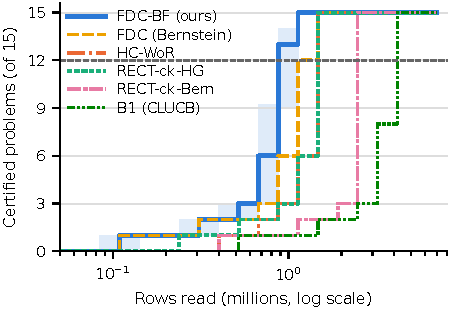
\includegraphics[width=\columnwidth]{../latex_acm/figures/fig2_trajectory_v7.pdf}
\caption{\textbf{Certification trajectory} (Criteo, lock v7 block A). Median certified problems over 200 streams against rows read; the band is FDC-BF's interquartile range and the dashed line the 12/15 endpoint. FDC-BF's median is at least every listed method's at every checkpoint (also at least FDC-MR's). HC-WoR's median coincides with RECT-ck-HG's near the 12/15 endpoint and is one problem lower at three earlier checkpoints (0.24M, 0.31M, 0.52M rows). Medians computed from the sealed rows' certification curves.}
\label{fig:trajectory}
\Description{Step curves of median certified problems against rows read on a log axis for FDC-BF, FDC, HC-WoR, RECT-ck-HG, RECT-ck-Bern and B1; FDC-BF rises first and reaches 15 earliest.}
\end{figure}

\begin{table}[H]
\caption{\textbf{Plan $\times$ aggregation} (Criteo, lock-v5 streams, post hoc; both plans frozen). Rectangles use WSR20 sequences and joint cells are Bernstein joint certificates of the earlier QFC family (the 50/50 one is an intermediate variant, 1.27M; FDC itself read 1.20M). Cells: geometric-mean $\Npen$ (M rows); margins: paired ratios with 95\% CI. $I$: log interaction.}
\label{tab:plan}
\footnotesize
\setlength{\tabcolsep}{3pt}
\begin{tabular}{@{}llll@{}}
\toprule
Plan & Rect.\ (WSR20) & Joint & Joint / rect. \\
\midrule
Log ratio 85/15 & 5.39 (B4) & 2.49 (QFC) & \makecell[l]{0.462\\{}[0.448, 0.476]} \\
Balanced 50/50 & 2.47 (B4-bal) & 1.27 (QFC-50/50) & \makecell[l]{0.514\\{}[0.499, 0.529]} \\
50/50 / 85/15 & \makecell[l]{0.458\\{}[0.451, 0.465]} & \makecell[l]{0.509\\{}[0.492, 0.527]} & \makecell[l]{$I$ = 0.107\\{}[0.072, 0.142]} \\
\bottomrule
\end{tabular}
\end{table}

\textbf{Guaranteed methods and the history of the primary family.} Table~\ref{tab:rivals} lists every guaranteed method with its construction, plan, certificate, tuning and frozen configuration (Table~\ref{tab:glossary} in S24 is a short glossary of the same names). The earlier round's lock fixed a four-member primary family before any of its evaluation runs (the three rectangles above plus RECT-ck-Bern); the Criteo test kept three of them, before any of its runs, as the tightest same-plan rectangles we had constructed: two exact checkpoint rectangles, which have exactly FDC-BF's guarantee strength, and one time-uniform betting rectangle, whose guarantee is stronger in that it holds under any predictable sampling rule; on the frozen schedule FDC-BF is also time-uniform (Remark 4.2). The betting rectangle's inversion was corrected before that lock after an external reviewer found a counterexample that made it looser, never under-covering; on the toy harness used to qualify rivals, all ten rigorous configurations had 0/200 false streams while an invalid naive control had 4/200. Excluded methods, with reasons: B2, B3 and Peace with nominal thresholds and Hait's pooled sequence are proven only for sampling with replacement; Shekhar and Howard (2026) certify a fixed catalogue from a fixed sample; model-internal certifiers are valid only inside a parametric class. Main-paper references give the full citations. A one-cell example shows why fixed-count bounds fail when counts adapt to outcomes within a block: stopping when a fixed-count bound is crossed gave a crossing rate of 0.0845 against the nominal $e^{-3} = 0.0498$. The adaptive ports keep their sampling rules but replan in batches and certify with WSR20 rectangles, so they test valid adaptations, not the original methods; Molitor-WoR keeps per-policy intervals and so does not cancel segments shared by challenger and centre.

\begin{table*}[t]
\caption{\textbf{Guaranteed methods.} Every member carries a proof covering without-replacement replay, its own count rule, checkpoint stopping and one $\delta$ over 15 problems. WSR20 rectangle = per-cell without-replacement confidence sequences (Waudby-Smith and Ramdas, 2020) at level $\delta/(SA)$, combined as a radius sum. Tuning used development seeds 900--949 and the smallest geometric-mean $\Npen$. Adaptive methods replan in batches of $\max(200,\lceil\tau_R/2000\rceil)$ arrivals.}
\label{tab:rivals}
\small
\begin{tabular}{@{}l>{\raggedright\arraybackslash}p{4.0cm}>{\raggedright\arraybackslash}p{2.1cm}>{\raggedright\arraybackslash}p{3.3cm}>{\raggedright\arraybackslash}p{2.5cm}>{\raggedright\arraybackslash}p{2.0cm}@{}}
\toprule
Method & Source / construction & Plan & Certificate & Tuning & Frozen config \\
\midrule
RECT-ck-HG & exact hypergeometric test inversion per (cell, checkpoint) & frozen 50/50 & rectangle, checkpoint-valid, $\alpha = 0.05/720$ & none & --- \\
RECT-ck-HG-live & as above, level $\delta/K$ per checkpoint shared among live cells & frozen 50/50 & rectangle, checkpoint-valid & none & --- \\
HC-WoR & hedged-capital WoR betting CS & frozen 50/50 & rectangle, time-uniform, $\delta/18$ per cell & 6-point grid & $n^*$-scaled, $c = 0.75$, $t^* = 0.2$ \\
RECT-ck-Bern & FDC's Bernstein lemma per cell & frozen 50/50 & rectangle, checkpoint-valid, split 0.045/0.005 & none & --- \\
FDC & Bernstein joint certificate & frozen 50/50 & joint, checkpoint-valid & none at lock & --- \\
B4-bal & balanced design & frozen 50/50 & WSR20 rectangle & share $\in$ \{0.40, 0.45, 0.50\} & 0.50 \\
B4 & log's assignment ratio & frozen 85/15 & WSR20 rectangle & none & --- \\
B1 & CLUCB (Chen et al., 2014) & adaptive & WSR20 rectangle & none & published \\
B2-rect & CombGame (Jourdan et al., 2021) & adaptive & WSR20 rectangle & exploration $\in$ \{1, 0.5\} & 1.0 \\
B3-rect & RAGE (Fiez et al., 2019) & phased & WSR20 rectangle & none & published \\
Peace-rect & Peace (Katz-Samuels et al., 2020) & adaptive & WSR20 rectangle & none & published \\
Hait-SW & layered design (Hait, 2026) & predictable plug-in & WSR20 local sequences & $p_{\min} \times \gamma$ (6) & 0.02, 2/3 \\
Molitor-WoR & per-policy elimination (Molitor, 2026) & frozen 85/15 & per-policy sequences & none & published \\
QFC-pool & earlier unpublished variant of FDC (this study) & frozen 85/15 & joint, checkpoint-valid & none & earlier ledger \\
\midrule
\multicolumn{6}{@{}l}{\emph{X5 test (tuned on X5 development seeds 900--949 at $\eps = 0.02$, argmin geometric-mean $\Npen$ with 0 false streams; RECT-ck-HG-live untuned)}} \\
RECT-ck-HG* & as above, own frozen plan & 50/50 (of 7 plans) & rectangle, checkpoint-valid & plan $\in$ \{0.3--0.7, Neyman, sd$^{2/3}$\} & plan 0.5 \\
HC-WoR* & as above, own frozen plan & Neyman (dev variances) & rectangle, time-uniform & 9 schedules $\times$ 7 plans & $n^*$, $c = 0.75$, target 0.6 \\
PJC-local* & phased joint certificate, RAGE-style phases, residual-pool estimator & deterministic tracking & joint, FDC-BF width and ledger & 17 configs (boundaries, rule) & no boundary, 50/50 \\
PJC-menu* & phased joint certificate, all-data menu paths & menu \{0.4, 0.5\} at 1 boundary & joint, union over 37 path-checkpoint events & 10 configs & projected-variance rule \\
RECT-ck-BF(+box) & FDC-BF's cell bound and boxes as a rectangle & frozen 50/50 & rectangle, checkpoint-valid, split 0.045/0.005 & none & --- \\
\bottomrule
\end{tabular}
\end{table*}

\section{Lock v8: descriptive blocks and other tolerances}\label{app:v8desc}

\textbf{Descriptive rows of the X5 test.} Two registered descriptive rows of lock v8 block A moved here from Table 1C of the paper in revision r4 (part 2). FDC (Bernstein) read 31.1k rows: FDC-BF / FDC = 0.785 [0.772, 0.798], UB95 0.795, F/T/S 91.5 / 8.5 / 0, $x_{12}$ 0.779 [UB 0.786], $N_{100}$ 0.742 [UB 0.753]. FDC-MR[front3] read 28.6k rows: FDC-BF / FDC-MR = 0.852 [0.838, 0.867], UB95 0.864, F/T/S 70 / 30 / 0, $x_{12}$ 0.851 [UB 0.856], $N_{100}$ 0.838 [UB 0.850]. Both have 0/200 false streams, and FDC-BF reads about a fifth fewer rows than FDC and 15\% fewer than FDC-MR, so its finite-population cell bound and its single-resolution union each pay on X5.

\begin{table}[H]
\caption{\textbf{X5, lock v8 block A at other tolerances} (descriptive; decision at $\eps = 0.02$). FDC-BF / method, paired geometric-mean $\Npen$ ratio (UB95). FDC-BF has 0/200 false streams at every tolerance.}
\label{tab:x5eps}
\footnotesize
\begin{tabular}{@{}lll@{}}
\toprule
Rival & $\eps = 0.015$ & $\eps = 0.03$ \\
\midrule
RECT-ck-HG* / -live & 0.428 (0.433) & 0.251 (0.255) \\
HC-WoR* & 0.428 (0.433) & 0.253 (0.257) \\
PJC-local* & 1.004 (1.012) & 0.997 (1.005) \\
PJC-menu* & 0.971 (0.979) & 0.956 (0.966) \\
RECT-ck-BF (matched) & 0.426 (0.430) & 0.202 (0.205) \\
FDC-MR[front3] & 0.877 (0.888) & 0.815 (0.826) \\
FDC (v5) & 0.692 (0.702) & 0.858 (0.869) \\
\bottomrule
\end{tabular}
\end{table}

\begin{table}[H]
\caption{\textbf{X5 block A, other methods at $\eps = 0.02$} (descriptive). FDC-BF / method [95\% CI]; all 0/200 false streams. The eight literature ports (B1, B4, B4-bal, B2-rect, B3-rect, Peace-rect, Hait-SW, Molitor-WoR) kept their CR9 configurations and reach 12/15 only at $\tau_R$ (ratio 0.243 = FDC-BF's $N/\tau_R$). The plug-in rules B3-fav, Peace-fav and Peace-fav-bal never reach 12/15 on any stream; their $\Npen = \tau_R$ is a failure penalty, not a completion.}
\label{tab:x5other}
\footnotesize
\begin{tabular}{@{}lll@{}}
\toprule
Method & Guarantee & FDC-BF / method \\
\midrule
RECT-ck-BF+box & rigorous & 0.306 [0.301, 0.311] \\
QFC-pool & rigorous & 0.733 [0.721, 0.745] \\
B5 (Qini) & asymptotic & 3.740 [3.637, 3.845] \\
B2-fav & none & 0.643 [0.631, 0.656] \\
B2-fav-tight & none & 0.854 [0.840, 0.868] \\
FIX-bal-fav & none & 0.851 [0.837, 0.865] \\
\bottomrule
\end{tabular}
\end{table}

\begin{table}[H]
\caption{\textbf{Criteo CR12, lock v8 block B} (descriptive; evaluation half exposed in round 5; seeds 35200--35399, $\eps = 0.001$, 4,096 policies). FDC-BF reads 0.144\,$\tau_R$ with 0/200 false streams at 1.28\,s per checkpoint. F/T/S = \% earlier / tied / later.}
\label{tab:cr12}
\footnotesize
\setlength{\tabcolsep}{3pt}
\begin{tabular}{@{}llll@{}}
\toprule
Rival & FDC-BF / rival [95\% CI] & UB95 & F / T / S \\
\midrule
RECT-ck-HG / -live & 0.546 [0.532, 0.559] & 0.557 & 100 / 0 / 0 \\
HC-WoR (CR9 config) & 0.547 [0.534, 0.561] & 0.559 & 100 / 0 / 0 \\
RECT-ck-BF+box & 0.499 [0.487, 0.512] & 0.510 & 100 / 0 / 0 \\
PJC-local* (CR9) & 0.997 [0.987, 1.008] & 1.007 & 4.5 / 92 / 3.5 \\
PJC-menu* (CR9) & 0.949 [0.935, 0.963] & 0.962 & 21 / 78 / 1 \\
FDC-MR[front3] & 0.860 [0.843, 0.877] & 0.875 & 55 / 45 / 0 \\
FDC (v5) & 0.722 [0.705, 0.740] & 0.737 & 89 / 11 / 0 \\
\bottomrule
\end{tabular}
\end{table}

\begin{table}[H]
\caption{\textbf{Criteo CR9 v7 streams, lock v8 block C} (descriptive, post hoc, on a table used three times; seeds 33000--33199, $\eps = 0.001$). New methods paired with the sealed v7 rows; FDC-BF's rerun matched its v7 rows on all 200 streams. False = streams with a false certificate (Clopper--Pearson UB).}
\label{tab:blockc}
\footnotesize
\setlength{\tabcolsep}{3pt}
\begin{tabular}{@{}llll@{}}
\toprule
Method & Guarantee & FDC-BF / method & False \\
\midrule
RECT-ck-BF+box & rigorous & 0.532 [0.517, 0.548] & 0 \\
RECT-ck-HG[Neyman] & rigorous & 0.633 [0.614, 0.651] & 0 \\
HC-WoR[Neyman] & rigorous & 0.645 [0.627, 0.664] & 0 \\
B5 (Qini) & asymptotic & 2.196 [2.034, 2.368] & 2 (0.031) \\
B2-fav & none & 0.627 [0.605, 0.648] & 1 (0.023) \\
Peace-fav & none & 0.420 [0.408, 0.432] & 1 (0.023) \\
B2-fav-tight & none & 0.838 [0.811, 0.862] & 1 (0.023) \\
FIX-bal-fav & none & 0.845 [0.825, 0.863] & 0 \\
Peace-fav-bal & none & 0.351 [0.341, 0.361] & 0 \\
B3-fav & none & 0.130 (at $\tau_R$) & 0 \\
\bottomrule
\end{tabular}
\end{table}

Figure~\ref{fig:speed} pairs every method's rows with FDC-BF's on both logs, including the rules without a finite-sample guarantee that the paper reports only descriptively.

\begin{figure}[tb]
\centering
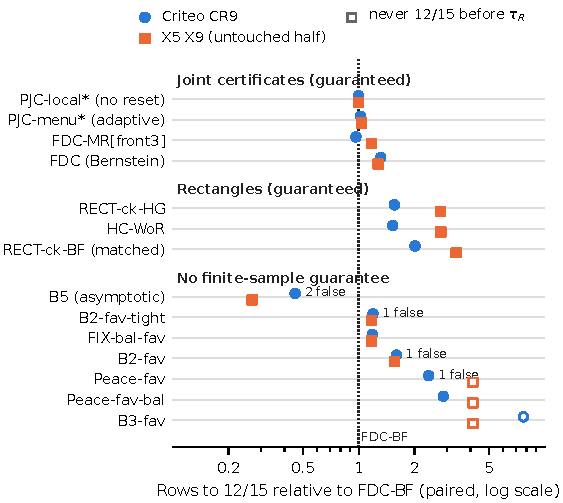
\includegraphics[width=\columnwidth]{../latex_acm/figures/fig3_speed_vs_guarantee_v8.pdf}
\caption{\textbf{Speed against guarantee, paired on both logs.} Rows to 12/15 of each method relative to FDC-BF on the same streams (1 / paired ratio; log scale; right of the dotted line = slower than FDC-BF). Criteo: Criteo-test streams (post hoc for the rows marked $^\ddagger$ in Table~\ref{tab:ckpanels}); X5: X5 test. Open markers: never 12/15 before $\tau_R$, so the value is a horizon-sensitive endpoint ratio. ``$n$ false'': streams with a false certificate; every guaranteed method has none.}
\label{fig:speed}
\Description{Dot chart with two markers per method, Criteo and X5, giving rows to 12 of 15 relative to FDC-BF on a log axis. PJC-local sits at 1.00 on both logs and PJC-menu at 1.02 to 1.03. FDC-MR is slightly left of 1 on Criteo (0.97) and right on X5 (1.17); FDC is at 1.31 and 1.27. The exact and betting rectangles are at about 1.53 to 1.56 on Criteo and 2.75 on X5; the matched Bennett rectangle is at 2.0 on Criteo and 3.3 on X5. Among rules without a guarantee, B5 is left of 1 (0.46 on Criteo with 2 false streams, 0.27 on X5); B2-fav-tight and FIX-bal-fav are at 1.17 to 1.19 and B2-fav at 1.56 to 1.59, with 1 false stream each for B2-fav-tight and B2-fav on Criteo; Peace-fav, Peace-fav-bal and B3-fav are far right on Criteo and never reach 12 of 15 on X5.}
\end{figure}

These blocks do not enter any verdict. CR12's development expectation against the exact rectangle was 0.48, so its 0.55 shows the advantage held at 4,096 policies but shrank. On the v7 streams, Neyman plans frozen from development variances made both rectangles slightly slower than their 50/50 versions (0.633 and 0.645 against 0.643 and 0.655), so the rectangles were not handicapped by the 50/50 plan. CR12's PJC-menu* difference (0.949) combines its larger union with deterministic tracking and is not attributed to either alone. One or two errors in 200 streams are compatible with a 5\% error rate, so the plug-in errors do not show a violation; plug-in rules stay descriptive because no proof covers them.


\section{Validity of the phased joint certificates}\label{app:pjc}

The phased joint certificates (PJC) are primary comparators in the X5 test and are advertised as having a proven guarantee, so this section gives the argument the main text only cites. Freezing the next phase is not enough by itself: the two PJC constructions need different arguments, a residual-pool argument for local estimation and a union over menu paths for all-data estimation.

\textbf{Setup.} Phase boundaries $b_1 < b_2 < \dots$ are data-free checkpoint indices, with $T_j$ the row count at boundary $j$ ($T_0 = 0$). The arrival sequence of segments is drawn before any outcome is read and is independent of the within-pool record orders. $\mathcal{F}_{T_j}$ is the complete observed history through the boundary checkpoint $T_j$: the arrival sequence, the queried cell identities, counts and outcomes, and the stored allocation state. Within a phase, arms are assigned by deterministic deficit tracking of the phase's target split, using the stored plan and phase counts only, never outcome sums; the replay engine assigns one arm per segment per replanning batch of $\lceil\tau_R/2000\rceil$ arrivals, at least 200 (3,495 on CR9, 200 on X5), and a new phase's plan takes effect at the first batch after its boundary. Batch edges and boundaries are data-free, so batching affects efficiency, not validity.

\begin{proposition}[PJC-local]\label{prop:pjclocal}
The split of phase $j$ may be any function of $\mathcal{F}_{T_j}$. For cell $c$ let $n_c(T_j)$ and $S_c(T_j)$ be the count and outcome sum read through $T_j$, $N'_c = N_c - n_c(T_j)$, and let $m'_c = (N_c\mu_c - S_c(T_j))/N'_c$ be the remaining-pool mean. With the phase-local estimator
\[
\hat\mu^{(j)}_c(k) = \bigl(S_c(T_j) + N'_c\,\hat m'_c(k)\bigr)/N_c,
\]
where $\hat m'_c(k)$ is the mean of the phase-$j$ reads of $c$ up to checkpoint $k$, FDC-BF's width with coefficients $a_c N'_c/N_c$ on the pools $(N'_c, m'_c)$, together with FDC-BF's exponent $\beta$ and variance level $\alpha$, gives probability of any false certificate at most $\dmain + \dvar$.
\end{proposition}
\begin{proof}
Given $\mathcal{F}_{T_j}$, the only information about pool $c$ is its first $n_c(T_j)$ records, so its unread records are in uniformly random order, independently across cells. The phase-$j$ counts $n'_c(k)$ are functions of $\mathcal{F}_{T_j}$ and the arrival sequence, so conditional on $\mathcal{F}_{T_j}$ the phase-$j$ reads of $c$ are a uniform without-replacement sample of fixed size $n'_c(k)$ from a pool of size $N'_c$ with mean $m'_c$, and Lemma A.1 applies to it. The error of the phase-local estimator is $\hat\mu^{(j)}_c - \mu_c = (N'_c/N_c)(\hat m'_c - m'_c)$, because the prefix sum $S_c(T_j)$ is known exactly; an estimator that ignored it would concentrate around $m'_c$, not $\mu_c$. For a fixed direction, $Y = \sum_c a_c(N'_c/N_c)(\hat m'_c - m'_c)$, so Lemma A.2 with coefficients $a_c N'_c/N_c$ gives $P(Y > t \mid \mathcal{F}_{T_j}) \le e^{-\beta}$ and hence unconditionally. Each checkpoint lies in exactly one phase, so the union over (problem, policy, checkpoint) has $\sum_q|\Pi_{B_q}|K$ events, as for FDC-BF. The exact hypergeometric inversion of $m'_c$ from the phase-local sample covers it with probability at least $1-2\alpha$ given $\mathcal{F}_{T_j}$; mapping to $\mu$-space by $\mu_c = (S_c(T_j) + N'_c m'_c)/N_c$ and intersecting over checkpoints keeps simultaneous coverage on $E_{\text{var}}$, whose complement has probability at most $2SAK\alpha = \dvar$. The rest is the proof of Theorem 4.1.
\end{proof}

\noindent Earlier phases enter in two ways: through the known prefix sums, and through the retained, intersected confidence boxes, which are kept in original-mean space and mapped into the current residual pool. A reset therefore discards earlier samples from the width but not all earlier information; with no boundary, PJC-local is FDC-BF with deterministic 50/50 tracking.

\begin{proposition}[PJC-menu]\label{prop:pjcmenu}
At each boundary the method chooses one of $M$ data-free designs and keeps all data, estimating $\hat\mu_c(k) = S_c(k)/n_c(k)$. Let $j(k)$ be the number of boundaries before checkpoint $k$ and $L = \sum_k M^{j(k)}$. With $L$ in place of $K$ in the exponent and the variance level, that is $\beta = \ln(L\sum_q|\Pi_{B_q}|/\dmain)$ and $\alpha = \dvar/(2SAL)$, the probability of any false certificate is at most $\dmain + \dvar$.
\end{proposition}
\begin{proof}
A menu path $p \in [M]^{j(k)}$ fixes every design up to checkpoint $k$, and under deterministic tracking the counts $n^p_c(k)$ are functions of the arrival sequence and $p$ only. For each fixed $p$, Fact 0 holds with the plan replaced by (arrival sequence, $p$), so Lemma A.2 bounds each (problem, policy, checkpoint, path) event by $e^{-\beta}$ and each (cell, checkpoint, path) box fails with probability at most $2\alpha$. The realized path is data-dependent, so its cumulative counts are not outcome-independent, and phase-by-phase application of Theorem 4.1 does not suffice. On the intersection of the events over all $L$ (path, checkpoint) pairs, however, the realized path's events hold, and the union bound charges $\sum_q|\Pi_{B_q}|L e^{-\beta} = \dmain$ and $2SAL\alpha = \dvar$.
\end{proof}

\noindent The selected PJC-menu* has $M = 2$ and one boundary after the third checkpoint, so $L = 3 + 2\cdot 17 = 37$ instead of $K = 20$: its exponent is larger by $\ln(37/20) = 0.615$ and its variance-box level smaller by the factor $20/37$. The per-segment menus of S8 choose a design per segment, so a boundary multiplies the number of paths at every later checkpoint by $M^S$; the exponent rises by $\ln(L/K)$ with $L = \sum_k M^{S j(k)}$, which for the selected three-option member, whose boundary follows the ninth checkpoint, is $\ln[(9 + 11\cdot 3^9)/20] = 9.29$ (slightly less than $S\ln M = 9.89$). All post-hoc members of S8 are instances of one of these two propositions.

\section{Post-hoc check with adaptive joint variants}\label{app:adaptive}

\begin{table*}[t]
\caption{\textbf{Adaptive joint variants against FDC-BF} (post hoc, descriptive; run after the X5 test). All members are in FDC-BF's guarantee class (Propositions~\ref{prop:pjclocal} and~\ref{prop:pjcmenu}). Families: \emph{reset} = RAGE-style phases with residual-pool estimation and per-segment Neyman or direction-optimal splits; \emph{menu} = all data, one global control share from \{0.3, \dots, 0.7\} per boundary; \emph{segmenu} = all data, a share per segment from a menu. Boundaries: 1--3 (2--4 phases); 64 members per log. Picks tuned on development seeds 900--949 (smallest geometric-mean $\Npen$). Ratio = paired geometric mean of FDC-BF / variant [95\% CI] ($<1$: FDC-BF reads fewer rows). Switched = share of streams whose design left 50/50 before the twelfth certification. Every member on both logs had 0/200 false streams and a ratio below 1 with CI upper bound below 1; on a near-tie toy, eight representative members had 0/200 false streams each.}
\label{tab:adaptive}
\small
\begin{tabular}{@{}llrrr@{}}
\toprule
Log & Family: development-tuned pick & FDC-BF / variant [95\% CI] & Variant $N/\tau_R$ & Switched \\
\midrule
X5 X9 (seeds 35000--35199, $\eps = 0.02$) & reset, 1 boundary, Neyman & 0.924 [0.910, 0.937] & 0.263 & 100\% \\
& menu, 1 boundary, projected variance & 0.943 [0.930, 0.955] & 0.258 & 0\% \\
& segmenu \{0.3, 0.5, 0.7\}, 1 boundary, Neyman & 0.686 [0.675, 0.697] & 0.354 & 0\% \\
& best of 64 chosen on evaluation streams (menu) & 0.943 [0.930, 0.955] & 0.258 & 0\% \\
\midrule
Criteo CR9 (seeds 33000--33199, $\eps = 0.001$) & reset, 1 boundary, Neyman & 0.951 [0.930, 0.972] & 0.137 & 100\% \\
& menu, 1 boundary, projected variance & 0.933 [0.917, 0.949] & 0.139 & 0\% \\
& segmenu \{0.3, 0.5, 0.7\}, 1 boundary, Neyman & 0.670 [0.654, 0.686] & 0.194 & 15\% \\
& best of 64 chosen on evaluation streams (reset) & 0.951 [0.930, 0.972] & 0.137 & 100\% \\
\bottomrule
\end{tabular}
\end{table*}

The registered PJC members never changed their design on X5, so the registered non-inferiority test could not show whether adaptation helps; Table~\ref{tab:adaptive} adds members that do. Members, grid and tuning rule were fixed before any evaluation row of this block was computed, evaluation access went through a logged post-hoc path, and FDC-BF's sealed rows were reproduced on all 200 streams of each log. The block is nevertheless post hoc: its existence, members and grid were chosen knowing the confirmatory outcome, and the ``best of 64'' rows are selected on evaluation data and therefore optimistic for the variants. On X5 the reset family moved off 50/50 on 52\% of member-stream pairs on average, the global menu on none and the per-segment menu on 2\%; on Criteo the shares were 97\%, 0.3\% and 68\%. Thirty-seven Criteo members and eight X5 members switched on at least half the streams, and the best of them read 5\% (Criteo) and 8\% (X5) more rows than FDC-BF.

The pattern has a structural explanation. Within each segment the two arms have nearly equal Bernoulli variances, so the variance-optimal within-segment split is close to 50/50; a free global menu therefore keeps 0.5 and pays only its larger union. Members that do move the design pay for it in another way: the reset discards earlier-phase samples, and the per-segment menu multiplies its path count by $M^S$ at each boundary (9.29 added to the exponent for the selected member), which outweighs any reallocation gain. This holds for logs whose arrivals are fixed and whose arm variances are near-equal; S11 tests very unequal arm variances on semi-synthetic pools, where adaptive designs do beat the 50/50 plan; at equal pilot information a frozen pilot-Neyman plan beats the tested adaptive designs, also with the pilot charged to both; against adaptive designs without a pilot, charging it to the frozen plan alone reverses the comparison on small tables unless the pilot is shared. A certifier that chooses which segment arrives remains untested.

\section{What remains untested}\label{app:sens}

The r4 blocks measure what the r3 version listed as untested: $\delta$, $\dvar$, $K$, the $\lambda$ grid and the replanning batch size (S10) and strongly unequal arm variances (S11). Four gaps remain. (i) \emph{Endpoint.} Only the 12-of-15 endpoint is primary; the full-frontier $N_{100}$ ratios (Table 1) are the only check on a different endpoint, and $\eps$ was varied only on X5, Lenta and Hillstrom. (ii) \emph{Arrival control.} In every block the log fixes which segment arrives next; a certifier that chooses arrivals could gain from adaptivity in a way none of our blocks measures. (iii) \emph{Scale.} Locks v7--v9 enumerate classes of up to 4,096 policies; lock v10 (S17) certifies implicit classes of up to $2^{64}$ policies, but only with cardinality budgets, two arms and tolerances chosen by a development rule that places the rival at its penultimate checkpoint. At 16 to 64 segments, heterogeneous knapsack costs were tested only descriptively, on development halves with simulated (X5) or proxy (Lenta) costs (block G2, S19). The one confirmatory knapsack test is lock v11 (S21), with nine segments, 512 policies, one tolerance and traffic-share rather than monetary costs, so no confirmatory test covers knapsack costs on large classes. (iv) \emph{Preregistration of the r4 blocks.} S10--S13 are descriptive development-half results. Lock v9 confirmed only the dense-monitoring comparison: block A (Criteo, seeds 37000--37199) and block B (X5, 37200--37399) both returned \emph{positive result achieved} (TU-FDC / HC-WoR* 0.708, UB95 0.723, and 0.374, UB95 0.379; TU-FDC / RECT-ck-BF-TU 0.530, UB95 0.542, and 0.304, UB95 0.308; non-inferiority UB95 0.992 against PJC-local* and 1.009 against TU-PJC; Table~\ref{tab:v9}), and block C (Hillstrom, 37400--37599) is a descriptive reuse with the wording ``faster (descriptive)'' (S13). The sensitivity, regime and ablation blocks have no confirmatory counterpart. These gaps bound the scope of the robustness claims in Section 6.7 of the paper.

\section{Sensitivity to the registered knobs}\label{app:sensE}

Table~\ref{tab:sens} varies one registered knob at a time on the development halves, with rival configurations frozen at their lock-v8 values; the knob values were fixed before any row of the block was computed, and no evaluation row was read. Against the rectangles, FDC-BF stays between 0.27 and 0.36 on X5 and between 0.50 and 0.69 on Criteo, with every CI upper limit below 1; against PJC-local* it stays between 0.976 and 1.016, with the largest upper 95\% CI limit 1.037 (Criteo, total $\delta = 0.01$), inside the registered 1.05 margin. The $\lambda$ grid density changes no $N_{80}$ row of FDC-BF or RECT-ck-BF, $\dvar$ moves FDC-BF by at most 2\%, and halving or doubling the replanning batch changes FDC-BF/PJC by at most 0.02. Proposition 4.3 predicts that a smaller $\delta$ favours the joint width because $\beta_J/\beta_C$ falls from 1.47 to 1.40 at $\dmain = 0.009$; this held on Criteo (FDC-BF/RECT-ck-HG* 0.613 against 0.649) and not on X5, where both $\delta$ changes moved the ratio slightly toward the rectangle. No method made a false certificate in 5,500 method-setting-stream runs. The ordering of C2 and the non-inferiority to PJC-local* therefore persisted over the tested settings; one-at-a-time variation on a finite development grid does not establish robustness outside it.

% copied by writing/scripts/gen_r4_supp_tables.py from exp/results/full/v8_posthoc_E/table.tex
% v8-posthoc-E (post hoc, descriptive, dev halves only; generated by exp/code/run_v8_posthoc_E.py)
\begin{table*}[t]
\caption{\textbf{Sensitivity (post hoc, descriptive, development halves, 50 streams per cell, seeds 950--999).} Paired geometric-mean ratio FDC-BF/rival of $\Npen$ with 95\% bootstrap CI ($<1$: FDC-BF reads fewer rows); X5 at $\eps=0.02$, CR9 at $\eps=0.001$. Baseline: $K=20$, $\delta=0.05$ split 0.045/0.005, 161-point $\lambda$ grid, registered replanning batch. Rivals without the varied knob keep their baseline rows; rival configurations are the frozen lock-v8 ones. FS: false streams of FDC-BF / of all methods run at that setting.}
\label{tab:sens}
\scriptsize
\setlength{\tabcolsep}{3pt}
\begin{tabular}{@{}llllllll@{}}
\toprule
Setting & RECT-ck-HG* & HC-WoR* & RECT-ck-BF & PJC-local* & PJC-menu* & PJC reset & FS \\
\midrule
\multicolumn{8}{@{}l}{\emph{X5 RetailHero (development half), $\tau_R=99{,}646$}} \\
baseline & 0.34 [0.32, 0.35] & 0.33 [0.32, 0.34] & 0.31 [0.29, 0.32] & 0.99 [0.97, 1.01] & 0.93 [0.90, 0.95] & 0.91 [0.88, 0.94] & 0/0 \\
$\delta_{\mathrm{var}}=0.0025$ & -- & -- & 0.30 [0.29, 0.32] & 0.99 [0.97, 1.02] & 0.93 [0.91, 0.96] & 0.91 [0.88, 0.94] & 0/0 \\
$\delta_{\mathrm{var}}=0.01$ & -- & -- & 0.31 [0.30, 0.32] & 1.00 [0.99, 1.02] & 0.94 [0.92, 0.97] & 0.92 [0.89, 0.94] & 0/0 \\
$\delta=0.01$ & 0.35 [0.34, 0.36] & 0.35 [0.34, 0.35] & 0.35 [0.34, 0.35] & 1.00 [0.98, 1.03] & 0.97 [0.95, 0.99] & 0.95 [0.92, 0.98] & 0/0 \\
$\delta=0.10$ & 0.34 [0.33, 0.36] & 0.34 [0.33, 0.35] & 0.29 [0.28, 0.31] & 1.00 [0.98, 1.02] & 0.96 [0.94, 0.99] & 0.92 [0.89, 0.95] & 0/0 \\
$K=10$ & 0.34 [0.32, 0.37] & 0.29 [0.27, 0.30] & 0.27 [0.26, 0.27] & 0.99 [0.97, 1.00] & 0.98 [0.96, 1.00] & 0.93 [0.89, 0.97] & 0/0 \\
$K=40$ & 0.35 [0.34, 0.36] & 0.36 [0.35, 0.37] & 0.31 [0.30, 0.32] & 1.00 [0.99, 1.02] & 0.97 [0.95, 0.98] & 0.94 [0.92, 0.96] & 0/0 \\
$\lambda$ grid 81 & -- & -- & 0.31 [0.29, 0.32] & -- & -- & -- & 0/0 \\
$\lambda$ grid 321 & -- & -- & 0.31 [0.29, 0.32] & -- & -- & -- & 0/0 \\
replan $\times 0.5$ & -- & -- & -- & 0.98 [0.95, 1.00] & 0.93 [0.91, 0.96] & 0.91 [0.88, 0.94] & 0/0 \\
replan $\times 2$ & -- & -- & -- & 0.98 [0.96, 1.00] & 0.95 [0.92, 0.97] & 0.91 [0.88, 0.94] & 0/0 \\
\midrule
\multicolumn{8}{@{}l}{\emph{Criteo CR9 (development half), $\tau_R=6{,}989{,}793$}} \\
baseline & 0.65 [0.62, 0.68] & 0.66 [0.63, 0.70] & 0.52 [0.49, 0.56] & 1.00 [0.98, 1.02] & 0.97 [0.95, 0.99] & 0.92 [0.88, 0.95] & 0/0 \\
$\delta_{\mathrm{var}}=0.0025$ & -- & -- & 0.52 [0.49, 0.56] & 1.00 [0.98, 1.02] & 0.97 [0.95, 0.99] & 0.92 [0.88, 0.95] & 0/0 \\
$\delta_{\mathrm{var}}=0.01$ & -- & -- & 0.52 [0.49, 0.56] & 0.99 [0.97, 1.00] & 0.97 [0.94, 0.99] & 0.92 [0.88, 0.95] & 0/0 \\
$\delta=0.01$ & 0.61 [0.58, 0.65] & 0.62 [0.59, 0.64] & 0.50 [0.47, 0.52] & 1.01 [0.99, 1.04] & 0.98 [0.96, 0.99] & 0.93 [0.91, 0.96] & 0/0 \\
$\delta=0.10$ & 0.65 [0.61, 0.68] & 0.65 [0.61, 0.69] & 0.50 [0.47, 0.53] & 1.01 [0.98, 1.03] & 0.94 [0.92, 0.97] & 0.89 [0.85, 0.93] & 0/0 \\
$K=10$ & 0.62 [0.58, 0.67] & 0.61 [0.57, 0.67] & 0.52 [0.47, 0.56] & 0.98 [0.94, 1.02] & 0.93 [0.88, 0.97] & 0.90 [0.84, 0.96] & 0/0 \\
$K=40$ & 0.63 [0.60, 0.67] & 0.69 [0.65, 0.72] & 0.50 [0.47, 0.53] & 1.00 [0.99, 1.01] & 0.97 [0.96, 0.99] & 0.92 [0.88, 0.96] & 0/0 \\
$\lambda$ grid 81 & -- & -- & 0.52 [0.49, 0.56] & -- & -- & -- & 0/0 \\
$\lambda$ grid 321 & -- & -- & 0.52 [0.49, 0.56] & -- & -- & -- & 0/0 \\
replan $\times 0.5$ & -- & -- & -- & 1.01 [1.00, 1.03] & 0.97 [0.95, 0.99] & 0.92 [0.88, 0.96] & 0/0 \\
replan $\times 2$ & -- & -- & -- & 1.02 [1.00, 1.04] & 0.96 [0.93, 0.98] & 0.92 [0.89, 0.96] & 0/0 \\
\bottomrule
\end{tabular}
\end{table*}


\section{Adaptive regime: strongly unequal arm variances}\label{app:regime}

The real logs have near-equal arm variances, so this block asks whether adaptation helps when the variance-optimal split is far from 50/50. It keeps the development halves' segment and arm labels, pool sizes, weights and frozen arrival schedules and replaces every outcome by a synthetic Bernoulli pool with exactly round(rate $\times N_c$) ones: \emph{asym} draws control rates from 0.02--0.05 and treatment rates from 0.40--0.50 in every segment (Neyman control share about 0.25--0.30), and \emph{mixed} cycles three segment types with Neyman control shares about 0.27, 0.70 and 0.50. Rates, regimes, the $\eps$ rule, the method list and the adaptive grid were fixed before any row; $\eps$ was calibrated with frozen 50/50 FDC-BF only (seeds 900--919), adaptive picks were tuned on seeds 900--949, and 250 reporting streams (950--999 and 36000--36199) were used for nothing else. The pilot-Neyman plan of block F uses an independent pilot of 1,000 Bernoulli draws per cell from the same rates, the analogue of a development half; its 18,000 pilot reads per instance are not counted in $N_{80}$ (block F2 below charges them).

Table~\ref{tab:posthocF} shows that adaptation can beat frozen 50/50 FDC-BF in one regime: on Criteo-asym the registered PJC-menu* and the tuned reset and global-menu picks read 8.0--11.3\% fewer rows than FDC-BF (FDC-BF/method 1.087--1.127, a read reduction of $1 - 1/r$). In the same regime frozen pilot-Neyman FDC-BF reads 15.2\% fewer rows than 50/50 (ratio 1.180) and faster than the best adaptive pick (0.955 [0.940, 0.970]), and across the four regimes pilot-Neyman/best adaptive lies between 0.938 and 0.973 with every CI below 1. On X5-asym the gains shrink to a few percent, consistent with X5's 50/50 pools (a conjecture this block does not isolate), and in the mixed regimes no adaptive member beats frozen 50/50 while the per-segment menu pays $M^S$ paths per boundary and reads 25.7\% and 53.9\% more rows than FDC-BF (ratios 0.795 and 0.650, extra reads $1/r - 1$). Neyman shares are not optimal for Bennett widths, because cells read less pay the range term $b\beta/3$, which caps every Neyman-type gain. No method in any regime had a false stream. Because the pilot in block F is free and the adaptive picks start without it, block F alone does not separate allocation from information.

% adapted (table -> table*) by writing/scripts/gen_r4_supp_tables.py from exp/results/full/v8_posthoc_F/table.tex
% v8-posthoc-F (POST-HOC, DESCRIPTIVE, SEMI-SYNTHETIC); generated by exp/code/run_v8_posthoc_F.py
\begin{table*}[t]
\centering\small
\setlength{\tabcolsep}{3pt}
\caption{Semi-synthetic, post-hoc, descriptive: arm-variance asymmetry. Paired geometric-mean ratio FDC-BF (frozen 50/50) / method of $N_{80}$ with 95\% bootstrap CI over 250 streams ($<1$: FDC-BF faster). Structure from the X5 and Criteo development halves; outcomes synthetic (asym: control 0.02--0.05 vs treatment 0.40--0.50 in every segment; mixed: three segment types with Neyman control shares $\approx$0.27/0.70/0.50). Adaptive PJC-A picks tuned on separate seeds. No method had a false certification stream.}
\label{tab:posthocF}
\begin{tabular}{lcccc}
\toprule
Method & X5-asym & X5-mixed & Criteo-asym & Criteo-mixed \\
 & $\varepsilon=0.015$ & $\varepsilon=0.02$ & $\varepsilon=0.001$ & $\varepsilon=0.00075$ \\
\midrule
FDC-BF, frozen pilot-Neyman & 1.04 [1.02, 1.05] & 0.99 [0.98, 1.00] & 1.18 [1.15, 1.21] & 1.03 [1.01, 1.05] \\
FDC-BF, frozen oracle-Neyman & 1.04 [1.03, 1.06] & 0.99 [0.98, 1.01] & 1.18 [1.15, 1.20] & 1.04 [1.02, 1.05] \\
RECT-ck-HG & 0.43 [0.42, 0.44] & 0.38 [0.37, 0.39] & 0.67 [0.65, 0.69] & 0.78 [0.76, 0.79] \\
RECT-ck-HG, pilot-Neyman & 0.46 [0.46, 0.47] & 0.42 [0.41, 0.42] & 0.54 [0.53, 0.56] & 0.78 [0.77, 0.80] \\
RECT-ck-BF & 0.36 [0.36, 0.37] & 0.34 [0.33, 0.34] & 0.56 [0.54, 0.57] & 0.69 [0.67, 0.70] \\
RECT-ck-BF, pilot-Neyman & 0.44 [0.44, 0.45] & 0.34 [0.34, 0.35] & 0.48 [0.47, 0.49] & 0.68 [0.66, 0.69] \\
HC-WoR & 0.42 [0.41, 0.43] & 0.39 [0.38, 0.39] & 0.67 [0.65, 0.68] & 0.77 [0.75, 0.78] \\
HC-WoR, pilot-Neyman & 0.45 [0.44, 0.45] & 0.41 [0.41, 0.42] & 0.53 [0.52, 0.55] & 0.78 [0.77, 0.80] \\
PJC-local$^*$ & 0.99 [0.99, 1.00] & 1.00 [0.99, 1.01] & 1.00 [0.99, 1.01] & 1.00 [0.99, 1.00] \\
PJC-menu$^*$ & 1.05 [1.04, 1.07] & 0.96 [0.95, 0.97] & 1.09 [1.07, 1.11] & 0.94 [0.92, 0.96] \\
\midrule
PJC-A reset (tuned) & 0.96 [0.95, 0.98] (1.00) & 0.90 [0.89, 0.92] (1.00) & 1.13 [1.10, 1.15] (1.00) & 1.00 [0.99, 1.02] (1.00) \\
PJC-A global menu (tuned) & 1.01 [0.99, 1.02] (1.00) & 0.93 [0.92, 0.94] (0.00) & 1.10 [1.08, 1.12] (1.00) & 0.92 [0.90, 0.94] (0.86) \\
PJC-A per-segment menu (tuned) & 0.72 [0.71, 0.73] (1.00) & 0.65 [0.64, 0.66] (1.00) & 0.80 [0.79, 0.82] (1.00) & 0.80 [0.78, 0.81] (1.00) \\
\bottomrule
\end{tabular}
\\[2pt]{\footnotesize Parentheses after adaptive rows: fraction of streams whose design moved off 50/50.}
\end{table*}


\textbf{Block F2: equal information and charged pilot reads.} Block F2 (post hoc, semi-synthetic, descriptive; \texttt{exp/results/full/v8\_posthoc\_F2}) reuses block F's environments, tolerances, reporting seeds and adaptive picks. Each stream draws one independent pilot of $n \in \{250, 1000\}$ with-replacement draws per cell from the exact pool means, nested across $n$ and shared by every method on that stream; an instance costs $SAn$ = 4,500 or 18,000 reads. A without-replacement prefix of the replay was not used, because a plan computed from replay reads is not independent of the replay permutation. With a pilot, the adaptive picks start from the pilot's per-segment Neyman plan (\emph{init}) and also pool the pilot counts into every variance plug-in of their design rule (\emph{init+warm}); their certificates use replay data only and their ledgers are unchanged. Charged rows add $SAn/J$ to $N_{80}$, where $J \in \{1, 4, 16, \infty\}$ is the number of certification runs sharing one pilot. These choices were fixed before any F2 row, and block F's pilot-free rows were reproduced on 30 of 30 checks per regime.

Table~\ref{tab:posthocF2h2h} gives the head-to-head ratios. At equal information, frozen pilot-Neyman FDC-BF reads fewer rows than every tested reset and menu design in all four regimes and at both pilot sizes: across \emph{init} and \emph{init+warm} and every $J$, including $J = 1$ (pilot charged in full to both sides), the 128 ratios lie between 0.90 and 0.98, each with a 95\% CI below 1 (largest upper limit 0.995). The pilot hardly helps the adaptive designs (Criteo-asym reset 1.127 without and 1.125 with the 1,000-draw pilot, as FDC-BF / method), because the reset member discards pre-boundary data and the menu member pays its path-union ledger even when it rarely leaves the pilot plan. A different comparison charges the pilot to the frozen plan alone, against the adaptive picks learning without one; its result depends on the table size. On Criteo-structured tables ($\tau_R$ = 7.0M) the pilot is 0.06--0.26\% of $\tau_R$, and the point estimates still favour frozen pilot-Neyman FDC-BF, which needs 0.89--0.99 times the rows of the no-pilot picks; one of the eight intervals, 0.990 [0.975, 1.005] (CR9-mixed, $n$ = 1,000, reset), includes 1. On X5-structured tables ($\tau_R \approx 100$k) the pilot is 4.5\% or 18\% of $\tau_R$ and the comparison reverses (1.08--1.67). The point-estimate break-even number of runs sharing one pilot is $J$ = 2.1--25.5, that is 3 to 26 whole runs; it is not a simultaneous inferential guarantee. Table~\ref{tab:posthocF2} gives the per-method rows. No method had a false stream (0/250 per method and regime). No phase-wise time-uniform wrapper was built for the adaptive designs, so all F2 comparisons are at checkpoint strength. An informed frozen plan therefore beats these reset and menu implementations at equal information in the four tested regimes, even with the pilot charged to both sides. Against pilot-free adaptation on small tables it pays off only when its pilot already exists or is amortised over several runs, and since the adaptive picks were not retuned with a pilot, F2 says nothing about the best adaptive allocation.

% generated by writing/scripts/gen_r5_supp_tables.py from exp/results/full/v8_posthoc_F2/summary.json
\begin{table*}[t]
\caption{\textbf{Block F2: frozen pilot-Neyman FDC-BF against the adaptive picks} (semi-synthetic, post hoc, descriptive; 250 streams per regime). Ratio = paired geometric mean of $N_{80}$, frozen pilot-Neyman FDC-BF / adaptive design, with 95\% bootstrap CI ($<1$: the frozen plan reads fewer rows). \emph{Equal information}: the adaptive design receives the same per-stream pilot (phase-0 pilot-Neyman plan plus pooled variance warm start) and both sides pay the same pilot. \emph{Charged pilot}: the frozen plan pays its pilot in full ($J = 1$) and the adaptive pick learns without a pilot; break-even $J$ = number of certification runs that must share one pilot before the frozen plan is faster. No method had a false stream.}
\label{tab:posthocF2h2h}
\small
\setlength{\tabcolsep}{3pt}
\begin{tabular}{@{}lrllllll@{}}
\toprule
& & \multicolumn{2}{c}{Equal information ($J = 1$)} & \multicolumn{4}{c}{Charged pilot vs no-pilot adaptive pick ($J = 1$)} \\
Regime & Pilot $n$ & vs reset & vs menu & vs reset & break-even $J$ & vs menu & break-even $J$ \\
\midrule
X5-asym & 250 & 0.941 {\scriptsize[0.930, 0.951]} & 0.928 {\scriptsize[0.917, 0.938]} & 1.078 {\scriptsize[1.063, 1.092]} & 2.10 & 1.129 {\scriptsize[1.116, 1.143]} & 5.98 \\
X5-asym & 1,000 & 0.958 {\scriptsize[0.950, 0.966]} & 0.951 {\scriptsize[0.944, 0.959]} & 1.523 {\scriptsize[1.504, 1.542]} & 8.58 & 1.596 {\scriptsize[1.579, 1.613]} & 25.50 \\
X5-mixed & 250 & 0.925 {\scriptsize[0.914, 0.937]} & 0.949 {\scriptsize[0.940, 0.959]} & 1.095 {\scriptsize[1.080, 1.109]} & 2.09 & 1.125 {\scriptsize[1.110, 1.140]} & 3.03 \\
X5-mixed & 1,000 & 0.943 {\scriptsize[0.935, 0.951]} & 0.954 {\scriptsize[0.947, 0.961]} & 1.629 {\scriptsize[1.609, 1.650]} & 7.71 & 1.674 {\scriptsize[1.653, 1.696]} & 10.78 \\
Criteo-asym & 250 & 0.971 {\scriptsize[0.954, 0.989]} & 0.943 {\scriptsize[0.928, 0.955]} & 0.975 {\scriptsize[0.958, 0.993]} & 1.00 & 0.953 {\scriptsize[0.937, 0.968]} & 1.00 \\
Criteo-asym & 1,000 & 0.962 {\scriptsize[0.946, 0.978]} & 0.938 {\scriptsize[0.925, 0.951]} & 0.975 {\scriptsize[0.959, 0.990]} & 1.00 & 0.953 {\scriptsize[0.938, 0.967]} & 1.00 \\
Criteo-mixed & 250 & 0.971 {\scriptsize[0.956, 0.986]} & 0.959 {\scriptsize[0.947, 0.972]} & 0.973 {\scriptsize[0.958, 0.987]} & 1.00 & 0.894 {\scriptsize[0.878, 0.912]} & 1.00 \\
Criteo-mixed & 1,000 & 0.977 {\scriptsize[0.961, 0.992]} & 0.961 {\scriptsize[0.949, 0.972]} & 0.990 {\scriptsize[0.975, 1.005]} & 1.00 & 0.910 {\scriptsize[0.893, 0.929]} & 1.00 \\
\bottomrule
\end{tabular}
\end{table*}

% adapted (table -> table*) by writing/scripts/gen_r5_supp_tables.py from exp/results/full/v8_posthoc_F2/table.tex
% v8-posthoc-F2 (POST-HOC, DESCRIPTIVE, SEMI-SYNTHETIC); generated by exp/code/run_v8_posthoc_F2.py
\begin{table*}[t]
\centering\small
\setlength{\tabcolsep}{2.5pt}
\caption{Semi-synthetic, post-hoc, descriptive: pilot versus adaptive allocation with the pilot charged. Paired geometric-mean ratio FDC-BF (frozen 50/50, no pilot) / method of $N_{80}$ with 95\% bootstrap CI over 250 streams ($>1$: method faster). Pilot reads ($18n$ per instance, $n$ per cell, independent draws from the same pools) are added to the method's $N_{80}$ in full ($J{=}1$) or amortised over $J{=}16$ instances. Adaptive PJC-A picks are block F's (tuned without a pilot); with a pilot they start from the pilot Neyman plan and warm-start their variance plug-ins. No method had a false certification stream.}
\label{tab:posthocF2}
\begin{tabular}{llcccc}
\toprule
Method & $J$ & X5-asym & X5-mixed & Criteo-asym & Criteo-mixed \\
\midrule
PJC-A reset, no pilot & -- & 0.962 {\scriptsize[0.947, 0.977]} & 0.904 {\scriptsize[0.890, 0.919]} & 1.127 {\scriptsize[1.102, 1.153]} & 1.003 {\scriptsize[0.986, 1.021]} \\
PJC-A menu, no pilot & -- & 1.008 {\scriptsize[0.992, 1.025]} & 0.929 {\scriptsize[0.917, 0.942]} & 1.102 {\scriptsize[1.079, 1.125]} & 0.922 {\scriptsize[0.905, 0.940]} \\
\midrule
FDC-BF pilot-Neyman, $n{=}250$ & 1 & 0.893 {\scriptsize[0.879, 0.907]} & 0.826 {\scriptsize[0.816, 0.836]} & 1.156 {\scriptsize[1.133, 1.180]} & 1.031 {\scriptsize[1.014, 1.048]} \\
FDC-BF pilot-Neyman, $n{=}250$ & 16 & 1.025 {\scriptsize[1.008, 1.042]} & 0.978 {\scriptsize[0.965, 0.991]} & 1.159 {\scriptsize[1.136, 1.183]} & 1.034 {\scriptsize[1.017, 1.051]} \\
PJC-A reset + pilot, $n{=}250$ & 1 & 0.840 {\scriptsize[0.827, 0.853]} & 0.765 {\scriptsize[0.753, 0.776]} & 1.123 {\scriptsize[1.097, 1.148]} & 1.001 {\scriptsize[0.983, 1.020]} \\
PJC-A reset + pilot, $n{=}250$ & 16 & 0.956 {\scriptsize[0.940, 0.971]} & 0.893 {\scriptsize[0.879, 0.907]} & 1.126 {\scriptsize[1.100, 1.152]} & 1.004 {\scriptsize[0.985, 1.023]} \\
PJC-A menu + pilot, $n{=}250$ & 1 & 0.828 {\scriptsize[0.815, 0.842]} & 0.785 {\scriptsize[0.774, 0.795]} & 1.089 {\scriptsize[1.067, 1.112]} & 0.989 {\scriptsize[0.972, 1.006]} \\
PJC-A menu + pilot, $n{=}250$ & 16 & 0.941 {\scriptsize[0.925, 0.957]} & 0.920 {\scriptsize[0.907, 0.934]} & 1.092 {\scriptsize[1.070, 1.115]} & 0.992 {\scriptsize[0.974, 1.008]} \\
\midrule
FDC-BF pilot-Neyman, $n{=}1000$ & 1 & 0.632 {\scriptsize[0.623, 0.641]} & 0.555 {\scriptsize[0.549, 0.562]} & 1.156 {\scriptsize[1.131, 1.181]} & 1.013 {\scriptsize[0.996, 1.030]} \\
FDC-BF pilot-Neyman, $n{=}1000$ & 16 & 0.994 {\scriptsize[0.978, 1.010]} & 0.951 {\scriptsize[0.938, 0.963]} & 1.169 {\scriptsize[1.144, 1.195]} & 1.023 {\scriptsize[1.007, 1.041]} \\
PJC-A reset + pilot, $n{=}1000$ & 1 & 0.605 {\scriptsize[0.597, 0.614]} & 0.524 {\scriptsize[0.516, 0.531]} & 1.111 {\scriptsize[1.086, 1.137]} & 0.989 {\scriptsize[0.970, 1.008]} \\
PJC-A reset + pilot, $n{=}1000$ & 16 & 0.930 {\scriptsize[0.916, 0.944]} & 0.863 {\scriptsize[0.848, 0.877]} & 1.124 {\scriptsize[1.098, 1.150]} & 0.999 {\scriptsize[0.980, 1.018]} \\
PJC-A menu + pilot, $n{=}1000$ & 1 & 0.601 {\scriptsize[0.593, 0.609]} & 0.530 {\scriptsize[0.523, 0.537]} & 1.084 {\scriptsize[1.061, 1.108]} & 0.973 {\scriptsize[0.956, 0.989]} \\
PJC-A menu + pilot, $n{=}1000$ & 16 & 0.920 {\scriptsize[0.907, 0.934]} & 0.879 {\scriptsize[0.866, 0.892]} & 1.096 {\scriptsize[1.073, 1.120]} & 0.983 {\scriptsize[0.966, 0.999]} \\
\bottomrule
\end{tabular}
\end{table*}


\section{Ablations and the time-uniform block}\label{app:ablation}

Table~\ref{tab:ablation} reports the two upgrade candidates and the dense-monitoring block, all on development halves. \emph{FDC-HG} keeps FDC-BF's plan, union, ledger, $\lambda$ grid and variance boxes and replaces each cell's Bennett bound by the upper envelope, over the integer pool counts in the variance box, of the exact hypergeometric log-MGF; it is valid by the same Chernoff argument and never wider than FDC-BF, but at the checkpoints that decide $N_{80}$ the cells hold $10^4$--$10^5$ reads, where Bennett and the exact log-MGF differ only in third-order terms, so it read 2--6\% fewer rows (its pre-stated go criterion, UB95 $<$ 0.90 on one log, failed; certificate time up to 7.1\,s per checkpoint). \emph{FDC-LOC} replaces $\beta_J$ at each checkpoint by the smallest $\beta$ whose gap-weighted union $\sum_{q,\pi}\exp(-\beta(1 + (\Delta^{\text{lo}}_{q,\pi} - \eps)_+/\bar W_{q,\pi}(\beta)))$ is at most $\dmain/K$, with gap lower bounds and width upper bounds computed on the variance boxes already paid for; it is valid because a deterministic comparator built from the true gaps is dominated on $E_{\text{var}}$, and it never exceeds $\beta_J$. It gained 7.5\% on Criteo and nothing on X5: at certification, $\hat\beta/\beta_J$ was 0.944 on Criteo and 1.000 on X5. The true-gap census explains why: on the X5 development half 3,076 of 3,347 (problem, policy) pairs are $\eps$-optimal and all lie within $2\eps$, and on Criteo 437 of 3,386 are $\eps$-optimal and 1,531 lie within $3\eps$, so few pairs can be excluded before certification; an invalid oracle that knows the gaps reaches about 0.81. The dense block evaluates every method at 77 times; FDC-BF with stale widths keeps its advantage over HC-WoR (0.708 and 0.356), dense monitoring helps HC-WoR more (about 10\%) than FDC-BF (2--5\%), and refreshing FDC-BF's widths at all 77 times buys nothing because $\ln(77/20)$ in the exponent cancels the fresher widths. The ablations thus place the saving in the joint geometry rather than in the cell inequality or the ledger.

\textbf{Lock-v9 time-uniform test.} Table~\ref{tab:v9} reports every registered row of the confirmatory dense-monitoring blocks on fresh streams (Criteo seeds 37000--37199, X5 seeds 37200--37399), with the thresholds and decision rules of \texttt{plan/prereg\_lock\_v9\_addendum.md}. Both blocks returned \emph{positive result achieved}: TU-FDC / HC-WoR* 0.708 (UB95 0.723) and TU-FDC / RECT-ck-BF-TU 0.530 (UB95 0.542) on Criteo, under the 0.85 threshold, and 0.374 (UB95 0.379) and 0.304 (UB95 0.308) on X5, under 0.50; on X5 TU-FDC is non-inferior to PJC-local* with its 77-time ledger (0.985, UB95 0.992) and to TU-PJC (1.004, UB95 1.009), within the 1.05 margin, which supports ``matches PJC'' and not ``faster than PJC''. No rigorous method had a false stream, and every replica check passed, including the cross-grid check R2c of each method's own schedule digest and cell counts. The development pattern holds on the evaluation streams: dense monitoring cut HC-WoR*'s rows more than TU-FDC's ($\Npen/\tau_R$ 0.197 to 0.176 against 0.130 to 0.125 on Criteo), so on the same lock-v9 streams denser monitoring moved FDC-BF's ratio against HC-WoR* from 0.658 at the 20 checkpoints to 0.708 at 77 times on Criteo and from 0.364 to 0.374 on X5. This is a within-v9 monitoring comparison, not a price of guarantee strength: FDC-BF is already time-uniform on its frozen plan at $K = 20$; refreshing FDC-BF's widths at all 77 times (FDC-BF[K77]) changed nothing material, and the no-go candidates FDC-HG and FDC-LOC, now descriptive, read 2\% and 6\% fewer rows than FDC-BF on Criteo and 2\% and 0\% on X5. The confirmation is conditional on the two reused finite tables, covers only the two registered rectangle constructions, rests on a post-hoc time-uniform reading of an unchanged procedure, and leaves HC-WoR's validity under adaptive sampling, which TU-FDC lacks, unused.

% generated by writing/scripts/gen_r4_supp_tables.py -- do not edit by hand
\begin{table*}[t]
\caption{\textbf{Lock v9, blocks A (Criteo CR9, seeds 37000--37199, $\eps = 0.001$) and B (X5 X9 evaluation half, seeds 37200--37399, $\eps = 0.02$)}: every registered row, 200 paired streams per block. Upper panel: every method monitored at the same 77 times; ratio = TU-FDC / method, paired geometric mean of $\Npen$ with 95\% CI and one-sided UB95 in parentheses; F/T/S = \% of streams on which TU-FDC stops earlier / at the same time / later. Lower panel: the 20-checkpoint grid, ratio = FDC-BF / method. Verdicts: A positive result achieved (governing UB95 0.723, threshold 0.85); B positive result achieved (governing UB95 0.379, threshold 0.50; non-inferiority UB95 1.009, margin 1.05). False streams: 0 (A) and 0 (B) over all rigorous methods; replicas (R1, R2, R2b, R2c): pass / pass.}
\label{tab:v9}
\footnotesize
\setlength{\tabcolsep}{3pt}
\begin{tabular}{@{}lllll@{}}
\toprule
Method & Criteo: ratio [95\% CI] (UB95) & F / T / S & X5: ratio [95\% CI] (UB95) & F / T / S \\
\midrule
\multicolumn{5}{@{}l}{\emph{77 monitoring times: TU-FDC / method}} \\
HC-WoR* (primary) & 0.708 [0.692, 0.726] (0.723) & 100 / 0 / 0 & 0.374 [0.369, 0.379] (0.379) & 100 / 0 / 0 \\
RECT-ck-BF-TU (primary) & 0.530 [0.516, 0.544] (0.542) & 100 / 0 / 0 & 0.304 [0.299, 0.309] (0.308) & 100 / 0 / 0 \\
PJC-local*, 77-time ledger (NI in X5) & 0.997 [0.983, 1.011] (1.009) & 28 / 33 / 39 & 0.985 [0.977, 0.994] (0.992) & 37.5 / 41 / 21.5 \\
TU-PJC (NI in X5) & 1.000 [0.993, 1.007] (1.006) & 8 / 85 / 7 & 1.004 [0.997, 1.010] (1.009) & 13 / 71 / 16 \\
RECT-ck-HG*, 77-time ledger & 0.623 [0.607, 0.639] (0.636) & 100 / 0 / 0 & 0.353 [0.348, 0.358] (0.357) & 100 / 0 / 0 \\
FDC-BF[K77], fresh widths & 0.997 [0.985, 1.010] (1.008) & 28 / 35.5 / 36.5 & 0.982 [0.974, 0.990] (0.988) & 39.5 / 41 / 19.5 \\
TU-LOC & 1.063 [1.050, 1.079] (1.076) & 0 / 60.5 / 39.5 & 1.000 [1.000, 1.000] (1.000) & 0 / 100 / 0 \\
FDC-BF on the 20 checkpoints & 0.959 [0.949, 0.969] (0.968) & 26.5 / 73.5 / 0 & 0.965 [0.956, 0.972] (0.971) & 30.5 / 69.5 / 0 \\
\midrule
\multicolumn{5}{@{}l}{\emph{20 checkpoints: FDC-BF / method}} \\
HC-WoR* & 0.658 [0.640, 0.675] (0.673) & 99 / 1 / 0 & 0.364 [0.358, 0.370] (0.369) & 100 / 0 / 0 \\
RECT-ck-HG* & 0.645 [0.628, 0.663] (0.661) & 99 / 1 / 0 & 0.365 [0.359, 0.371] (0.370) & 100 / 0 / 0 \\
RECT-ck-BF & 0.497 [0.483, 0.511] (0.509) & 100 / 0 / 0 & 0.301 [0.296, 0.306] (0.305) & 100 / 0 / 0 \\
RECT-ck-BF+box & 0.533 [0.518, 0.548] (0.546) & 100 / 0 / 0 & 0.309 [0.303, 0.314] (0.313) & 100 / 0 / 0 \\
PJC-local* & 1.000 [0.991, 1.009] (1.008) & 3.5 / 93 / 3.5 & 1.002 [0.991, 1.013] (1.011) & 6.5 / 86 / 7.5 \\
FDC-MR[front3] & 1.033 [1.016, 1.052] (1.048) & 4 / 80 / 16 & 0.856 [0.843, 0.870] (0.867) & 69.5 / 30.5 / 0 \\
FDC-HG (no-go) & 1.021 [1.010, 1.034] (1.032) & 0 / 93 / 7 & 1.025 [1.016, 1.036] (1.034) & 0 / 88 / 12 \\
FDC-LOC (no-go) & 1.060 [1.044, 1.078] (1.076) & 0 / 79 / 21 & 1.000 [1.000, 1.000] (1.000) & 0 / 100 / 0 \\
\midrule
$\Npen/\tau_R$: TU-FDC; FDC-BF (20 checkpoints) & 0.125; 0.130 & & 0.236; 0.245 & \\
$\Npen/\tau_R$: HC-WoR* dense; 20 checkpoints & 0.176; 0.197 & & 0.631; 0.673 & \\
\bottomrule
\end{tabular}
\end{table*}


% generated by writing/scripts/gen_r4_supp_tables.py -- do not edit by hand
\begin{table*}[t]
\caption{\textbf{Ablations and the time-uniform block} (post hoc, development halves, seeds 950--999, 50 paired streams; ratio of $\Npen$ geometric means with one-sided UB95 in parentheses; $<1$: the first method reads fewer rows). FDC-HG replaces the Bennett cell bound by the upper envelope of the exact hypergeometric log-MGF over the variance box; FDC-LOC replaces $\beta_J$ by a gap-weighted localised exponent; ORACLE-LOC uses the true gaps and is invalid (a ceiling only). Both upgrades are valid, never wider than FDC-BF, and had 0 false streams; neither met its pre-stated go criterion (UB95 $<$ 0.90 on one log). Lower panel: dense monitoring at 77 evaluation times; TU-FDC[K20] is FDC-BF certifying at every time with the width of the last of its 20 checkpoints (Remark 4.2); FDC-BF[K77] refreshes widths at all 77 times and pays $\ln(77/20)$ in the exponent.}
\label{tab:ablation}
\small
\begin{tabular}{@{}lllll@{}}
\toprule
Ratio & CR9, $\eps = 0.001$ & X5, $\eps = 0.015$ & X5, $\eps = 0.02$ & X5, $\eps = 0.03$ \\
\midrule
FDC-HG / FDC-BF & 0.969 (0.990) & 0.956 (0.976) & 0.976 (0.992) & 0.944 (0.964) \\
FDC-LOC / FDC-BF & 0.925 (0.949) & 1.000 (1.000) & 1.000 (1.000) & 1.000 (1.000) \\
ORACLE-LOC / FDC-BF (invalid) & 0.812 (0.847) & 0.824 (0.852) & 0.807 (0.834) & 0.143 (0.146) \\
FDC-HG / RECT-ck-HG* & 0.630 (0.660) & 0.443 (0.454) & 0.328 (0.339) & 0.235 (0.243) \\
FDC-LOC / RECT-ck-HG* & 0.601 (0.630) & 0.463 (0.477) & 0.336 (0.347) & 0.249 (0.256) \\
FDC-BF / HC-WoR* & 0.663 (0.695) & 0.460 (0.473) & 0.329 (0.342) & 0.253 (0.260) \\
\midrule
\multicolumn{5}{@{}l}{\emph{Dense monitoring (77 evaluation times; CR9 $\eps = 0.001$, X5 $\eps = 0.02$)}} \\
TU-FDC[K20] / HC-WoR* (dense) & 0.708 (0.737) & --- & 0.356 (0.365) & --- \\
FDC-BF[K77] / HC-WoR* (dense) & 0.709 (0.734) & --- & 0.366 (0.375) & --- \\
TU-FDC[K20] / RECT-ck-HG* ($K = 77$ ledger) & 0.624 (0.653) & --- & 0.341 (0.351) & --- \\
TU-FDC[K20] / FDC-BF[K77] & 0.999 (1.016) & --- & 0.972 (0.985) & --- \\
TU-FDC dense / FDC-BF on 20 checkpoints & 0.954 (0.971) & --- & 0.979 (0.989) & --- \\
HC-WoR* dense / HC-WoR* on 20 checkpoints & 0.894 (0.909) & --- & 0.906 (0.921) & --- \\
\bottomrule
\end{tabular}
\end{table*}


\section{Hillstrom: a three-arm log (descriptive)}\label{app:hillstrom}

Hillstrom's MineThatData experiment randomized 64,000 customers to no e-mail, a men's e-mail or a women's e-mail; an earlier analysis of ours computed full-table cell means of its visit, conversion and spend outcomes, so no half of it is untouched and every Hillstrom result is descriptive, as for Lenta. A salted row hash splits it into a development half (32,119 rows; 10,716 / 10,746 / 10,657 per arm) and an evaluation half (31,881 rows) that only the lock-v9 gate can open. FDC-BF extends to $A = 3$ without change to its argument: each policy difference touches two distinct cells per differing segment, so the conditional independence and Chernoff steps of Theorem 4.1 apply as written, and the plan reads each arm with probability 1/3. Unit tests check that the three-arm code equals the two-arm code at $A = 2$, that widths equal the explicit Chernoff minimum, that direction tails stay below $e^{-\beta}$ in Monte Carlo, and that a three-arm toy gives 0/200 false streams for every valid method against 51/200 for an invalid naive likelihood-ratio rule.

\textbf{Design (with disclosures).} The design was chosen on the development half by a rule written before its runs: the largest segmentation, then a cost-family order, then the smallest $\eps$ at which 10--13 of the 15 problems are non-trivial and an untuned exact rectangle certifies at least 10 problems at the last checkpoint before $\tau_R$ (median over seeds 900--909). Two earlier rules were voided because the rivals could certify only at $\tau_R$ (design A, reported in the repository), and the only admissible design B is CZ6 (purchase-history category $\times$ urban, $S = 6$, 729 policies) with visit outcome, budgets 0.10--0.80 and $\eps = 0.0125$ under e-mail costs $(0, 1, 0.5)$, which price the women's e-mail at half the men's. That price has no published source; under the two other cost families (equal costs, and 1.5:1 costs inherited from an earlier round) no design met the rule, so the block shows behaviour under one constructed cost family. Rivals were tuned on seeds 900--949 at $\eps = 0.0125$ (7 plans for the exact rectangle, 63 configurations for the betting rectangle, 17 for PJC-local), and both rectangles chose a 0.2 control share.

\textbf{Results.} Table~\ref{tab:hillstrom} reports seeds 950--999. FDC-BF needs 0.842 (UB95 0.858) and 0.833 (UB95 0.848) times the rows of the tuned exact and betting rectangles and 0.993 (UB95 1.011) times those of PJC-local*, with no false stream. The rows ratio is horizon-sensitive, because this table is small: $\tau_R$ is 32,119 rows, the checkpoints near it are coarse (the one before 22,292 is 18,572), and 6--12\% of the tuned rivals' streams reach 12/15 only at $\tau_R$; at the last checkpoint before $\tau_R$ FDC-BF's width is 0.664 times the exact rectangle's and equal to PJC-local*'s. Lock-v9 block C reran this design on the evaluation half (31,881 rows, seeds 37400--37599) as a preregistered descriptive reuse with no verdict (Table~\ref{tab:hillstromv9}). FDC-BF needed 0.807 [0.798, 0.815] (UB95 0.814) and 0.791 [0.782, 0.801] (UB95 0.799) times the rows of the tuned exact and betting rectangles and 0.993 (UB95 0.997) times those of PJC-local*, with 0 false streams for every method at every $\eps$ and passing replicas, so the registered wording rule gives ``faster (descriptive)''. The rows ratio is again horizon-sensitive, and a direct width comparison complements it: 20.5\% and 31\% of the tuned rectangles' streams reach 12/15 only at $\tau_R$, and at the last checkpoint before $\tau_R$ FDC-BF's 12th-smallest running certificate bound is 0.577 and 0.557 times theirs on the 162 of 200 streams where both are finite. Design A (CR6, costs $(0, 1.5, 1)$, $\eps = 0.0075$, seeds 37600--37799) gives 0.857 (UB95 0.864) against every rectangle and 1.001 against PJC-local*; the identical rectangle ratios are quantised, because every rectangle stream reaches 12/15 only at $\tau_R$ on this design. Hillstrom therefore extends the ordering of C2, and a descriptive near-one ratio against PJC-local*, to three arms on one constructed cost family.

% generated by writing/scripts/gen_r4_supp_tables.py -- do not edit by hand
\begin{table*}[t]
\caption{\textbf{Hillstrom, three arms, design B} (descriptive; development half, 32,119 rows; seeds 950--999, 50 paired streams; CZ6 segmentation, 729 policies, visit outcome, e-mail costs $(0, 1, 0.5)$). FDC-BF / method paired geometric-mean ratio of $\Npen$ [95\% CI] (UB95); $\Npen/\tau_R$ of FDC-BF; share of the rival's streams that reach 12/15 only at $\tau_R$; and the width ratio at the last checkpoint before $\tau_R$ (12th-smallest running-minimum $U$, $\eps = 0.0125$), which is free of the $\tau_R$ censoring. Rivals tuned on development seeds 900--949 at $\eps = 0.0125$. All methods: 0/50 false streams at every $\eps$.}
\label{tab:hillstrom}
\footnotesize
\setlength{\tabcolsep}{3pt}
\begin{tabular}{@{}llllll@{}}
\toprule
Rival & $\eps = 0.01$ & $\eps = 0.0125$ (design $\eps$) & $\eps = 0.015$ & at $\tau_R$ (0.0125) & width ratio \\
\midrule
RECT-ck-HG* (control share 0.2) & 0.874 [0.855, 0.893] (0.890) & 0.842 [0.824, 0.861] (0.858) & 0.803 [0.786, 0.818] (0.815) & 6\% & 0.664 \\
HC-WoR* (control share 0.2) & 0.874 [0.855, 0.893] (0.890) & 0.833 [0.815, 0.852] (0.848) & 0.803 [0.786, 0.818] (0.815) & 12\% & 0.642 \\
PJC-local* (one boundary, Neyman) & 1.004 [0.993, 1.018] (1.015) & 0.993 [0.971, 1.015] (1.011) & 0.982 [0.964, 1.000] (0.996) & 0\% & 0.988 \\
RECT-ck-BF (matched) & 0.830 [0.824, 0.833] (0.833) & 0.709 [0.699, 0.722] (0.720) & 0.669 [0.655, 0.681] (0.679) & 100\% & 0.326 \\
RECT-ck-HG, 1/3 split (untuned) & 0.830 [0.824, 0.833] (0.833) & 0.715 [0.702, 0.728] (0.725) & 0.792 [0.774, 0.809] (0.806) & 96\% & 0.497 \\
FDC-BF, frozen Neyman (descr.) & 1.000 [0.989, 1.011] (1.007) & 1.011 [0.996, 1.030] (1.026) & 1.011 [0.989, 1.033] (1.030) & 0\% & 1.029 \\
\midrule
FDC-BF $\Npen/\tau_R$ & 0.830 & 0.709 & 0.669 & 0\% & --- \\
\bottomrule
\end{tabular}
\end{table*}


% generated by writing/scripts/gen_r4_supp_tables.py -- do not edit by hand
\begin{table*}[t]
\caption{\textbf{Hillstrom, lock-v9 block C} (preregistered descriptive reuse; evaluation half, 31,881 rows; 200 paired streams). Upper panel: design B (CZ6, 729 policies, visit, e-mail costs $(0, 1, 0.5)$, seeds 37400--37599); FDC-BF / method paired geometric-mean $\Npen$ ratio [95\% CI] (UB95); share of the rival's streams that reach 12/15 only at $\tau_R$; ratio of 12th-smallest running-minimum certificate bounds at the last checkpoint before $\tau_R$, over streams where both are finite (eligible / 200). Lower panel: design A (CR6, costs $(0, 1.5, 1)$, seeds 37600--37799) at its design $\eps = 0.0075$. Wording rule: design B faster descriptive, design A faster descriptive; every method had 0 false streams; replicas pass / pass.}
\label{tab:hillstromv9}
\footnotesize
\setlength{\tabcolsep}{3pt}
\begin{tabular}{@{}llllll@{}}
\toprule
Rival & $\eps = 0.01$ & $\eps = 0.0125$ (design $\eps$) & $\eps = 0.015$ & at $\tau_R$ & bound ratio \\
\midrule
\multicolumn{6}{@{}l}{\emph{Design B (main)}} \\
RECT-ck-HG* (control share 0.2) & 0.833 [0.824, 0.841] (0.840) & 0.807 [0.798, 0.815] (0.814) & 0.783 [0.774, 0.793] (0.791) & 20.5\% & 0.577 (162) \\
HC-WoR* (control share 0.2) & 0.825 [0.817, 0.833] (0.832) & 0.791 [0.782, 0.801] (0.799) & 0.783 [0.774, 0.793] (0.791) & 31\% & 0.557 (162) \\
PJC-local* (one boundary, Neyman) & 0.986 [0.977, 0.995] (0.994) & 0.993 [0.986, 0.998] (0.997) & 0.973 [0.962, 0.985] (0.983) & 0\% & 0.991 (147) \\
RECT-ck-BF (matched) & 0.816 [0.809, 0.822] (0.821) & 0.698 [0.695, 0.701] (0.700) & 0.653 [0.645, 0.661] (0.659) & 100\% & 0.337 (162) \\
RECT-ck-HG, 1/3 split (untuned) & 0.816 [0.809, 0.822] (0.821) & 0.776 [0.766, 0.785] (0.784) & 0.781 [0.771, 0.791] (0.789) & 41.5\% & 0.532 (162) \\
FDC-BF, control share 0.5 & 0.979 [0.971, 0.986] (0.986) & 0.850 [0.843, 0.857] (0.855) & 0.912 [0.900, 0.925] (0.923) & 0\% & 0.877 (162) \\
FDC-BF, frozen Neyman & 1.007 [0.997, 1.017] (1.016) & 1.004 [0.999, 1.009] (1.008) & 1.017 [1.005, 1.030] (1.028) & 0\% & 1.021 (127) \\
FDC-BF $\Npen/\tau_R$ & 0.816 & 0.698 & 0.653 & 0\% & --- \\
\midrule
\multicolumn{6}{@{}l}{\emph{Design A (supplement), $\eps = 0.0075$}} \\
RECT-ck-HG* (1/3 split) & & 0.857 [0.850, 0.865] (0.864) & & 100\% & 0.467 (200) \\
HC-WoR* (1/3 split) & & 0.857 [0.850, 0.865] (0.864) & & 100\% & 0.212 (200) \\
RECT-ck-BF (matched) & & 0.857 [0.850, 0.865] (0.864) & & 100\% & 0.310 (200) \\
PJC-local* (no reset, 1/3) & & 1.001 [0.992, 1.010] (1.009) & & 15\% & 1.003 (200) \\
PJC (one boundary, Neyman) & & 0.955 [0.942, 0.969] (0.967) & & 40.5\% & 0.927 (200) \\
FDC-BF $\Npen/\tau_R$ & & 0.857 & & 15.5\% & --- \\
\bottomrule
\end{tabular}
\end{table*}


\section{Errata index}\label{app:errata}

Locked plan and result files are never edited after their lock, so errors found in them are recorded here and in the paper, not in the files. Each entry gives the file, what it says, the correct statement and its source.

\begin{enumerate}
\item \texttt{plan/prereg\_lock\_v8\_addendum.json}, field \texttt{block\_A\_verdict}: records the lock-v7 governing bound as ``UB* = 0.761''. The correct governing bound is 0.670 (HC-WoR; \texttt{exp/results/full/v7\_analysis\_A.json}, \texttt{decision.UB\_star} = 0.6700); 0.761 is the descriptive FDC-BF/FDC ratio. The v8 gate does not read this field, so no v8 decision depends on it.
\item \texttt{exp/results/full/v6\_summary.md}: the original sentence that FDC was never later than the tight rectangles is wrong; FDC was later on 2/200 streams against each of RECT-ck-HG, RECT-ck-HG-live and HC-WoR. A dated erratum line was appended in revision r2 with the original sentence kept; because the v7 gate had bound the file's earlier hash, that gate cannot be re-run, and the v8 gate binds the current hash (S2).
\item \texttt{plan/prereg\_lock\_v7\_addendum.md} is still labelled DRAFT and says ``about 22'' certificate variants; the machine-readable list in the lock JSON has 18, which the paper reports.
\item Paper r3, Section 6.4 and Table A1: ``the rectangle stops at 59--81\% of the half'' quoted the development model's predicted stopping fractions as if observed. The matched rectangle actually stopped at 0.817, 0.813 and 0.660 of the half at $\eps = 0.015$, 0.02 and 0.03 (\texttt{v8\_analysis\_A.json}); at these values the corollary's sandwich contains the observed ratio only at $\eps = 0.015$. Corrected in r4.
\item Paper r3, Table A1: compared CR9 RECT-ck-BF with CR12 RECT-ck-BF+box; the like-for-like CR9 +box ratio 0.532 [0.517, 0.548] is added in r4.
\item Paper r3, Section 5: PJC-menu*'s union ``raises both its exponent and its variance-box level from 20 to 37''; the event count rises from 20 to 37, the exponent by $\ln(37/20) = 0.615$, and the per-tail variance-box level falls by the factor 20/37.
\item Paper r3, Section 1: the joint/rectangle width ratio $\sqrt{\beta_J/\beta_C}\,\|g\|_2/\|g\|_1$ is the leading term only; the proved statement is the sandwich of Proposition 4.3.
\item Paper r3, Section 5: the development basis of the 1.05 margin, ``worst PJC UB95 1.042'', is at $\eps = 0.01$ on 20 seeds; at the decision tolerance the development UB95 was 0.97--0.98.
\item Paper r3, Section 4: ``the theorem's guarantee class contains adaptive designs''; Theorem 4.1 does not cover PJC, whose guarantee is Props.~S7.1--S7.2.
\item Supplement r3, S7 and S8: ``earlier phases enter only through the known prefix sums'' omitted the retained confidence boxes, and ``$S\ln M$ per boundary'' should read $\ln(L/K)$ (9.29 for the selected member).
\item Paper r3, Appendix A: the Monte Carlo direction-tail check runs at $\beta = \ln 8$ (nominal tail 0.125), not at the operational $e^{-\beta}$.
\item \texttt{exp/results/full/v10\_summary.md} (lock-v10 result summary): says the Lenta $S$ = 32 and 64 gains are ``a genuine pre-exhaustion width advantage''. That interpretation is withdrawn: the rival's control pools are fully exhausted in every Lenta cell, so the Lenta ratios are exhaustion- and checkpoint-sensitive stopping comparisons, and only X5 $S = 16$ meets the lock's pre-exhaustion condition (S17, ``How to read the exhaustion columns''). A dated note pointing to S17 was appended to the file in revision r6c; nothing above it was edited. The same file's ``2.0--5.9$\times$'' (correct 1.6--5.9$\times$) carries its own dated correction, added before r6.
\item Paper r7, Section 6.6, and supplement r7, S21: said that lock v11 meets the lock-v10 pre-exhaustion condition, reading it as requiring a zero fraction for FDC-DP and a fraction below one for the rival. The lock-v10 addendum requires both fractions to be zero; the rival reaches $\tau_R$ with every pool exhausted on 12 of 200 streams, so the condition is not met at block level (S21, ``Where the rows go''). S21 also said that both methods certify ``in the last eighth of the table''; TU-FDC-DP(b) stops at 60.3--88.1\% of the table, mostly at 68.5\% or 77.7\%. Revision r7b corrected both; the v11 verdict and every registered number are unchanged.
\item Paper r6d and r7, Section 6.5, and S22: ``Three localised union ledgers read no fewer rows''; only two (FDC-PW, FDC-LS) were built and replayed, and the third construction was rejected by a Gaussian calculation (S20). Corrected in r7b; since r9, S22 gives only the corrected sentence.
\item \texttt{exp/results/full/v11\_summary.md} (lock-v11 result summary, not a locked file): repeated the pre-exhaustion reading above, said the ``whole 15-budget frontier'' was certified at about 73\% of the table (that is the 12-of-15 endpoint; the full-frontier ratio is 0.853, S21), gave the development ratio as 0.826 (0.8255) and attributed the isolated seal commit to \texttt{6972e18f} (the seal is \texttt{81ba8691}, its reference \texttt{36c82389}, and \texttt{6972e18f} adds the rows and run record). A dated correction section was appended in r7b, and the wrong lines are struck through, not deleted.
\item \texttt{exp/results/full/v10\_posthoc\_G/SUMMARY.md} and supplement r6 (S19): the G2 treatment costs range from 1 to 24, not 1 to 22 (X5 $S = 64$ has cost 24 at segment index 20; \texttt{summary.json}, \texttt{rows/G2-dev-x5-64.meta.json}); the 4,500 of the G2 table are problem instances (50 streams $\times$ 6 $\eps$ $\times$ 15 problems), not problem-checkpoint tests; the $S = 16$ runtime maximum is 0.17\,s (Lenta), not 0.11\,s. Block G is not locked, so both files were corrected in r6c, with a dated errata note in \texttt{SUMMARY.md}; no row or ratio changed.
\end{enumerate}

\noindent None of these errata changes a locked verdict, and each correction is traceable to the result file named in its entry.

\section{Notation glossary}\label{app:notation}

\begin{table}[H]
\caption{\textbf{Notation} (main-paper Sections 2--4). Values are for CR9 unless stated.}
\label{tab:notation}
\footnotesize
\setlength{\tabcolsep}{3pt}
\begin{tabular}{@{}l>{\raggedright\arraybackslash}p{5.3cm}@{}}
\toprule
Symbol & Meaning \\
\midrule
$S$, $A$, $c = (s, a)$ & segments (9), arms (2; 3 on Hillstrom), cell \\
$N_c$, $\mu_c$, $w_s$, $\tau_R$ & pool size, pool mean, segment weight, rows in the half \\
$\pi$, $J(\pi)$, $C(\pi)$ & policy (arm per segment), observed-pool value, treated fraction \\
$B_q$, $\Pi_{B_q}$, $\pi^*_q$, $Q$ & budget, feasible class, optimum, number of problems (15) \\
$\cA$, $n_c(k)$, $T_k$, $K$ & frozen plan, rows read from $c$ by checkpoint $k$, checkpoint row count, number of checkpoints (20) \\
$\eps$, $\delta = \dmain + \dvar$ & tolerance, error level (0.045 + 0.005) \\
$\Psi_c$, $\phi$ & Bennett-FPC cell log-MGF bound, $\phi(x) = e^x - 1 - x$ \\
$B_c(k)$, $\alpha$ & variance box (exact HG inversion, intersected), per-tail level $\dvar/(2SAK)$ \\
$a_c$, $Y$, $w_k$, $U_q(k)$ & direction coefficients, direction error, joint width, certificate statistic \\
$\beta_J$, $\beta_C$ & joint and rectangle union exponents, $\ln(MK/\dmain)$ and $\ln(2SAK/\dmain)$ \\
$M$ & $\sum_q |\Pi_{B_q}|$ (3,386) \\
$g_c$, $\meff$, $\rho(a)$ & $|a_c|\sqrt{v_c}$, effective cells $\|g\|_1^2/\|g\|_2^2$, leading-order width ratio \\
$N_{80}$, $\Npen$, $x_{12}$, $N_{100}$ & first checkpoint with 12/15 certified, its penalized version, interpolated 12th certification, full-frontier time \\
\bottomrule
\end{tabular}
\end{table}

\noindent Method names are defined in Tables~\ref{tab:glossary} and~\ref{tab:rivals}, so every symbol and name used in the paper is defined in one of these two places.

\section{What the saving is worth}\label{app:cost}

This section moved from Section 6.2 of the paper in revision r4 (part 2); the paper keeps its two price-free rows and one dollar conversion. Table~\ref{tab:cost} prices the measured reads with published list prices of operations analogous to an outcome read: rule-based matching in AWS Entity Resolution on AWS Clean Rooms at \$0.50 per 1,000 records matched plus a one-time \$100 matching fee per collaboration, AWS Clean Rooms queries at \$2 per CRPU-hour (about \$1.07 for a minimum-billed 32-CRPU query, so a per-checkpoint query bill follows checkpoints rather than rows), standalone AWS Entity Resolution matching at \$0.25 per 1,000 records processed, and the Amazon SageMaker Ground Truth service fee of \$0.04 per reviewed object at the 50,000--1,000,000 objects-per-month tier, workforce charged separately (the AWS Clean Rooms pricing page, which lists both the query price and, under ``AWS Entity Resolution on AWS Clean Rooms'', the matching price; the AWS Entity Resolution pricing page; the Amazon SageMaker AI pricing page, Ground Truth section; all undated pages, accessed 2026-10-04 and rechecked 2026-10-05; full entries in the paper's references and in \texttt{writing/motivation\_sources.bib}, with verbatim quotes in \texttt{writing/motivation\_sources.md}). Per-record billing is verified from one vendor (AWS); Snowflake documents clean-room costs by warehouse compute time, and we found no public LiveRamp or Ads Data Hub price, so the matching rows illustrate one published price schedule, not an industry rate. Revision r8c removed an earlier human-label row at \$0.26 per annotation: its source was a 2019 worked example without a price breakdown, so it was not a current list price. Deployed privacy budgets show what a read could spend, a total $\eps = 19.61$ for the 2020 Census redistricting release and $\eps = 4$ per donation in Apple's telemetry (U.S. Census Bureau, press release of 2021-06-09; Apple's ``Differential Privacy Overview'', 2017; entries in \texttt{writing/sourced\_prices.bib} and \texttt{writing/motivation\_sources.bib}), and outcomes that are never accessed can be worth keeping unaccessed under individual privacy accounting (Ebadi, Sands and Schneider, POPL 2015; Feldman and Zrnic, NeurIPS 2021). The certifier still reads every row's segment and arm, so this row counts outcomes never accessed, not whole records outside an analysis; a saving of privacy budget requires a privacy model in which only outcome accesses are charged, which we do not formalise. We found no public per-record list price for purchased conversion data, so we give none. The price-free rows carry the result: one frontier certification spares 36\% of the exact rectangle's outcome bill on Criteo and 64\% on X5, so the value of C2 to a platform is proportional to what it pays per outcome. The dollar figures difference geometric-mean reads on the observed pools, so they are not expected per-deployment savings; the review row prices an annotation service's fee, excluding labour, not a labelling practice for ad visits.

\textbf{The priced-access workflow of Section 6.2.} The workflow is our proposal; it was not run in a clean room, and the pricing quotes support the billing rates, not its operational feasibility. It assumes (a) that every row's segment and arm, the pool metadata, are known to the room before any outcome is matched; (b) that the room can match keys selectively and in a planned order, and bills only the keys matched; (c) that per-cell counts and outcome sums can be queried at each checkpoint. Under these assumptions the certified quantity is still the observed-pool objective of the paper's Section 2, not a causal deployment value. The paper's workflow instantiates the record-matching row. (1) The advertiser uploads only (segment, arm) exposure keys to the clean room; no outcome is needed to draw the plan. (2) Before any partner outcome enters the room, the frozen plan fixes which keys are matched and in what order, together with the checkpoints. (3) The partner matches the planned keys in that order up to each checkpoint, the certifier evaluates the certificate there, and matching stops at $N_{80}$ (or at the full frontier if the platform wants all 15 problems), so keys beyond the stopping point are never matched or billed. At checkpoint strength the geometric-mean bills are 1,414,382 matched records for the exact rectangle against 909,078 for FDC-BF on Criteo, a saving of 505,304 records or \$252.65 at \$0.50 per 1,000. In a hypothetical schedule (an assumption, not a sourced figure) of ten Criteo-sized campaigns re-certified four times a month (40 certifications), the saving would be $40 \times \$252.65 \approx \$10{,}106$ a month. The billed line item is rule-based matching, \$0.50 per 1,000 records matched; its \$100 fee is charged once per collaboration, not per matching run, so it does not depend on the certifier, and the 36\% and 64\% are shares of the per-record matching charge (\$707.19 against \$454.54 on Criteo, \$33.55 against \$12.20 on X5). Even if a new collaboration, and so a new \$100 fee, were opened for every certification, the saving would still be 31\% of the whole Criteo bill (\$252.65 of \$807.19) and 16\% of the X5 bill (\$21.35 of \$133.55). Incremental matching up to each checkpoint does not change this, because the fee is not charged per run. On X5-sized tables the same workflow saves 42,708 of 67,098 records (64\%), \$21.35 per certification. The certifier needs only per-cell counts and outcome sums of the matched records at each checkpoint, never a record-level outcome, so step (3) fits aggregate-only clean-room queries with minimum-count thresholds (e.g.\ Ads Data Hub's privacy checks require about 50 unique users per result row under difference checks; Google, ``Privacy checks in Ads Data Hub'', updated 2026-09-25, accessed 2026-10-05); at the checkpoints that decide $N_{80}$ the cells hold $10^4$--$10^5$ records (S12). The saving accrues to whichever collaborator pays for matching; in practice that is a contractual choice of the clean-room collaboration, which we do not model. These figures are conversions of geometric-mean reads on the observed pools at list prices, so they describe the tested tables rather than a measured bill or expected per-deployment savings.

\begin{table}[H]
\caption{\textbf{What the saving is worth.} Reads saved = geometric-mean $\Npen$ of the exact rectangle RECT-ck-HG minus FDC-BF's (checkpoint tests: Table 1B of the paper and Table~\ref{tab:ckpanels}). Published list prices of analogous services (AWS pricing pages, undated, accessed 2026-10-04 and rechecked 2026-10-05; sources in the text), not measured bills; the first matching row excludes the one-time \$100 fee per collaboration, and the review row is the service fee at the 50k--1M-objects-per-month tier, labour excluded. Last row: additional share of the half's outcomes never accessed.}
\label{tab:cost}
\footnotesize
\setlength{\tabcolsep}{3pt}
\begin{tabular}{@{}lrr@{}}
\toprule
Scenario (published unit price) & Criteo & X5 \\
\midrule
Outcome reads saved per certification & 505k & 42.7k \\
Share of the rectangle's outcome bill & 36\% & 64\% \\
Clean-room rule-based matching, \$0.50 per 1,000 & \$253 & \$21 \\
Standalone record matching, \$0.25 per 1,000 & \$126 & \$11 \\
Ground Truth review fee, \$0.04 per object & \$20.2k & \$1.7k \\
Additional share of outcomes never accessed & +7.2\% & +42.5\% \\
\bottomrule
\end{tabular}
\end{table}

\noindent The conversion uses the checkpoint-strength tests (locks v7 and v8) and the exact rectangle. At matched time-uniform strength the relevant rivals are HC-WoR* and RECT-ck-BF-TU, against which TU-FDC read 29\% and 47\% fewer rows on Criteo and 63\% and 70\% fewer on X5 in geometric mean (Table~\ref{tab:v9}), so the dollar figures above describe the checkpoint comparison only.

\section{FDC-DP: certification over implicit policy classes (lock v10)}\label{app:fdcdp}

This section gives the algorithm, the proofs, the development record and every lock-v10 row behind Section 6.5 and Table 2 of the paper. The theory note is \texttt{plan/fdc\_dp\_theory.md}, the lock is \texttt{plan/prereg\_lock\_v10\_addendum.\{json,md\}} (sha256 \texttt{ecaf78e1\dots69d82d8}, code freeze \texttt{2984121d}), and the results are \texttt{exp/results/full/v10\_analysis\_\{A,B,D\}.json} and \texttt{v10\_summary.md}. The tables below are generated from these files by \texttt{writing/scripts/gen\_r5b\_supp\_tables.py}.

\textbf{Setting.} There are $S$ segments, $A$ arms and cells $c = (s,a)$ with pools $N_c$ and means $\mu_c$, read under FDC-BF's frozen outcome-free 50/50 schedule. Costs $\kappa[s,a] \ge 0$ and budgets $B_q$ are integers, and problem $q$ has the class $\Pi_q = \{\pi \in [A]^S : \sum_s \kappa[s,\pi(s)] \le B_q\}$. In lock v10 arm 0 is control with cost 0, $\kappa[s,1] = 8$ and $B_q = \lfloor 8 b_q S \rfloor$ for $b_q = 0.10, 0.15, \dots, 0.80$, so $\Pi_q$ is ``treat at most $\lfloor b_q S \rfloor$ segments''. The code handles general integer knapsacks, and the tests use heterogeneous costs. The classes are never enumerated: at $S = 64$ the 15 classes hold $1.2 \cdot 10^{20}$ (budget, policy) memberships in total, counting a policy once for every class that contains it, among at most $2^{64} \approx 1.8 \cdot 10^{19}$ distinct policies.

\textbf{Ledger by counting.} Theorem 4.1's union is over (problem, feasible policy, checkpoint), and the bound uses only its cardinality. With $N_0(0) = 1$ and $N_s(c) = \sum_a N_{s-1}(c - \kappa[s,a])$, $|\Pi_q| = \sum_{c \le B_q} N_S(c)$, computed in exact integers after dividing every cost by the greatest common divisor $g$ of the positive costs and replacing each budget $B$ by $\lfloor B/g \rfloor$, which leaves every class unchanged. Then $M = \sum_q |\Pi_q|$, the number of (budget, policy) memberships, and $\beta_J = \ln(MK/\dmain) \le S \ln A + \ln(QK/\dmain)$, linear in $S$. Table~\ref{tab:v10ledger} gives the values; the counting test checks them against enumeration and against $\sum_{j \le m}\binom{S}{j}$.

\begin{table}[H]
\caption{\textbf{Ledger of the lock-v10 family} ($K = 20$, $\dmain = 0.045$). $M$ counts (budget, policy) memberships over the 15 classes, not distinct policies. $\beta_C = \ln(2SAK/\dmain)$ is the matched rectangle's per-cell exponent. The $S = 9$ row is this cardinality family, not the weighted CR9/X9 ledger of 3,386.}
\label{tab:v10ledger}
\footnotesize
\begin{tabular}{@{}rrrrr@{}}
\toprule
$S$ & $M$ & $\beta_J$ & $\beta_C$ & $\beta_J/\beta_C$ \\
\midrule
9 & $3.3 \cdot 10^{3}$ & 14.21 & 9.68 & 1.47 \\
16 & $4.3 \cdot 10^{5}$ & 19.08 & 10.26 & 1.86 \\
32 & $2.8 \cdot 10^{10}$ & 30.16 & 10.95 & 2.75 \\
64 & $1.2 \cdot 10^{20}$ & 52.34 & 11.64 & 4.50 \\
\bottomrule
\end{tabular}
\end{table}

\textbf{Column form of the certificate.} For a challenger $\pi \ne \hat\pi$ with difference set $D$ against the centre $\hat\pi$, FDC-BF's width is $W(\pi) = 0$ if every cell touched by $D$ is deterministic on $E_{\text{var}}$ (exhausted, or zero box variance), FDC-BF's zero-width rule, and otherwise $W(\pi) = \min_{\lambda\in\Lambda} [\beta + \sum_{s\in D} (\bar\Psi_{s,\pi(s)}(\lambda w_s) + \bar\Psi_{s,\hat\pi(s)}(\lambda w_s))]/\lambda$, where $\bar\Psi_c$ is the box supremum of the Bennett-FPC bound; it is symmetric in its argument. The certificate $U_q = \max_{\pi \in \Pi_q} [\hat\Delta(\pi,\hat\pi) + W(\pi)] \le \eps$ is a $\forall\pi\,\exists\lambda$ condition. For $j \in \mathcal{J} = \Lambda \cup \{\infty\}$ let $C_j(\pi) = \mathrm{const}_j + \sum_s T_s(j, \pi(s))$ with $T_s(j, \hat\pi(s)) = 0$:
\begin{itemize}
\item $\lambda$-column: $\mathrm{const} = \beta/\lambda$ and $T_s(\lambda, a) = w_s(\hat\mu_{s,a} - \hat\mu_{s,\hat\pi(s)}) + [\bar\Psi_{s,a}(\lambda w_s) + \bar\Psi_{s,\hat\pi(s)}(\lambda w_s)]/\lambda$;
\item exact column ($\lambda = \infty$): $\mathrm{const} = 0$ and $T_s(\infty, a) = w_s(\hat\mu_{s,a} - \hat\mu_{s,\hat\pi(s)})$ if both cells are deterministic on $E_{\text{var}}$ (exhausted, or zero box variance), $+\infty$ otherwise, which is FDC-BF's zero-width rule;
\item a cell with $n_c = 0$ gives $+\infty$ in every column.
\end{itemize}
Then $\hat\Delta + W(\pi) = \min_j C_j(\pi)$ for every $\pi \ne \hat\pi$. With the centre's own term 0 and an empty maximum equal to $-\infty$, the certificate statistic is $U_q = \max(0, \max_{\pi \ne \hat\pi} \min_j C_j(\pi))$, and for $\eps \ge 0$, $q$ is certified iff $U_q \le \eps$. The centre is the weighted empirical argmax $\arg\max_{\Pi_q} \sum_s w_s \hat\mu_{s,\pi(s)}$, computed by the same knapsack program with deterministic tie-breaking.

\textbf{Lemma S17.1 (any $\lambda$ set is valid).} On $E_{\text{var}}$, every $\lambda > 0$ gives $[\beta + \bar F_\pi(\lambda)]/\lambda \ge [\beta + F_\pi(\lambda)]/\lambda \ge t^*_\pi(\beta)$, where $F_\pi$ is the true conditional log-MGF bound and $t^*_\pi$ its infimum over $\lambda$. A minimum over any set, data-dependent or not, is therefore at least $t^*_\pi$, and only $t^*_\pi$ enters the probability statement. FDC-DP uses one global grid per checkpoint, geometric with ratio $2000^{1/160}$, starting at $\sqrt{2\beta/V_{\max}}/200$ and continuing until it reaches or exceeds $\max(10\sqrt{2\beta/V_{\min}}, \beta/\eps)$; for $\eps = 0$ the second term is replaced by 1. Its range covers every direction's native FDC-BF range and, for $\eps > 0$, has a point at least $\beta/\eps$, but it need not contain the native grid points or $\beta/\eps$ itself, so FDC-DP evaluates FDC-BF's certificate family on a different $\lambda$ set, which by this lemma leaves validity unaffected.

\textbf{Scheme (a) and Proposition S17.2.} Let $U_a := \max(0, \min_{j} [\mathrm{const}_j + \max_{\pi \ne \hat\pi} \sum_s T_s(j,\pi(s))])$. Since $\max\min \le \min\max$ and both sides are floored at the same 0, $U_q \le U_a$. For fixed $j$ the inner maximum is a multiple-choice knapsack with $A$ options per segment, integer costs and a two-state flag ``differs from $\hat\pi$ somewhere''. For a fixed centre, a forward program over capacity solves it exactly in $O(SA|\mathcal{J}|B)$ for all budgets up to $B$ at once (Algorithm~\ref{alg:dp}); this is pseudo-polynomial in the integer capacity, and budgets whose optima differ need their own column tables (the code groups budgets by centre). Certifying when $U_a \le \eps$ is valid because $U_a \ge U_q$.

\begin{algorithm}[H]
\caption{Scheme (a): knapsack bound $U_a$ for all budgets.}
\label{alg:dp}
\small
\begin{algorithmic}[1]
\Require columns $T_s(j,a)$, $\mathrm{const}_j$; costs $\kappa$; budgets $B_1 \le \dots \le B_Q$; centre $\hat\pi$
\For{each column $j \in \mathcal{J}$}
  \State $V_0[h{=}0][0] \gets 0$; all other $V_0 \gets -\infty$ \Comment{$h$: differs from $\hat\pi$ yet}
  \For{$s = 1, \dots, S$}
    \State $V_s \gets -\infty$
    \For{$h \in \{0,1\}$, capacity $c \le B_Q$ with $V_{s-1}[h][c] > -\infty$, arm $a$}
      \State $h' \gets h \vee [a \ne \hat\pi(s)]$; $c' \gets c + \kappa[s,a]$; \textbf{skip} if $c' > B_Q$
      \State $V_s[h'][c'] \gets \max(V_s[h'][c'],\ V_{s-1}[h][c] + T_s(j,a))$ \Comment{$T = +\infty$ allowed}
    \EndFor
  \EndFor
  \State $G_j(q) \gets \max_{c \le B_q} V_S[1][c]$ for every $q$
\EndFor
\State \Return $U_a(q) = \max(0, \min_j [\mathrm{const}_j + G_j(q)])$ for every $q$
\end{algorithmic}
\end{algorithm}

\textbf{Scheme (b) and Proposition S17.3 (exactness, safe pruning).} Fix a segment order. A node fixes $\pi$ on the first $i$ segments and holds the used cost $u$, the flag $h$ and the partial column sums $p_j$. Suffix tables $F_i(j, r, h)$, built by Algorithm~\ref{alg:dp} run backwards, give the best completion of each column with remaining capacity $r$, with base $F_S(j, r, 1) = 0$ and $F_S(j, r, 0) = -\infty$ for $r \ge 0$ and $F_i(j, r, h) = -\infty$ (infeasible) for $r < 0$; only transitions with $\kappa[s,a] \le r$ from reachable states are used. A node whose subtree has no feasible completion, that is $F_i(j, B_q - u, h) = -\infty$, contains no policy of $\Pi_q$ that differs from $\hat\pi$ and is discarded before its bound is formed, so the sum below never meets $+\infty + (-\infty)$. Otherwise the node bound is $\mathrm{UB} = \min_j [\mathrm{const}_j + p_j + F_i(j, B_q - u, h)]$, which is scheme (a) on the subtree. \emph{Claim.} UB is at least the subtree's maximum of $\min_j C_j$, with equality at a leaf. \emph{Proof.} For every policy $\pi$ in the subtree and every $j$, $C_j(\pi) \le \mathrm{const}_j + p_j + F_i(j, B_q - u, h)$, because $F_i$ maximises over all feasible completions; minimising over $j$ on both sides gives the inequality, and at a leaf $F$ is empty, so both sides are $\min_j C_j(\pi)$. $\square$ Depth-first search expands the child with the larger bound first and prunes a node when $\mathrm{UB} \le \eps$; a pruned subtree contains no violator by the claim. The tree is finite and every unpruned leaf is evaluated exactly, so a completed search returns ``certified'' iff $\max_{\pi\ne\hat\pi} \min_j C_j(\pi) \le \eps$, that is iff $U_q \le \eps$ for $\eps \ge 0$, which is FDC-BF's certificate family with the $\lambda$ set $\mathcal{J}$. The decision is exact on that set up to floating point; the search can be exponential in the worst case, and no polynomial bound is claimed. At the node cap ($2 \cdot 10^5$) the search returns ``not certified'', which is sound; the cap was never reached in lock v10. Scheme (b) runs only when scheme (a) fails, and its reported $U$ is $U_a$, not an exact certificate value.

\begin{algorithm}[H]
\caption{Scheme (b): exact decision $[U_q \le \eps]$ by branch-and-bound.}
\label{alg:bnb}
\small
\begin{algorithmic}[1]
\Require columns, suffix tables $F_i$, budget $B_q$, $\eps$, node cap $L$
\State stack $\gets \{(i{=}0, u{=}0, h{=}0, p{=}\mathrm{const})\}$; nodes $\gets 0$
\While{stack not empty}
  \State pop $(i,u,h,p)$; nodes $\gets$ nodes $+1$; \textbf{if} nodes $> L$ \textbf{then return} not certified
  \If{$F_i(\cdot, B_q - u, h) = -\infty$} \textbf{continue} \Comment{no feasible completion: discard}
  \EndIf
  \State $\mathrm{UB} \gets \min_j [p_j + F_i(j, B_q - u, h)]$ \Comment{all terms finite or $+\infty$}
  \If{$\mathrm{UB} \le \eps$} \textbf{continue} \Comment{safe pruning}
  \EndIf
  \If{$i = S$} \textbf{return} not certified \Comment{leaf: $\mathrm{UB} > \eps$ forces $h = 1$, an exact violator}
  \EndIf
  \State $s \gets i+1$; push children $(s, u{+}\kappa[s,a], h \vee [a{\ne}\hat\pi(s)], p + T_s(\cdot,a))$ for $a$ with $u + \kappa[s,a] \le B_q$, larger bound on top
\EndWhile
\State \Return certified
\end{algorithmic}
\end{algorithm}

\textbf{Lemma S17.4 (lossless dominance).} In decision mode, an option $a \ne \hat\pi(s)$ may be dropped when $T_s(j,a) \le 0$ for every $j$ and $\kappa[s,a] \ge \kappa[s,\hat\pi(s)]$, because the exact column has $\mathrm{const}_\infty = 0$, so $\min_j \mathrm{const}_j \le 0 \le \eps$ for every $\eps \ge 0$, independently of the grid's upper end. \emph{Proof.} Replace every dropped option of a violator by the centre arm. Feasibility is kept and every column weakly increases. If the result is $\hat\pi$, every difference was a dropped option and $\min_j C_j(\pi) \le \min_j \mathrm{const}_j \le \eps$, a contradiction; otherwise the result is a violator without dropped options. $\square$

\textbf{Theorem DP-1.} Under FDC-DP(a) or (b), the probability of any $\eps$-wrong certificate is at most $\dmain + \dvar = 0.05$ at the $K$ checkpoints, for every problem and both schemes. \emph{Proof.} The index set $I = \{(q,\pi,k) : \pi \in \Pi_q, k \le K\}$ depends only on costs and budgets, and each event concerns the fixed coefficient vector of the direction $(\pi^*_q, \pi)$, so Lemma A.2 gives $P(E^c_{q,\pi,k} \mid \cA) \le e^{-\beta_J}$ and the union over $I$ has probability at most $MKe^{-\beta_J} = \dmain$; $|I|$ comes from the counting program and $I$ is never listed. The variance boxes use per-tail level $\dvar/(2SAK)$ over $SA$ cells. On $E_{\text{main}} \cap E_{\text{var}}$, take a problem $q$ with centre $\hat\pi \in \Pi_q$. If $\pi^*_q \ne \hat\pi$, then $J(\pi^*_q) - J(\hat\pi) = \hat\Delta(\pi^*_q,\hat\pi) + Y \le \min_j C_j(\pi^*_q) \le U_q$ by Lemma S17.1; if $\pi^*_q = \hat\pi$, the loss is $0 \le U_q$. Scheme (a) certifies only if $U_a \le \eps$, which implies $U_q \le \eps$; scheme (b) certifies only if its completed search finds no violator, that is $U_q \le \eps$ (the $U_a$ it reports may exceed $\eps$ on a branch-only certificate). In both cases the loss is at most $\eps$. $\square$ Remark 4.2 applies unchanged, because its events are indexed by the same fixed vectors: TU-FDC-DP freezes counts, boxes, $\lambda$ set, $\bar\Psi$ tables and $\beta$ at the last block point and recomputes only the $\hat\Delta$ part of the columns. On the block grid it is identical to FDC-DP (unit test), and lock v10 monitors only there.

\textbf{Rectangle at scale (RECT-BF-DP-TU, HC-WoR-DP).} RECT-BF-DP shares FDC-DP's cell inequality, box, split and plan; each cell gets $r_c = \min_\lambda (\beta_C + \bar\Psi_c(\lambda))/\lambda$, clipped to logical pool bounds and intersected over checkpoints. Its certificate $\max(0, \max_{\pi \ne \hat\pi} \sum_{s \in D} w_s(\mathrm{hi}[s,\pi(s)] - \mathrm{lo}[s,\hat\pi(s)]))$ is one additive column, so the same knapsack program gives its exact worst gap. RECT-BF-DP-TU freezes the radii at block points (Lemma TU). HC-WoR-DP uses the same program over hedged-capital without-replacement sequences at $\delta/(SA)$ per cell, with the frozen nine-segment configurations of lock v8 at the 50/50 plan; it is an untuned transfer.

\textbf{Exactness checks.} The initial unit tests ran before any development run; regression tests for the weighted centre, the 15-of-15 horizon and the exactness contract were added after the v1 development run and before the lock, and all pass on the frozen code. At $S \in \{3,5,7,9\}$ with random cells, boxes, heterogeneous costs and budgets, scheme (b) equals an independent per-policy implementation of FDC-BF[$\mathcal{J}$] built directly from $\bar\Psi$ (no column algebra) to $10^{-9}$ relative, with identical decisions; scheme (a) is never below it. Native FDC-BF with its per-direction grid differs from FDC-BF[$\mathcal{J}$] by at most 0.2\% of $\max(|U|, 0.01)$ (median 0.03\%). The counting program matches enumeration, and in a toy Monte Carlo every rigorous method had no false stream while an invalid control ($\beta = 0.5$) had at least one. Forty-three v10 and FDC-DP tests pass.

\textbf{Development record and the $\eps$ rule.} Development used seeds 950--999 on the development halves (X5: 69,752 replay rows; Lenta: 240,461), segments from a T-learner score fitted on a 30\% model split. The first development run (v1) used an unweighted centre, stopped streams at 12 of 15 although the theory note prespecified 15 of 15, and overstated the agreement of schemes (a) and (b). An external code review (B1--B5) fixed all three before the lock; v1 numbers are superseded. On these near-equal-size segmentations all 4,800 common-stream $\Npen$ endpoints of v2 reproduce v1, so the ratios, bounds and $\eps$ selections are unchanged, while the stopping horizon, runtimes and branch-only counts (25 rather than 27) differ. The $\eps$ rule was written in \texttt{plan/v10\_plan.md} before any $\eps \ge 0.03$ run and applied mechanically to v2 (Table~\ref{tab:v10eps}): the smallest grid value at which the better of the two named rectangles reaches 12 of 15 strictly before $\tau_R$ on at least 40 of 50 streams. It never reads FDC-DP. X5 at $S = 64$ had no qualifying value and became the descriptive cell D. All development go criteria passed: validity, exactness, runtime (median 0.29--0.33\,s and maximum 0.46\,s per checkpoint at $S = 64$, no cap hit) and a development bound below 0.80 at $S \ge 32$. The frozen evaluation segmentation uses the development cut points with ties at a cut going up, which reassigns 4--22 X5 rows and 231--2,166 Lenta rows relative to the development tie-break.

% generated by writing/scripts/gen_r5b_supp_tables.py from exp/results/pilots/fdc_dp_v2/analysis.json; do not edit by hand
\begin{table}[H]
\caption{\textbf{Development $\eps$ selection} (v2 development code, seeds 950--999, development halves). Trace: $\eps$ on the declared grid: streams of 50 on which RECT-BF-DP / HC-WoR-DP reach 12 of 15 strictly before $\tau_R$. The rule takes the smallest $\eps$ at which the better of the two reaches at least 40; it never reads FDC-DP. Last column: FDC-DP(b) / RECT-BF-DP, paired geometric-mean $\Npen$ ratio (UB95) at the selected $\eps$ (not evidence).}
\label{tab:v10eps}
\footnotesize
\setlength{\tabcolsep}{3pt}
\begin{tabular}{@{}l>{\raggedright\arraybackslash}p{3.2cm}ll@{}}
\toprule
Log, $S$ & Trace & Selected & Dev ratio (UB95) \\
\midrule
X5, 16 & 0.02: 0 / 0; 0.03: 50 / 50 & 0.03 & 0.249 (0.255) \\
X5, 32 & 0.02: 0 / 0; 0.03: 0 / 0; 0.04: 50 / 50 & 0.04 & 0.221 (0.224) \\
X5, 64 & 0.02: 0 / 0; 0.03: 0 / 0; 0.04: 0 / 0; 0.05: 6 / 0 & none (descriptive) & --- \\
Lenta, 16 & 0.003: 28 / 0; 0.004: 50 / 0 & 0.004 & 0.665 (0.665) \\
Lenta, 32 & 0.003: 0 / 0; 0.004: 2 / 0; 0.006: 50 / 0 & 0.006 & 0.601 (0.616) \\
Lenta, 64 & 0.003: 0 / 0; 0.004: 0 / 0; 0.006: 1 / 0; 0.008: 50 / 0 & 0.008 & 0.596 (0.611) \\
\bottomrule
\end{tabular}
\end{table}


\textbf{Lock-v10 results.} Both confirmatory blocks are \emph{positive result achieved}: the governing bounds are 0.193 (block A, X5 $S = 16$) and 0.636 (block B, Lenta $S = 16$), against 0.80. Table~\ref{tab:v10ratios} gives every paired comparison and Table~\ref{tab:v10methods} every per-method row. No method had a false stream in any cell over the whole run to 15 of 15 (one-sided Clopper--Pearson bound 0.0149 per cell), and the replica checks R1, R2 and R2b passed for all six tasks. Scheme (b) equals scheme (a) on $N_{80}$ on 199 or 200 of 200 streams per cell and found 19 certificates that scheme (a) missed, over 215,541 branch-and-bound calls without a cap hit. The primary's certification time per checkpoint was at most 0.42\,s at $S = 64$.

% generated by writing/scripts/gen_r5b_supp_tables.py from exp/results/full/v10_analysis_{A,B,D}.json; do not edit by hand
\begin{table*}[t]
\caption{\textbf{Lock v10: every paired comparison} (200 fresh streams per cell; paired geometric-mean $\Npen$ ratio, two-sided 95\% percentile-bootstrap CI and one-sided UB95, $B = 10^4$, seed 42). F / T / S: \% of streams on which the first method stops earlier / at the same checkpoint / later. sd: standard deviation of the per-stream log ratio (0 = a constant observed ratio; for the Lenta $S = 64$ primary row every stream certifies at the same checkpoint pair, checkpoint quantisation, whereas for (a) vs (b) it means that the two schemes agree within each stream). Blocks A and B are confirmatory (threshold UB95 $< 0.80$ for the primary row); D and every non-primary row are descriptive.}
\label{tab:v10ratios}
\small
\begin{tabular}{@{}llllll@{}}
\toprule
Cell & Comparison & Ratio [95\% CI] & UB95 & F / T / S & sd \\
\midrule
X5, $S=16$, $\eps=0.03$, A & TU-FDC-DP / RECT-BF-DP-TU (primary) & 0.191 [0.188, 0.193] & 0.193 & 100.0 / 0.0 / 0.0 & 0.105 \\
 & TU-FDC-DP / HC-WoR-DP (descr.) & 0.216 [0.212, 0.220] & 0.219 & 100.0 / 0.0 / 0.0 & 0.133 \\
 & scheme (b) / scheme (a) & 0.999 [0.997, 1.000] & 1.000 & 0.5 / 99.5 / 0.0 & 0.015 \\
 & RECT-BF-DP-TU / HC-WoR-DP & 1.132 [1.115, 1.148] & 1.145 & 0.0 / 40.0 / 60.0 & 0.101 \\
\midrule
X5, $S=32$, $\eps=0.04$, A & TU-FDC-DP / RECT-BF-DP-TU (primary) & 0.169 [0.166, 0.171] & 0.171 & 100.0 / 0.0 / 0.0 & 0.103 \\
 & TU-FDC-DP / HC-WoR-DP (descr.) & 0.169 [0.166, 0.171] & 0.171 & 100.0 / 0.0 / 0.0 & 0.103 \\
 & scheme (b) / scheme (a) & 1.000 [1.000, 1.000] & 1.000 & 0.0 / 100.0 / 0.0 & 0.000 \\
 & RECT-BF-DP-TU / HC-WoR-DP & 1.000 [1.000, 1.000] & 1.000 & 0.0 / 100.0 / 0.0 & 0.000 \\
\midrule
Lenta, $S=16$, $\eps=0.004$, B & TU-FDC-DP / RECT-BF-DP-TU (primary) & 0.632 [0.627, 0.636] & 0.636 & 100.0 / 0.0 / 0.0 & 0.053 \\
 & TU-FDC-DP / HC-WoR-DP (descr.) & 0.508 [0.504, 0.511] & 0.511 & 100.0 / 0.0 / 0.0 & 0.046 \\
 & scheme (b) / scheme (a) & 1.000 [1.000, 1.000] & 1.000 & 0.0 / 100.0 / 0.0 & 0.000 \\
 & RECT-BF-DP-TU / HC-WoR-DP & 0.803 [0.800, 0.807] & 0.806 & 98.5 / 1.5 / 0.0 & 0.027 \\
\midrule
Lenta, $S=32$, $\eps=0.006$, B & TU-FDC-DP / RECT-BF-DP-TU (primary) & 0.516 [0.513, 0.519] & 0.518 & 100.0 / 0.0 / 0.0 & 0.035 \\
 & TU-FDC-DP / HC-WoR-DP (descr.) & 0.413 [0.411, 0.416] & 0.415 & 100.0 / 0.0 / 0.0 & 0.038 \\
 & scheme (b) / scheme (a) & 1.000 [1.000, 1.000] & 1.000 & 0.0 / 100.0 / 0.0 & 0.000 \\
 & RECT-BF-DP-TU / HC-WoR-DP & 0.801 [0.800, 0.803] & 0.803 & 99.5 / 0.5 / 0.0 & 0.016 \\
\midrule
Lenta, $S=64$, $\eps=0.008$, B & TU-FDC-DP / RECT-BF-DP-TU (primary) & 0.513 [0.513, 0.513] & 0.513 & 100.0 / 0.0 / 0.0 & 0.000 \\
 & TU-FDC-DP / HC-WoR-DP (descr.) & 0.410 [0.410, 0.410] & 0.410 & 100.0 / 0.0 / 0.0 & 0.000 \\
 & scheme (b) / scheme (a) & 1.000 [1.000, 1.000] & 1.000 & 0.0 / 100.0 / 0.0 & 0.000 \\
 & RECT-BF-DP-TU / HC-WoR-DP & 0.800 [0.800, 0.800] & 0.800 & 100.0 / 0.0 / 0.0 & 0.000 \\
\midrule
X5, $S=64$, $\eps=0.05$, D (descr.) & TU-FDC-DP / RECT-BF-DP-TU (primary) & 0.182 [0.179, 0.184] & 0.184 & 100.0 / 0.0 / 0.0 & 0.096 \\
 & TU-FDC-DP / HC-WoR-DP (descr.) & 0.173 [0.170, 0.176] & 0.175 & 100.0 / 0.0 / 0.0 & 0.124 \\
 & scheme (b) / scheme (a) & 0.999 [0.997, 1.000] & 1.000 & 0.5 / 99.5 / 0.0 & 0.015 \\
 & RECT-BF-DP-TU / HC-WoR-DP & 0.949 [0.936, 0.961] & 0.959 & 26.0 / 73.5 / 0.5 & 0.092 \\
\bottomrule
\end{tabular}
\end{table*}

% generated by writing/scripts/gen_r5b_supp_tables.py from exp/results/full/v10_analysis_{A,B,D}.json; do not edit by hand
\begin{table*}[t]
\caption{\textbf{Lock v10: per-method rows.} $\Npen$: geometric mean over 200 streams ($\tau_R$ = 100,393 on X5 and 343,513 on Lenta). $<\tau_R$: \% of streams reaching 12 of 15 before $\tau_R$. False: streams with any false certificate over the whole run to 15 of 15. Exhausted at $N_{80}$: mean fraction of all / control / treatment cells whose pool is empty at the method's $N_{80}$ checkpoint. Seconds: median / maximum certification time per checkpoint for all 15 problems (Python). B\&B: scheme-(b) calls (made only when scheme (a) fails), certificates found only by scheme (b), and node-cap ($2\cdot 10^5$) hits.}
\label{tab:v10methods}
\footnotesize
\setlength{\tabcolsep}{3pt}
\begin{tabular}{@{}llrrrrlllll@{}}
\toprule
Cell & Method & $\Npen$ & $N_{80}/\tau_R$ & $<\tau_R$ & False & Exhausted at $N_{80}$ & Seconds & B\&B & (b) only & Cap \\
\midrule
X5, $S=16$, A & TU-FDC-DP(b) & 15,579 & 0.155 & 100.0 & 0 & 0.000 / 0.000 / 0.000 & 0.05 / 0.09 & 26,705 & 7 & 0 \\
 & FDC-DP(a) & 15,595 & 0.155 & 100.0 & 0 & 0.000 / 0.000 / 0.000 & 0.05 / 0.08 & --- & --- & --- \\
 & RECT-BF-DP-TU & 81,695 & 0.814 & 100.0 & 0 & 0.000 / 0.000 / 0.000 & 0.05 / 0.08 & --- & --- & --- \\
 & HC-WoR-DP & 72,192 & 0.719 & 100.0 & 0 & 0.000 / 0.000 / 0.000 & 0.04 / 0.11 & --- & --- & --- \\
\midrule
X5, $S=32$, A & TU-FDC-DP(b) & 13,767 & 0.137 & 100.0 & 0 & 0.000 / 0.000 / 0.000 & 0.13 / 0.18 & 25,748 & 2 & 0 \\
 & FDC-DP(a) & 13,767 & 0.137 & 100.0 & 0 & 0.000 / 0.000 / 0.000 & 0.10 / 0.14 & --- & --- & --- \\
 & RECT-BF-DP-TU & 81,695 & 0.814 & 100.0 & 0 & 0.016 / 0.031 / 0.000 & 0.08 / 0.12 & --- & --- & --- \\
 & HC-WoR-DP & 81,695 & 0.814 & 100.0 & 0 & 0.016 / 0.031 / 0.000 & 0.10 / 0.20 & --- & --- & --- \\
\midrule
Lenta, $S=16$, B & TU-FDC-DP(b) & 174,399 & 0.508 & 100.0 & 0 & 0.449 / 0.898 / 0.000 & 0.09 / 0.12 & 46,564 & 4 & 0 \\
 & FDC-DP(a) & 174,399 & 0.508 & 100.0 & 0 & 0.449 / 0.898 / 0.000 & 0.08 / 0.10 & --- & --- & --- \\
 & RECT-BF-DP-TU & 275,874 & 0.803 & 98.5 & 0 & 0.507 / 1.000 / 0.015 & 0.07 / 0.09 & --- & --- & --- \\
 & HC-WoR-DP & 343,513 & 1.000 & 0.0 & 0 & 1.000 / 1.000 / 1.000 & 0.06 / 0.19 & --- & --- & --- \\
\midrule
Lenta, $S=32$, B & TU-FDC-DP(b) & 141,785 & 0.413 & 100.0 & 0 & 0.011 / 0.021 / 0.000 & 0.13 / 0.20 & 44,385 & 2 & 0 \\
 & FDC-DP(a) & 141,785 & 0.413 & 100.0 & 0 & 0.011 / 0.021 / 0.000 & 0.10 / 0.16 & --- & --- & --- \\
 & RECT-BF-DP-TU & 274,954 & 0.800 & 100.0 & 0 & 0.500 / 1.000 / 0.000 & 0.09 / 0.14 & --- & --- & --- \\
 & HC-WoR-DP & 343,131 & 0.999 & 0.5 & 0 & 0.998 / 1.000 / 0.995 & 0.09 / 0.24 & --- & --- & --- \\
\midrule
Lenta, $S=64$, B & TU-FDC-DP(b) & 140,998 & 0.410 & 100.0 & 0 & 0.000 / 0.000 / 0.000 & 0.30 / 0.42 & 44,614 & 1 & 0 \\
 & FDC-DP(a) & 140,998 & 0.410 & 100.0 & 0 & 0.000 / 0.000 / 0.000 & 0.18 / 0.29 & --- & --- & --- \\
 & RECT-BF-DP-TU & 274,954 & 0.800 & 100.0 & 0 & 0.500 / 1.000 / 0.000 & 0.15 / 0.22 & --- & --- & --- \\
 & HC-WoR-DP & 343,513 & 1.000 & 0.0 & 0 & 1.000 / 1.000 / 1.000 & 0.17 / 0.33 & --- & --- & --- \\
\midrule
X5, $S=64$, D (descr.) & TU-FDC-DP(b) & 15,136 & 0.151 & 100.0 & 0 & 0.000 / 0.000 / 0.000 & 0.20 / 0.27 & 27,525 & 3 & 0 \\
 & FDC-DP(a) & 15,151 & 0.151 & 100.0 & 0 & 0.000 / 0.000 / 0.000 & 0.13 / 0.19 & --- & --- & --- \\
 & RECT-BF-DP-TU & 83,224 & 0.829 & 91.0 & 0 & 0.097 / 0.104 / 0.090 & 0.10 / 0.16 & --- & --- & --- \\
 & HC-WoR-DP & 87,715 & 0.874 & 65.5 & 0 & 0.350 / 0.355 / 0.345 & 0.12 / 0.20 & --- & --- & --- \\
\bottomrule
\end{tabular}
\end{table*}


\textbf{How to read the exhaustion columns.} On X5, TU-FDC-DP certifies after 14--16\% of the table with no pool exhausted, while the rectangles need 81--83\%. On Lenta, about 25\% control under a 50/50 plan, RECT-BF-DP-TU certifies only after every control pool is exhausted. TU-FDC-DP's mean exhausted control-pool fraction at $N_{80}$ is 89.8\% at $S = 16$, so that gain is exhaustion-assisted, and 2.1\% (exactly 0.02125) and 0\% at $S = 32$ and 64. These are means over streams, not per-stream bounds. Because the rival's control pools are fully exhausted in every Lenta cell, no Lenta comparison meets the lock's condition for a pre-exhaustion width claim (both fractions zero); the Lenta ratios are exhaustion- and checkpoint-sensitive stopping comparisons. On X5 only $S = 16$ meets that condition. The Lenta $S = 64$ cell has zero spread because every stream certifies at the same checkpoints (the rectangle at control-pool exhaustion, FDC-DP at the same block point), so its bootstrap bound equals the point ratio. This is checkpoint quantisation, not a computation error. HC-WoR-DP reaches 12 of 15 before $\tau_R$ on 1 of 600 Lenta streams, so its Lenta ratios measure censoring, not width. Cell D (X5, $S = 64$, $\eps = 0.05$) is descriptive because the rectangles are partly censored (91\% and 65.5\% of streams before $\tau_R$), so its ratio of 0.182 is a horizon-sensitive endpoint ratio. Because $\eps$ changes with $S$, the cells do not form a controlled scaling experiment.

\textbf{Disclosures carried from the lock.} (i) The contribution is computational: FDC-DP evaluates the same certificate family as FDC-BF, on one global $\lambda$ grid per checkpoint. (ii) Each $\eps$ was chosen on development data by the rule above. (iii) The X5 evaluation half is in its third use (locks v8, v9, v10); the Lenta evaluation half is in its third fresh-stream use (v6 and v7 descriptive) and its first confirmatory use, and it is outcome-exposed through an earlier full-table analysis. Fresh seeds give inference over replay randomness conditional on these finite tables, not a fresh holdout. (iv) HC-WoR-DP is an untuned transfer and descriptive; claims cover only the named rectangle implementations, never the best valid rectangle. (v) The weighted-centre bug was found in code review and fixed before the lock. (vi) The integrity claim is that no evaluation outcome was used by any v10 computation before the lock (earlier rounds did use Lenta outcomes, see (iii)); whole-file deserialisation and manifest hashing read evaluation bytes (lock \S5). (vii) Monitoring is on the block grid only, so TU-FDC-DP is numerically FDC-DP(b) and no off-grid claim is made. (viii) The $\eps$ rule pins the rival: RECT-BF-DP-TU reaches 12 of 15 at checkpoint 19 of 20 on all 200 streams of X5 $S$ = 16 and 32 (81,695 rows) and Lenta $S$ = 32 and 64 (274,954 rows), and on 197 of 200 Lenta $S = 16$ streams (the other three at $\tau_R$), so each ratio is FDC-DP's stopping point over a fixed rival reading. Within these disclosures, FDC-DP extends the confirmatory comparison from 4,096 enumerable policies to implicit classes of up to $2^{64}$ distinct policies ($1.2 \cdot 10^{20}$ (budget, policy) memberships per frontier).

\section{Converse remarks to Proposition 4.3}\label{app:converse}

These remarks moved from App.~B of the paper in revision r6. With the notation of App.~B of the paper: (i) If $m = 1$, for instance $|D|=1$ with the other arm's pool exhausted, then $W_J/W_R \ge \sqrt{\beta_J/\beta_C}/(1+\eta_R) > 1$ once $\beta_J > \beta_C(1+\eta_R)^2$; under (S1)--(S5) with $T = \infty$, $\meff(a_R^*(q)) \le \beta_J/\beta_C$ implies $t^J_q \ge t^R_q$. (ii) The $\ell_2$-versus-$\ell_1$ gap is intrinsic: conditional on $\cA$, with independent $N(0, v_c)$ cell errors of known variance and deterministic widths, a one-sided bound for one fixed difference at level $\alpha_J$ is at least $z_{\alpha_J}\|g\|_2$, and a sum of one-sided radii at level $\alpha_C$ at least $z_{\alpha_C}\|g\|_1$; at the Bonferroni levels $(z_{\alpha_J}/z_{\alpha_C})^2 = (\beta_J/\beta_C)(1+o(1))$, and on our ledgers the exact Gaussian factor is slightly less favourable to the joint width (1.59 against 1.47 on CR9). (iii) RECT-ck-HG inverts exact tests at level $\delta/(2SAK)$; with known variances, negligible FPC and Gaussian terms its radius is $3.81\sqrt{v_c}$ on CR9, against $4.40\sqrt{v_c}$ for the Bennett rectangle, predicting an HG/BF rows ratio of 0.75 against the observed 0.775.

\section{Block G: tolerance, knapsack costs and stronger rivals (post hoc)}\label{app:blockg}

Block G addresses three objections to lock v10, each with a descriptive post-hoc run outside any lock. Its rules, the gated evaluation access path, RECT-HG-DP and the runner were committed before any block-G stream, and the HC-WoR-DP tuning was selected on development seeds before any G3 evaluation row. The G1 development rows reproduce the lock-v10 development rows exactly at each lock $\eps$ (150 of 150 per cell). The first evaluation launch logged gated access for six cells and then crashed while writing cell metadata, before any evaluation replay row was computed; after a metadata-only fix outside the row hash all twelve cells were rerun, so the access log lists those six cells twice. G1 and G3 are further fresh-stream uses of the X5 and Lenta evaluation halves (X5's fourth), and G2 uses the development halves only. No method had a false stream in any block-G cell; the 8,400 evaluation streams each for TU-FDC-DP and RECT-BF-DP-TU reuse seeds across tolerances, so they are not independent trials, and no zero count substitutes for the coverage theorem. The block thus asks whether the v10 ratios persist at other tolerances, under heterogeneous knapsack costs and against better-tuned rivals.

\textbf{G1: the advantage at other tolerances.} The lock picked, per cell, the smallest development $\eps$ at which a rectangle reaches 12 of 15 strictly before $\tau_R$ on at least 40 of 50 streams, which pins RECT-BF-DP-TU at one checkpoint (Section~\ref{app:fdcdp}); at X5 $S = 64$ no development $\eps$ qualified, so that cell's $\eps$ is descriptive. Table~\ref{tab:g1} varies $\eps$ over the full development grid on fresh evaluation seeds 38400--38599, the same 200 streams at every $\eps$, with pointwise replay-bootstrap intervals rather than simultaneous bands. The ratio TU-FDC-DP / RECT-BF-DP-TU generally falls as $\eps$ grows (the one exception is Lenta $S = 16$, 0.621 to 0.623 between $\eps$ = 0.003 and 0.004), to 0.079--0.086 on X5 and 0.288--0.373 on Lenta at the largest $\eps$. In all six cells the lock-v10 $\eps$ has the largest point ratio among the tested $\eps$ at which the rectangle passes the 80\% pre-horizon criterion; at the circled points 183 of 200 (X5 $S = 64$) and 192 of 200 (Lenta $S = 16$) rectangle streams succeed strictly before $\tau_R$, and all 200 elsewhere. Where the rectangle passes that criterion and is unpinned (modal checkpoint share below 95\%), the ratio is 0.093--0.183 on X5 and 0.336--0.446 on Lenta; X5 $S = 32$ has no such point. Rows on which more than 20\% of rectangle streams reach the horizon are horizon-sensitive endpoint ratios, not estimates of an uncapped stopping time. The observed advantage therefore persists at the tested larger tolerances, including some unpinned settings; this holds on the tested grid only and does not show that pinning is causally irrelevant.

% generated by writing/scripts/gen_r6_blockG_tables.py from exp/results/full/v10_posthoc_G/summary.json; do not edit by hand

\begin{table*}[t]
\caption{\textbf{Block G1: reads against $\eps$} (post hoc, descriptive; evaluation seeds 38400--38599, the same 200 streams at every $\eps$). $N_{80}/\tau$: geometric mean over streams. Ratios are paired geometric-mean $\Npen$ ratios of TU-FDC-DP(b) to the rival with two-sided 95\% percentile-bootstrap CIs ($B = 10^4$, seed 42). Cens.: fraction of RECT-BF-DP-TU streams that do not reach 12 of 15 before $\tau_R$ (their $\Npen = \tau_R$; rows with Cens.\ above 0.2 are horizon-sensitive endpoint ratios). Pinned: at least 95\% of RECT-BF-DP-TU streams reach 12 of 15 at the same checkpoint. $\star$: the lock-v10 $\eps$. No method had a false stream.}
\label{tab:g1}
\small
\begin{tabular}{@{}llrrrrlrl@{}}
\toprule
Table & $S$ & $\eps$ & FDC $N_{80}/\tau$ & RECT $N_{80}/\tau$ & Cens. & vs RECT-BF-DP-TU [95\% CI] & vs HC-WoR-DP & Pinned \\
\midrule
X5 & 16 & 0.02 & 0.275 & 0.934 & 0.67 & 0.294 [0.289, 0.300] & 0.311 & no \\
X5 & 16 & 0.03$^\star$ & 0.155 & 0.813 & 0.00 & 0.190 [0.187, 0.194] & 0.214 & yes \\
X5 & 16 & 0.04 & 0.097 & 0.662 & 0.00 & 0.146 [0.143, 0.148] & 0.166 & yes \\
X5 & 16 & 0.05 & 0.066 & 0.557 & 0.00 & 0.119 [0.116, 0.121] & 0.131 & no \\
X5 & 16 & 0.06 & 0.048 & 0.511 & 0.00 & 0.093 [0.091, 0.095] & 0.111 & no \\
X5 & 16 & 0.08 & 0.029 & 0.359 & 0.00 & 0.080 [0.079, 0.082] & 0.091 & yes \\
\addlinespace
X5 & 32 & 0.02 & 0.364 & 1.000 & 1.00 & 0.364 [0.360, 0.367] & 0.364 & yes \\
X5 & 32 & 0.03 & 0.214 & 0.955 & 0.78 & 0.224 [0.220, 0.228] & 0.230 & no \\
X5 & 32 & 0.04$^\star$ & 0.138 & 0.814 & 0.00 & 0.169 [0.167, 0.171] & 0.169 & yes \\
X5 & 32 & 0.05 & 0.095 & 0.811 & 0.00 & 0.117 [0.115, 0.118] & 0.141 & yes \\
X5 & 32 & 0.06 & 0.070 & 0.662 & 0.00 & 0.106 [0.105, 0.108] & 0.107 & yes \\
X5 & 32 & 0.08 & 0.042 & 0.540 & 0.00 & 0.079 [0.077, 0.080] & 0.083 & yes \\
\addlinespace
X5 & 64 & 0.02 & 0.496 & 1.000 & 1.00 & 0.496 [0.489, 0.503] & 0.496 & yes \\
X5 & 64 & 0.03 & 0.303 & 1.000 & 1.00 & 0.303 [0.299, 0.306] & 0.303 & yes \\
X5 & 64 & 0.04 & 0.206 & 1.000 & 1.00 & 0.206 [0.203, 0.208] & 0.206 & yes \\
X5 & 64 & 0.05$^\star$ & 0.151 & 0.828 & 0.08 & 0.183 [0.180, 0.185] & 0.173 & no \\
X5 & 64 & 0.06 & 0.109 & 0.814 & 0.00 & 0.134 [0.133, 0.136] & 0.134 & yes \\
X5 & 64 & 0.08 & 0.069 & 0.805 & 0.00 & 0.086 [0.085, 0.087] & 0.104 & yes \\
\addlinespace
Lenta & 16 & 0.003 & 0.620 & 0.998 & 0.99 & 0.621 [0.614, 0.627] & 0.620 & yes \\
Lenta & 16 & 0.004$^\star$ & 0.503 & 0.808 & 0.04 & 0.623 [0.617, 0.629] & 0.503 & yes \\
Lenta & 16 & 0.006 & 0.348 & 0.780 & 0.00 & 0.446 [0.439, 0.453] & 0.435 & no \\
Lenta & 16 & 0.008 & 0.254 & 0.641 & 0.00 & 0.396 [0.390, 0.402] & 0.388 & yes \\
Lenta & 16 & 0.01 & 0.191 & 0.570 & 0.00 & 0.336 [0.329, 0.342] & 0.354 & no \\
Lenta & 16 & 0.012 & 0.148 & 0.513 & 0.00 & 0.288 [0.283, 0.294] & 0.288 & yes \\
\addlinespace
Lenta & 32 & 0.003 & 0.641 & 1.000 & 1.00 & 0.641 [0.641, 0.641] & 0.641 & yes \\
Lenta & 32 & 0.004 & 0.524 & 0.940 & 0.72 & 0.557 [0.549, 0.566] & 0.524 & no \\
Lenta & 32 & 0.006$^\star$ & 0.411 & 0.800 & 0.00 & 0.514 [0.512, 0.516] & 0.411 & yes \\
Lenta & 32 & 0.008 & 0.325 & 0.774 & 0.00 & 0.420 [0.415, 0.426] & 0.406 & no \\
Lenta & 32 & 0.01 & 0.255 & 0.641 & 0.00 & 0.398 [0.393, 0.402] & 0.347 & yes \\
Lenta & 32 & 0.012 & 0.205 & 0.639 & 0.00 & 0.321 [0.317, 0.324] & 0.320 & yes \\
\addlinespace
Lenta & 64 & 0.003 & 0.798 & 1.000 & 1.00 & 0.798 [0.794, 0.800] & 0.798 & yes \\
Lenta & 64 & 0.004 & 0.641 & 1.000 & 1.00 & 0.641 [0.641, 0.641] & 0.641 & yes \\
Lenta & 64 & 0.006 & 0.513 & 0.991 & 0.96 & 0.517 [0.515, 0.521] & 0.513 & yes \\
Lenta & 64 & 0.008$^\star$ & 0.412 & 0.800 & 0.00 & 0.515 [0.513, 0.517] & 0.412 & yes \\
Lenta & 64 & 0.01 & 0.339 & 0.800 & 0.00 & 0.423 [0.419, 0.428] & 0.339 & yes \\
Lenta & 64 & 0.012 & 0.294 & 0.787 & 0.00 & 0.373 [0.367, 0.380] & 0.367 & no \\
\bottomrule
\end{tabular}
\end{table*}


\begin{figure}[tbp]
\centering
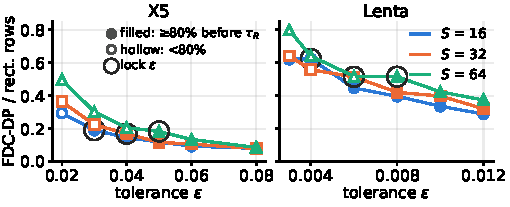
\includegraphics[width=\columnwidth]{../latex_acm/figures/fig5_eps_curve.pdf}
\caption{(Figure 2 of the paper until revision r7.) Rows ratio FDC-DP / matched rectangle, both time-uniform, against $\eps$ (block G1, post hoc, descriptive; the same 200 fresh streams at every $\eps$; pointwise 95\% CIs within $\pm 0.01$). Hollow: fewer than 80\% of rectangle streams certify before the horizon; these endpoint ratios are horizon-sensitive. Circled: the lock-v10 $\eps$ (descriptive at X5 $S = 64$).}
\label{fig:epscurve}
\Description{Two panels, X5 and Lenta, with one line per segment count (16, 32, 64). The ratio of rows needed by the joint certificate to rows needed by the matched rectangle generally falls as the tolerance grows, from 0.29--0.50 to about 0.08 on X5 and from 0.62--0.80 to 0.29--0.37 on Lenta.}
\end{figure}

\textbf{G2: knapsack costs, and what branch-and-bound buys.} Every lock-v10 class is a cardinality budget, under which the inner maximisation is a sort. G2 runs on the development halves (seeds 950--999, 50 streams per $\eps$) and gives each segment an integer treatment cost from 1 to 24 ($\kappa_s = \max(1, \mathrm{rint}(8 c_s/\bar c))$, no upper cap), with budgets $\lfloor b_q \sum_s \kappa_s \rfloor$. On X5 the costs are simulated, $c_s = \exp(0.5 z_s)$ with seeded normal $z_s$; on Lenta, $c_s$ is the segment's development mean of the 15-day discount depth, a covariate-only promotion-cost proxy. The rule reads no outcome, and neither cost is a measured campaign cost. Table~\ref{tab:g2} shows that scheme (b) and scheme (a) give the same $\Npen$ on every one of the 1,800 paired streams of the 36 settings (geometric-mean ratio 1.000), with 0--8 branch-only certification events per row among 4,500 problem instances (50 streams $\times$ 6 $\eps$ $\times$ 15 problems), no node-limit hit and at most 1.8\,s per checkpoint at $S = 64$. FDC-DP needed 0.09--0.67 of RECT-BF-DP's rows wherever the rectangle passed the 80\% criterion. Scheme (a) is already statistically sound, so branch-and-bound is an exact-decision refinement that recovers the completed-search decision and occasionally an extra certificate, with no $N_{80}$ saving in these runs. The certificate's advantage thus carries over to heterogeneous knapsack constraints on real outcome pools, as a descriptive development-half result.

% generated by writing/scripts/gen_r6_blockG_tables.py from exp/results/full/v10_posthoc_G/summary.json; do not edit by hand

\begin{table}[t]
\caption{\textbf{Block G2: heterogeneous knapsack costs} (post hoc, descriptive, development halves only; seeds 950--999, 50 streams per $\eps$, six $\eps$ per row; X5 costs simulated, Lenta costs a covariate proxy). (b)/(a): range over $\eps$ of the geometric-mean $\Npen$ ratio of branch-and-bound to min--max. B-only: branch-only certification events (problems certified by (b) but not (a)) among 4,500 problem instances (50 streams $\times$ 6 $\eps$ $\times$ 15 problems). vs RECT: range of FDC-DP(b)/RECT-BF-DP over the $\eps$ at which RECT-BF-DP reaches 12 of 15 before $\tau_R$ on at least 80\% of streams (--: none). Max s: largest certification time per checkpoint. No node-limit hit; no false stream.}
\label{tab:g2}
\small
\begin{tabular}{@{}llllrr@{}}
\toprule
Table & $S$ & (b)/(a) & vs RECT & B-only & Max s \\
\midrule
X5 & 16 & 1.000--1.000 & 0.09--0.25 & 8 & 0.11 \\
X5 & 32 & 1.000--1.000 & 0.09--0.22 & 4 & 0.45 \\
X5 & 64 & 1.000--1.000 & 0.11--0.18 & 4 & 1.56 \\
Lenta & 16 & 1.000--1.000 & 0.36--0.67 & 8 & 0.17 \\
Lenta & 32 & 1.000--1.000 & 0.39--0.63 & 3 & 0.45 \\
Lenta & 64 & 1.000--1.000 & 0.44--0.60 & 0 & 1.78 \\
\bottomrule
\end{tabular}
\end{table}


\textbf{G3: stronger rivals.} G3 reruns the six lock-v10 cells on fresh evaluation seeds 38600--38799 at the same 20 checkpoints against two further rivals (Table~\ref{tab:g3}). RECT-HG-DP replaces the Bennett cell radii by exact-hypergeometric ones and is valid at the checkpoints only (CP), because a fixed-time exact quantile radius does not inherit the time-uniform proof (Remark 4.2); it is therefore an additional exact-inversion comparison, weaker in guarantee than the time-uniform matched rectangle, and not a matched time-uniform test. HC-WoR-DP is time-uniform (TU) and was tuned over eight configurations on development seeds. The RECT-BF-DP-TU ratios replicate lock v10 within 0.003. The additional rivals shift the ratios by about 0.035 at most (0.0353, RECT-HG-DP on X5 at $S = 16$). Neither is uniformly stronger than the matched rectangle: at X5 $S = 64$ the tuned HC-WoR-DP gives 0.152 against 0.182, because it reaches 12 of 15 before $\tau_R$ on no stream. All three rivals have a mean exhausted-control fraction of 1 in every Lenta cell, so the Lenta cells remain stopping comparisons at the rivals' control-pool exhaustion. No tested rival closes the gap, and the claim still covers only the named rivals.

% generated by writing/scripts/gen_r6_blockG_tables.py from exp/results/full/v10_posthoc_G/summary.json; do not edit by hand

\begin{table}[t]
\caption{\textbf{Block G3: stronger rivals at the lock-v10 cells} (post hoc, descriptive; fresh evaluation seeds 38600--38799, 200 streams per cell). Paired geometric-mean $\Npen$ ratio of TU-FDC-DP(b) to each rival, one-sided UB95 in parentheses. RECT-HG-DP: exact-hypergeometric cell radii with the same knapsack worst gap. HC-WoR-DP tuned: best of eight configurations on development seeds, selected before any G3 evaluation row. Guarantee strength on the 20 checkpoints: RECT-BF-DP-TU TU on the frozen schedule; RECT-HG-DP CP only (a checkpoint-valid exact inversion, not a time-uniform rectangle); HC-WoR-DP TU.}
\label{tab:g3}
\small
\begin{tabular}{@{}llrlll@{}}
\toprule
Table & $S$ & $\eps$ & RECT-BF-DP-TU & RECT-HG-DP & HC tuned \\
\midrule
X5 & 16 & 0.03 & 0.188 (0.191) & 0.223 (0.227) & 0.200 (0.204) \\
X5 & 32 & 0.04 & 0.168 (0.170) & 0.168 (0.170) & 0.168 (0.170) \\
X5 & 64 & 0.05 & 0.182 (0.185) & 0.187 (0.188) & 0.152 (0.153) \\
Lenta & 16 & 0.004 & 0.629 (0.634) & 0.633 (0.636) & 0.632 (0.636) \\
Lenta & 32 & 0.006 & 0.518 (0.521) & 0.519 (0.523) & 0.518 (0.521) \\
Lenta & 64 & 0.008 & 0.513 (0.513) & 0.513 (0.513) & 0.513 (0.513) \\
\bottomrule
\end{tabular}
\end{table}


\clearpage
\section{Localised union ledgers (development only, negative)}\label{app:localised}

Two localised or prior-weighted replacements for FDC-DP's uniform union were built and replayed after the r6 reviews, and a third was examined only through a Gaussian calculation; neither replayed ledger read fewer rows than FDC-DP on the development halves. The question was whether the union cost of Section 6.5 of the paper ($\beta_J/\beta_C = 4.50$ at $S = 64$) can be lowered by a ledger that spends less of $\dmain$ on challengers far from a plausible optimum. Each construction keeps FDC-DP's Chernoff event and replaces the uniform allocation by frozen weights $w_q(\pi) \ge 0$ with $\sum_{\pi \in \Pi_q} w_q(\pi) \le 1$, so the union still sums to $\dmain$ and the event holds with the challenger-dependent exponent $\beta(q,\pi) = \ln(QK/\dmain) + \ln(1/w_q(\pi))$. (1) \emph{FDC-PW} puts its weight on Hamming shells around a reference policy $\mathrm{ref}_q$, the knapsack argmax of the frozen covariate-only score model of Section 6.5, so no outcome is read; it tries two candidate centres, the empirical argmax and $\mathrm{ref}_q$, and runs scheme (b). The code's default Hamming-ball centres were not run. (2) \emph{FDC-LS} puts half its weight uniformly and half on Hamming shells around the unknown optimum $\pi^*_q$, and evaluates the challenger-dependent exponent exactly by a knapsack DP with a flip-count state (scheme (a)). Its nearest shell has $\beta_1 = 15.01$ and its far shells pay $\beta_J + \ln 2 = 53.03$, against $\beta_J = 52.34$ at $S = 64$. (3) A thresholded-sum event, one Chernoff event for $\sum_s (|\xi_s| - c_s)_+$, was examined only through a Gaussian calculation, which showed no gain where the width binds, so it was not built. FDC-PW and FDC-LS are time-uniform on the frozen block grid like TU-FDC-DP. The code is \texttt{exp/code/dsswm/baselines/fdc\_\{pw,ls\}.py} with \texttt{dsswm/envs/pw\_reference.py}, and the tests \texttt{exp/code/dsswm/tests/test\_fdc\_\{pw,ls\}.py} check the weight sums, the shell-counting and flip-state DPs against enumeration, the reduction to FDC-DP under uniform weights and the family-wise error on toy Monte Carlo streams. These are tested constructions, not formal results of the paper.

% generated by writing/scripts/gen_r6d_s20.py; do not edit by hand
\begin{table}[H]
\caption{\textbf{Localised ledgers against FDC-DP} (development halves only; post hoc, descriptive). Paired geometric mean of $\Npen$, variant / TU-FDC-DP(b), on the same development streams (seeds 950--999) and tolerance grid as the block-G1 development cells. Ratio: range over the $\eps$ with all 50 streams (``complete''). Stopped: streams present in the $\eps$ at which the run was stopped, not reported as ratios. No false certificate in any row. Generated by \texttt{writing/scripts/gen\_r6d\_s20.py} from \texttt{exp/results/pilots/fdc\_pw/}.}
\label{tab:s20}
\footnotesize
\setlength{\tabcolsep}{3pt}
\begin{tabular}{@{}llllr@{}}
\toprule
Log, $S$ & Variant & Complete $\eps$ & Ratio & Stopped \\
\midrule
X5, 16 & FDC-PW & 6 of 6 & 1.038--1.086 & -- \\
X5, 16 & FDC-LS & 6 of 6 & 1.015--1.046 & -- \\
X5, 32 & FDC-PW & 6 of 6 & 1.011--1.050 & -- \\
X5, 32 & FDC-LS & 6 of 6 & 1.011--1.034 & -- \\
X5, 64 & FDC-PW & 2 of 6 & 1.004 & 33 \\
X5, 64 & FDC-LS & 0 of 6 & -- & 3 \\
Lenta, 16 & FDC-PW & 6 of 6 & 1.008--1.067 & -- \\
Lenta, 16 & FDC-LS & 6 of 6 & 1.000--1.029 & -- \\
Lenta, 32 & FDC-PW & 1 of 6 & 1.004 & 14 \\
Lenta, 32 & FDC-LS & 6 of 6 & 1.004--1.016 & -- \\
Lenta, 64 & FDC-PW & 1 of 6 & 1.000 & 46 \\
Lenta, 64 & FDC-LS & 0 of 6 & -- & 3 \\
\bottomrule
\end{tabular}
\end{table}


On every complete cell the localised ledgers read 1.00 to 1.09 times FDC-DP's rows, and no geometric mean fell below 1 (Table~\ref{tab:s20}). FDC-PW gave 1.000--1.086 and FDC-LS 1.000--1.046. Coverage is uneven at large $S$, where the exact shell DPs are slow. FDC-PW is complete at all six $\eps$ at X5 $S = 16, 32$ and Lenta $S = 16$, at the two smallest $\eps$ at X5 $S = 64$ and at the smallest $\eps$ at Lenta $S = 32$ and 64; its runs at the next $\eps$ were stopped after 33, 14 and 46 streams. FDC-LS is complete at $S = 16$ and 32 on both logs and was stopped at $S = 64$ after 3 streams at the smallest $\eps$ on each log, with ratio 1.000 on all of them. Localisation therefore bought no rows wherever it was measured.

The diagnostics place the cause in the near-tie geometry of these tables rather than in the choice of weights. The frozen-score reference is close to the optimum in value but far from it in policy space: at $S = 64$ its Hamming distance to the true development optimum is 10--34 segments on X5 and 6--32 on Lenta, with value gaps of 0.004--0.014 and 0.001--0.005 against tolerances of 0.02--0.08 and 0.003--0.012. Weights centred on it therefore favour challengers that never bind. Shell localisation around $\pi^*_q$ lowers the exponent only at small Hamming distance, whereas the challengers that maximise $\hat\Delta + W$ differ from the centre in many near-tie segments; the true-gap census of S12 (3,076 of 3,347 X5 development pairs $\eps$-optimal) and FDC-LOC's $\hat\beta/\beta_J = 1.000$ on X5 show the same geometry. For the examined thresholded-sum construction, whose centre is chosen from the data, the union-free event we considered controls $\sum_s |\xi_s|$ rather than $\sum_s (\xi_s)_+$, and under Gaussian cell errors the per-segment means of these differ by a factor of two ($0.80\sigma$ against $0.40\sigma$); this heuristic is why construction (3) was not built. The null result is thus explained by where the binding challengers lie, not by a defect of the tested weights.

This section is descriptive and narrow. It used development halves only, read no evaluation row and involved no lock, and it replayed two constructions and examined a third analytically on two near-tie tables. It is not a lower bound: Peace-style Gaussian-width thresholds over the knapsack class and chaining were not tried, and a better complexity-dependent certificate is not ruled out. The work is recorded in \texttt{plan/v11\_plan.md}; the Hamming distances and value gaps come from \texttt{gen\_r6d\_s20.py --diag}. What it does show is that FDC-DP pays the union cost in full on these tables and still saves rows because $\meff$ exceeds it.

\clearpage
\section{Lock v11: Open Bandit confirmatory block}\label{app:v11}

Lock v11 is the first confirmatory block whose evaluation outcomes informed nothing in its design, and it answers the objection that every earlier confirmatory table had been replayed before. It is unrelated to the development notes \texttt{plan/v11\_plan.md} of S20, which predate it and share only the version number. Its plan (\texttt{plan/v11\_obd\_plan.md}) was committed alone before any v11 development stream; its development report is \texttt{plan/v11\_dev\_report.md}; the locked addendum is \texttt{plan/prereg\_lock\_v11\_addendum.json} (canonical sha256 \texttt{4ee73391\ldots 629963}, code freeze \texttt{1741ebcf}, lock commit \texttt{91606679}), reviewed by an external reviewer in two rounds (verdict ``lock'' in round 2). The block is a direct test of FDC-DP against the time-uniform matched rectangle under the lock-v10 protocol, so the section first states the data and blinding, then the design and rules, then the result.

\begin{table*}[t]
\caption{\textbf{Lock v11, every comparison} (Open Bandit Dataset, \texttt{random/all} evaluation half, 200 fresh paired streams, seeds 39000--39199, $\eps = 3\cdot 10^{-4}$, $K = 40$). Ratio = paired geometric mean of $\Npen$ (first / second method) with two-sided 95\% CI and one-sided UB95 (paired percentile bootstrap, $B = 10^4$, seed 42, one resample matrix). F / T / S = \% of streams on which the first method stops earlier / at the same checkpoint / later. Dev = the same statistic on the 50 development streams of the selected $\eps$ (seeds 950--999), UB95 in parentheses. Decision rule: UB95 of the primary row $< 0.90$, no false TU-FDC-DP(b) stream over the whole run, replica pass; verdict \texttt{positive\_result\_achieved}.}
\label{tab:v11ratios}
\small
\setlength{\tabcolsep}{4pt}
\begin{tabular}{@{}llllll@{}}
\toprule
Comparison & Role & Ratio [95\% CI] & UB95 & F / T / S & Dev (UB95) \\
\midrule
\textbf{TU-FDC-DP(b) / RECT-BF-DP-TU} & primary & 0.817 [0.808, 0.826] & 0.824 & 99.5 / 0.5 / 0 & 0.825 (0.840) \\
TU-FDC-DP(b) / HC-WoR-DP (tuned) & descr. & 0.822 [0.814, 0.830] & 0.829 & 100 / 0 / 0 & 0.828 (0.840) \\
TU-FDC-DP(b) / RECT-HG-DP & descr. & 0.826 [0.817, 0.834] & 0.833 & 98.5 / 1.5 / 0 & 0.840 (0.851) \\
RECT-BF-DP-TU / HC-WoR-DP (tuned) & descr. & 1.006 [1.002, 1.011] & 1.010 & 1 / 93 / 6 & 1.003 (1.010) \\
RECT-BF-DP-TU / RECT-HG-DP & descr. & 1.011 [1.006, 1.016] & 1.015 & 0 / 91.5 / 8.5 & 1.018 (1.028) \\
\bottomrule
\end{tabular}
\end{table*}

\begin{table*}[t]
\caption{\textbf{Lock v11, every method} (same 200 streams). Guar.: TU fr.\ = time-uniform on the frozen schedule; TU any = time-uniform under any predictable sampling; CP = valid at the $K$ checkpoints only. False: streams with any false certificate over the whole run to 15 of 15 (one-sided 95\% Clopper--Pearson bound). Rows: geometric-mean $\Npen$ ($\tau_R$ = 688,159 rows). $N_{80}/\tau_R$: geometric mean. $<\tau_R$: \% of streams reaching 12 of 15 strictly before $\tau_R$; 15/15: \% reaching 15 of 15. Exhausted: mean fraction of all / control / treatment pools exhausted at $N_{80}$. B\&B: branch-and-bound calls / branch-only certifications / node-limit hits (scheme (b)).}
\label{tab:v11methods}
\small
\setlength{\tabcolsep}{3.5pt}
\begin{tabular}{@{}lllrrrrll@{}}
\toprule
Method & Guar. & False (UB) & Rows & $N_{80}/\tau_R$ & $<\tau_R$ & 15/15 & Exhausted & B\&B \\
\midrule
TU-FDC-DP(b) & TU fr. & 0 (.015) & 499.3k & 0.726 & 100 & 100 & 0.00 / 0.00 / 0.00 & 105,348 / 219 / 0 \\
RECT-BF-DP-TU & TU fr. & 0 (.015) & 611.1k & 0.888 & 94 & 100 & 0.06 / 0.06 / 0.06 & --- \\
HC-WoR-DP (tuned) & TU any & 0 (.015) & 607.3k & 0.882 & 97 & 100 & 0.03 / 0.03 / 0.03 & --- \\
RECT-HG-DP & CP & 0 (.015) & 604.6k & 0.879 & 100 & 100 & 0.00 / 0.00 / 0.00 & --- \\
\bottomrule
\end{tabular}
\end{table*}


\textbf{Data and blinding.} The Open Bandit Dataset (Saito et al., NeurIPS 2021 Datasets and Benchmarks; ZOZOTOWN, CC BY 4.0) logs fashion recommendations in three positions under a uniform-random logging policy over 80 items (propensity 1/80) with a binary click outcome. Only \texttt{random/all/all.csv} (1,374,327 rows) was read; \texttt{random/men}, \texttt{random/women} and the Thompson-sampling logs stay unread. A row is in the development half iff \texttt{int(sha256(f"\{salt\}|open\_bandit|\{row\_id\}")[:8], 16) / 2**32 < 0.5} with salt \texttt{dsswm-obd-2026-10-05}, where \texttt{row\_id} is the CSV's unnamed first column. The split gives 686,168 development and 688,159 evaluation rows. It was written before any click was read: evaluation outcomes went to a separate read-only file, and only label statistics (position and item shares) of the evaluation half were computed at split time. Before the lock no v11 code opened or hashed an evaluation outcome; the first development runs hashed the bytes of the evaluation label file without deserialising it, and after the first lock review both evaluation hashes come from the hash-bound provenance record. The evaluation half was replayed in one registered block, through a gated reader that appends an access-log line before reading; the access log has three records (the main run at 15:12:18, then the prespecified ten-seed replica and the analysis), and the run was sealed alone (commit \texttt{81ba8691}; rows and run record \texttt{6972e18f}) before the replica check and the analysis. The blinding thus rests on code paths and git history, not on proof against unrecorded access.

\textbf{Frozen design.} Everything below was fixed on the development half (Table~\ref{tab:v11design}). Segments are the user-feature cells uf0 $\times$ uf3, with cells under 2\% of development rows merged into their uf0 ``other'' cell, giving $S = 9$; unseen pairs route to that cell (no evaluation row needed the fallback). Arm 1 shows a uniformly random item among the 40 with the highest development click rate, arm 0 one of the other 40, so each cell mean is the finite-population click rate of a group policy in a segment. Treating segment $s$ costs $\kappa_s = \max(1, \mathrm{round}(8 S w_s^{\text{dev}}))$, from 2 to 26, and the 15 budgets $\lfloor b_q \sum_s \kappa_s \rfloor$, $b_q = 0.10, \dots, 0.80$, define knapsack classes over the 512 policies; policy values use the evaluation weights. Every method reads the same frozen outcome-free 50/50 schedule, with $\delta = 0.05$ and $K = 40$ log-spaced checkpoints from 5,000 rows to $\tau_R = 688{,}159$. The design is therefore the lock-v10 protocol with knapsack costs and a finer grid.

\begin{table}[H]
\caption{\textbf{Lock v11 frozen design.} Segments (uf0 $\times$ uf3 cells, cells under 2\% of development rows merged into their uf0 ``other'' cell, ordered by development size), development and evaluation traffic shares $w_s$, and treatment cost $\kappa_s = \max(1, \mathrm{round}(8 S w_s^{\text{dev}}))$ (control costs 0). Budgets $\lfloor b_q \sum_s \kappa_s \rfloor$ for $b_q = 0.10, 0.15, \dots, 0.80$: 7, 10, 14, 17, 21, 24, 28, 31, 35, 39, 42, 46, 49, 53, 56. Arms: the 40 items with the highest development click rate (arm 1) against the other 40 (arm 0); an arm shows a uniformly random item of its group.}
\label{tab:v11design}
\footnotesize
\setlength{\tabcolsep}{4pt}
\begin{tabular}{@{}rrrr@{}}
\toprule
Segment & $w_s$ (dev) & $w_s$ (eval) & $\kappa_s$ \\
\midrule
1 & 0.367 & 0.366 & 26 \\
2 & 0.193 & 0.194 & 14 \\
3 & 0.193 & 0.192 & 14 \\
4 & 0.057 & 0.057 & 4 \\
5 & 0.048 & 0.048 & 3 \\
6 & 0.043 & 0.044 & 3 \\
7 & 0.035 & 0.035 & 3 \\
8 & 0.032 & 0.032 & 2 \\
9 & 0.031 & 0.031 & 2 \\
\bottomrule
\end{tabular}
\end{table}


\textbf{Methods.} The primary method is TU-FDC-DP(b), the lock-v10 construction (scheme (b), node limit $2\cdot 10^5$, $\lambda$ grid ratio $2000^{1/160}$, $\dmain = 0.045$, $\dvar = 0.005$) with the $K = 40$ grid as block points. The governing rival is RECT-BF-DP-TU, the parameter-free time-uniform matched rectangle with boxes and the exact worst-gap DP. Two descriptive rivals complete the block: HC-WoR-DP, tuned on development streams by the block-G3 rule over eight configurations, and RECT-HG-DP, the exact-hypergeometric rectangle at level $\delta/(2SAK)$, which is valid at the checkpoints only (CP). Plug-in rules were not run, following the paper's restriction of the headline to methods with proven guarantees. The comparison is therefore at matched time-uniform strength for the primary pair and descriptive otherwise.

\textbf{$\eps$ rule and threshold.} The rival-success rule of lock v10 chose $\eps$ on 50 development streams (seeds 950--999) without reading FDC-DP: the smallest grid value at which the better of RECT-BF-DP-TU and the tuned HC-WoR-DP reaches 12 of 15 strictly before $\tau_R$ on at least 40 of 50 streams (Table~\ref{tab:v11eps}). It selected $\eps = 3\cdot 10^{-4}$, about 8.6\% of the development click rate of 0.350\% and 8.7\% of the evaluation rate of 0.343\%. On the evaluation truth 15.1\% of feasible policies are $\eps$-optimal on average and no problem has the all-control policy $\eps$-optimal, so the frontier is not trivial at this tolerance. A feasibility pilot at $K = 20$ had found that the rectangle never certified at $3\cdot 10^{-4}$; with $K = 40$ it certifies at checkpoint 38 of 40, which moved the selection from the expected $5\cdot 10^{-4}$ to $3\cdot 10^{-4}$ as a consequence of the pre-stated $K$ change. The threshold rule, written before any v11 development stream, is THRESH $= \min(0.90, \mathrm{UB95}_{\text{dev}} + 0.10)$; the development cell gave 0.825 (UB95 0.840), so THRESH $= 0.90$. The confirmatory statistic is the paired geometric-mean ratio of $\Npen$, TU-FDC-DP(b) / RECT-BF-DP-TU, over 200 fresh streams (seeds 39000--39199), and the block is positive iff its UB95 is below 0.90, no TU-FDC-DP(b) stream has a false certificate over the whole run to 15 of 15 and the replica check passes. Both the tolerance and the threshold were thus fixed by rules that never saw an evaluation outcome.

\begin{table}[H]
\caption{\textbf{Lock v11 $\eps$ rule and rival tuning} (development half, 50 streams, seeds 950--999, $K = 40$). Top: the rule's trace. Each rectangle's entry is successes (12 of 15 strictly before $\tau_R$) / geometric-mean $\Npen$; the dev-best (lower geometric mean) must succeed on at least 40 of 50 streams, and the smallest qualifying $\eps$ of the grid is selected, so the trace stops at its first entry. FDC-DP rows never enter the rule. Bottom: the tuned HC-WoR-DP configuration (schedule \texttt{nstar}; $c$, target fraction) at each grid $\eps$, its successes, geometric-mean $\Npen$ and false streams.}
\label{tab:v11eps}
\footnotesize
\setlength{\tabcolsep}{2.5pt}
\begin{tabular}{@{}lllll@{}}
\toprule
$\eps$ & RECT-BF-DP-TU & HC-WoR-DP (tuned) & dev-best & qualifies \\
\midrule
$3\cdot 10^{-4}$ & 48 / 607,878 & (0.5, 0.6) 47 / 606,345 & HC-WoR-DP & yes (selected) \\
\midrule
$\eps$ & HC config & successes & geo.\ $\Npen$ & false \\
\midrule
$3\cdot 10^{-4}$ & (0.5, 0.6) & 47 / 50 & 606,345 & 0 \\
$5\cdot 10^{-4}$ & (0.5, 0.6) & 50 / 50 & 517,206 & 0 \\
$7.5\cdot 10^{-4}$ & (0.5, 0.4) & 50 / 50 & 417,342 & 0 \\
$10\cdot 10^{-4}$ & (0.5, 0.4) & 50 / 50 & 351,524 & 0 \\
$15\cdot 10^{-4}$ & (0.5, 0.4) & 50 / 50 & 251,286 & 0 \\
\bottomrule
\end{tabular}
\end{table}


\textbf{Result.} The verdict is positive (Table~\ref{tab:v11ratios}). TU-FDC-DP(b) needed 0.817 [0.808, 0.826] times the rows of RECT-BF-DP-TU, UB95 0.824 against 0.90, was faster on 99.5\% of streams, tied on 0.5\% and slower on none, and made no false certificate; no method made one (Clopper--Pearson bound 0.015 each). The replica check passed (R1: the first ten seeds re-run in an independent process give identical canonical rows; R2 and R2b: identical schedule and arrival digests across the four methods on all 200 streams). Against the descriptive rivals the ratio is 0.822 (tuned HC-WoR-DP, faster on every stream) and 0.826 (RECT-HG-DP, CP), and the three rivals lie within 1.1\% of one another (RECT-BF-DP-TU / HC-WoR-DP 1.006, RECT-BF-DP-TU / RECT-HG-DP 1.011). The development estimates were 0.825, 0.828 and 0.840, so the evaluation half reproduced, and slightly exceeded, the development effect. The result therefore confirms the lock-v10 ordering on a log that no earlier test had touched.


\textbf{Where the rows go.} TU-FDC-DP(b) certified 12 of 15 problems after a geometric mean of 72.6\% of the evaluation half, against 88.8\% for RECT-BF-DP-TU, 88.2\% for HC-WoR-DP and 87.9\% for RECT-HG-DP (Table~\ref{tab:v11methods}). Stopping is concentrated on a few late checkpoints: TU-FDC-DP(b)'s $N_{80}$ is 415,272, 471,164, 534,578 or 606,527 rows (60.3\%, 68.5\%, 77.7\% and 88.1\% of the table, checkpoints 35--38) on 11, 87, 101 and 1 streams, whereas RECT-BF-DP-TU stops at 606,527 rows (88.1\%) on 188 streams and reaches $\tau_R$ on the other 12. TU-FDC-DP(b) thus reached 12 of 15 strictly before $\tau_R$ on every stream, against 94\% for the governing rival, and had no exhausted pool at its stopping point on all 200 streams; both methods had none on 188 streams, and on the 12 horizon streams every pool of the rectangle was exhausted, which gives its mean exhausted fraction of 0.06. The lock-v10 condition for a pre-exhaustion width claim requires both methods' exhausted fractions to be zero (S17), so it is not met at block level; the v11 decision rule does not use it, and the verdict is unaffected. Two descriptive readings, both computed after the analysis with the same bootstrap ($B = 10^4$, seed 42), bound how much the horizon matters. On the 188 streams where neither method had an exhausted pool, the ratio is 0.821 (UB95 0.829), so the penalty at $\tau_R$ does not drive the result. At the full-frontier time (15 of 15, a secondary endpoint), the geometric means are 572,301 and 670,998 rows and the ratio is 0.853 (UB95 0.859), but the rectangle reaches 15 of 15 only at $\tau_R$ on 160 of 200 streams, so that ratio is horizon-sensitive and is not the registered endpoint. Branch-and-bound ran 105,348 times, produced 219 certifications that scheme (a) alone would not have issued, and never hit the node limit; these change no $N_{80}$ comparison by themselves. Because the checkpoints are log-spaced, one step changes a stream's ratio by a factor of about 1.13, so the narrow interval reflects a near-discrete endpoint rather than a large effect.

\textbf{Disclosures.} (i) The arm grouping and the choice of the uf0 $\times$ uf3 segmentation among the feasibility candidates used development outcomes; the evaluation half was used once, after the lock, but the evaluation uplift gap may shrink by selection. A feasibility holdout froze only the item groups and recomputed segments and costs on its replay half, so it was not a rehearsal of the full frozen-design transfer. (ii) The split is row-level: 3.3\% of development rows share an exact timestamp with an evaluation row (multi-position impressions), and user ids are absent, so repeat users can fall in both halves; the halves are therefore not independent, and the log gives no quantitative bound on their dependence. (iii) $K = 40$, not the 20 of locks v7--v10, is a pre-stated change for ratio resolution, paid for in both ledgers. (iv) Costs are traffic shares, not monetary prices; the log documents no price field. (v) HC-WoR-DP was tuned on the same development streams that the $\eps$ rule used, which is selection-optimistic for HC-WoR-DP; RECT-HG-DP has checkpoint strength only. (vi) The base click rate is 0.35\%, and each segment-arm cell holds roughly 10 to 700 clicks per half. (vii) The development block was regenerated once after the first lock review fixed the evaluation gate; all 2,450 regenerated rows reproduce the first run exactly, and the gate files were rewritten once for that reason only. (viii) Inference is conditional on this finite evaluation table and describes replay variation within it. (ix) The provenance record's \texttt{split\_created\_utc} (03:26 UTC, 14:26 local time) records when that record was last rewritten; the split files themselves are dated 14:01, about 25 minutes earlier, and predate the feasibility pilot. (x) The frozen evaluation module still exports \texttt{verify\_eval\_bytes}, which hashes the evaluation bytes without an authorisation check of its own; the registered reader calls it only after authorisation and logging, and because the file is lock-bound the limitation is documented here rather than repaired. (xi) \texttt{v11\_analysis.json} labels every method, including RECT-HG-DP, \texttt{validity: rigorous}; RECT-HG-DP's guarantee is checkpoint strength (CP), as stated in this section. None of (ix)--(xi) touches an outcome. The claim of Section 6.6 therefore covers the named rectangle constructions on this one log.

\section{Paragraphs moved from the paper in revision r7}\label{app:moved}

Revision r7 added the fresh-log test (Section 6.6 of the paper, S21) and paid for it by moving the paragraphs below out of Sections 5 and 6, together with Figure 2 (now Figure~\ref{fig:epscurve} in S19). Each paragraph is reproduced from revision r6d, apart from cross-references and one scope correction made in revision r7b (the block G sentence on localised ledgers now gives the corrected statement; the superseded r6d wording is quoted in the errata index, S14), and the paper keeps a shortened version of each with the same claim. No number changed.

\textbf{Section 5, guaranteed rivals (X5 families).} The X5 test's primary families are the same rectangles, with plans tuned on X5 development seeds (7 candidates for RECT-ck-HG, 63 for HC-WoR), and two PJC members. The residual-pool member (best of 17) estimates from residual pools as RAGE does, and the selected member has no boundary. The menu member (best of 10) keeps all data and chooses a control share of 0.4 or 0.5 at one boundary. Its union over menu paths is charged in full (supplement S7).

\textbf{Section 6.3, real-log adaptation.} On the two real logs adaptation had little to offer, so the registered phased tests bound a cost rather than show a win. At 77 monitoring times on X5, TU-FDC's ratio is 0.985 [0.977, 0.994] (UB95 0.992) against the residual-pool PJC with its own 77-time ledger and 1.004 [0.997, 1.010] (UB95 1.009) against its time-uniform form. It thus matches PJC within the registered 5\% margin, which had left only 0.034 of development headroom; X5 is the only log with a confirmatory non-inferiority test, and on Criteo the descriptive ratios are 0.997 and 1.000 (supplement S12). The selected X5 PJC does not adapt, and the menu member chose 50/50 on every stream. In a post-hoc block of 64 adaptive joint certificates per log, every member was slower than FDC-BF (best 0.943 on X5, 0.951 on Criteo; supplement S8), because near-equal arm variances make 50/50 nearly variance-optimal, so the real-log tests say little about adaptation.

\textbf{Section 6.3, semi-synthetic regime.} \textbf{Where adaptation can help.} A semi-synthetic block keeps the logs' segments, pools and arrival schedules but sets very unequal arm rates (supplement S11; post hoc, descriptive). There, adaptive joint certificates can beat frozen 50/50 FDC-BF: on the Criteo-structured asymmetric regime they read 8--11\% fewer rows (FDC-BF/method 1.087--1.127). A follow-up block gives every method on a stream the same independent pilot of 250 or 1,000 draws per cell, as from a prior campaign. At equal pilot information, frozen pilot-Neyman FDC-BF needed 0.90--0.98 times the rows of each tested reset and menu design in all four regimes. All 128 such comparisons have 95\% intervals below 1, also with the pilot charged in full to both sides, so equal information favours the frozen plan everywhere tested.

\textbf{Section 6.3, charged pilot.} A different comparison charges the pilot to the frozen plan alone and pits it against adaptive designs that use none. On Criteo-sized tables the pilot is at most 0.26\% of $\tau_R$, and the point estimates still favour the frozen plan (0.89--0.99), although one of eight intervals includes 1. On X5-sized tables a pilot of 4.5\% or 18\% of $\tau_R$ reverses this comparison (1.08--1.67); in point estimates it breaks even only when one pilot serves 2.1 to 25.5 runs, that is 3 to 26 whole runs. The adaptive designs were compared at checkpoint strength and not retuned with a pilot. An informed frozen plan therefore beats these adaptive implementations at equal information, while against pilot-free adaptation on small tables it pays off only when its pilot already exists or is shared across runs.

\textbf{Section 6.4, exact rectangle.} The exact rectangle beats the matched one (predicted rows ratio 0.75, observed 0.775; App.~B of the paper) only because exact test inversion is tighter than any Chernoff radius.

\textbf{Section 6.4, ablations.} In two ablations neither a tighter cell inequality nor the tested ledger localisation moved the saving much (supplement S12). An exact hypergeometric cell envelope, valid and never wider, needed 0.969 (UB95 0.990) times FDC-BF's rows on Criteo and 0.944--0.976 on X5 development streams, because at certification the two bounds differ only in third-order terms. A gap-weighted, still valid localisation of the union gave 0.925 (UB95 0.949) and 1.000, because most (problem, policy) pairs are near-ties, and even an invalid oracle that knows the true gaps reaches only 0.81. Both ablations failed go criteria fixed before their development runs, so the tested localisation changes little on these tables.

\textbf{Section 6.5, block G.} A post-hoc block G addresses three objections (supplement S19). First, on the tested grid the rule-selected $\eps$ gives the largest ratio among tolerances at which the rectangle passes the 80\% pre-horizon criterion; the ratio generally falls as $\eps$ grows, to 0.08--0.09 on X5 and 0.29--0.37 on Lenta at the largest $\eps$, and is 0.09--0.18 and 0.34--0.45 where the rectangle passes that criterion and is unpinned (Figure~\ref{fig:epscurve} in S19). Second, on development halves (50 streams per $\eps$) with simulated or proxy heterogeneous costs, FDC-DP needed 0.09--0.67 of the rectangle's rows wherever it passed that criterion. Branch-and-bound left $N_{80}$ unchanged on every stream of all 36 knapsack settings, and in lock v10, where every class is a cardinality budget, it changed $N_{80}$ on 0--1 of 200 streams per cell, so it is an exact-decision refinement rather than a source of speed. Third, a checkpoint-valid exact-hypergeometric rectangle, weaker in guarantee than the time-uniform rivals, and a development-tuned betting rectangle moved the lock-cell ratios by about 0.035 at most. The union cost grows with the class: $\beta_J/\beta_C$ is 1.47, 1.86, 2.75 and 4.50 at $S$ = 9, 16, 32 and 64, so to leading order the joint width wins only while $\meff$ exceeds that ratio. Two localised union ledgers read no fewer rows on development halves, and a Gaussian diagnostic rejected a third before it was built (supplement S20), so FDC-DP pays this cost in full.

\textbf{Section 6.6, robustness.} The ordering persisted over the tested settings of $\delta$, $\dvar$, $K$, the $\lambda$ grid and the replanning batch (supplement S10; post hoc, development halves). FDC-BF/rectangle stayed within 0.27--0.36 on X5 and 0.50--0.69 on Criteo, with no false certificate in 5,500 runs, which says nothing outside that one-at-a-time grid.

\textbf{Section 6.6, Hillstrom and other descriptive context.} A three-arm log gives the same ordering with a smaller margin, descriptively, because an earlier analysis had exposed the cell means of Hillstrom's e-mail experiment (Hillstrom, 2008). On its evaluation half (729 policies) FDC-BF needed 0.807 (UB95 0.814) and 0.791 (UB95 0.799) times the rows of the tuned exact and betting rectangles and 0.993 (UB95 0.997) times those of the residual-pool PJC, with no false stream; 20.5\% and 31\% of the rectangles' streams reach 12 of 15 only at $\tau_R$, so these ratios are horizon-sensitive (supplement S13). On a 4,096-policy Criteo segmentation FDC-BF needs 0.546--0.547 times the rectangles' rows (supplement S3, S6). The asymptotic Qini rule (Sverdrup et al., 2025) is faster (0.46 and 0.27) but had 2 false Criteo streams of 200, so rules without a proof stay descriptive.

\section{Lock v12: descriptive replications on two further Open Bandit campaigns}\label{app:v12}

Lock v12 asks whether the lock-v11 ordering replicates on the Open Bandit Dataset's two other uniform-random campaigns, \texttt{random/women} (block A, primary) and \texttt{random/men} (block B), which no earlier step had read. Both blocks are descriptive by a gate fixed in the plan before any of their outcomes were read, so this section reports replication evidence for the direction and size of the saving, not a second confirmatory test, and no ratio is pooled with lock v11 or across campaigns. The plan (\texttt{plan/v12\_obd2\_plan.md}) was committed alone (\texttt{317619b4}, renamed and extended in \texttt{5b3eb048}) before any split, click read or development stream; the development report is \texttt{plan/v12\_dev\_report.md}; the locked addendum is \texttt{plan/prereg\_lock\_v12\_addendum.json} (canonical sha256 \texttt{9a99ef28\ldots 075c189}, code freeze \texttt{20a5e314}, lock commit \texttt{be886f1c}), reviewed by the same external reviewer in two rounds (\texttt{v12\_lock\_review\_r\{1,2\}.md}). Results are in \texttt{v12\_\{women,men\}\_analysis.json} under \texttt{exp/results/full/v12\_obd/}, summarised in \texttt{exp/results/full/v12\_summary.md}; Tables~\ref{tab:v12ratios}--\ref{tab:v12design} are generated from these files by \texttt{writing/scripts/gen\_r8\_v12\_tables.py}. The section states the data and blinding, the design and the gate, then the result and the disclosures.

\begin{table*}[t]
\caption{\textbf{Lock v12, every comparison} (Open Bandit Dataset, \texttt{random/women} and \texttt{random/men} evaluation halves, 200 fresh paired streams each). Both blocks are \emph{descriptive} by the block-status gate fixed in the plan before any of their data were read (Table~\ref{tab:v12gate}); no row carries a verdict, THRESH is not applicable, and no ratio is pooled with lock v11 or across campaigns. Ratio = paired geometric mean of $\Npen$ (first / second method) with two-sided 95\% CI and one-sided UB95 (paired percentile bootstrap, $B = 10^4$, seed 42, one resample matrix per block). F / T / S = \% of streams on which the first method stops earlier / at the same checkpoint / later. Full frontier: rows to 15 of 15 (horizon-sensitive). Uncensored subset: streams on which neither method had an exhausted pool at $N_{80}$ (pre-stated in the v12 plan). Dev = the same statistic on the 50 development streams of the selected $\eps$ (seeds 950--999), UB95 in parentheses.}
\label{tab:v12ratios}
\small
\setlength{\tabcolsep}{4pt}
\begin{tabular}{@{}llllll@{}}
\toprule
Comparison & Role & Ratio [95\% CI] & UB95 & F / T / S & Dev (UB95) \\
\midrule
\multicolumn{6}{@{}l}{\emph{A. women (seeds 39200--39399, $\eps = 7.5\cdot 10^{-4}$, 15.5\% of the development click rate; $\tau_R$ = 432,576; block status: descriptive)}} \\
\textbf{TU-FDC-DP(b) / RECT-BF-DP-TU} & headline & 0.677 [0.670, 0.684] & 0.683 & 100 / 0 / 0 & 0.719 (0.729) \\
TU-FDC-DP(b) / HC-WoR-DP (tuned) & descr. & 0.715 [0.708, 0.723] & 0.721 & 100 / 0 / 0 & 0.721 (0.731) \\
TU-FDC-DP(b) / RECT-HG-DP & descr. & 0.731 [0.723, 0.738] & 0.737 & 100 / 0 / 0 & 0.721 (0.731) \\
RECT-BF-DP-TU / HC-WoR-DP (tuned) & descr. & 1.057 [1.049, 1.066] & 1.064 & 0 / 51.5 / 48.5 & 1.002 (1.007) \\
RECT-BF-DP-TU / RECT-HG-DP & descr. & 1.080 [1.072, 1.088] & 1.086 & 0 / 33 / 67 & 1.002 (1.007) \\
TU-FDC-DP(b) / RECT-BF-DP-TU, full frontier ($N^{\text{pen}}_{100}$) & descr. & 0.726 [0.719, 0.733] & 0.732 & 100 / 0 / 0 & 0.705 (0.711) \\
TU-FDC-DP(b) / RECT-BF-DP-TU, uncensored subset (n = 200) & descr. & 0.677 [0.670, 0.684] & 0.683 & 100 / 0 / 0 & 0.719 (0.729) \\
\multicolumn{6}{@{}l}{\emph{B. men (seeds 39400--39599, $\eps = 10^{-3}$, 19.9\% of the development click rate; $\tau_R$ = 226,130; block status: descriptive)}} \\
\textbf{TU-FDC-DP(b) / RECT-BF-DP-TU} & headline & 0.739 [0.734, 0.745] & 0.744 & 100 / 0 / 0 & 0.792 (0.802) \\
TU-FDC-DP(b) / HC-WoR-DP (tuned) & descr. & 0.751 [0.746, 0.756] & 0.755 & 100 / 0 / 0 & 0.792 (0.802) \\
TU-FDC-DP(b) / RECT-HG-DP & descr. & 0.781 [0.774, 0.787] & 0.786 & 100 / 0 / 0 & 0.792 (0.802) \\
RECT-BF-DP-TU / HC-WoR-DP (tuned) & descr. & 1.015 [1.010, 1.020] & 1.020 & 0 / 84.5 / 15.5 & 1.000 (1.000) \\
RECT-BF-DP-TU / RECT-HG-DP & descr. & 1.056 [1.049, 1.064] & 1.062 & 0 / 44 / 56 & 1.000 (1.000) \\
TU-FDC-DP(b) / RECT-BF-DP-TU, full frontier ($N^{\text{pen}}_{100}$) & descr. & 0.791 [0.786, 0.797] & 0.796 & 100 / 0 / 0 & 0.778 (0.789) \\
TU-FDC-DP(b) / RECT-BF-DP-TU, uncensored subset (n = 200) & descr. & 0.739 [0.734, 0.745] & 0.744 & 100 / 0 / 0 & 0.792 (0.802) \\
\bottomrule
\end{tabular}
\end{table*}

\begin{table*}[t]
\caption{\textbf{Lock v12, every method} (same streams; descriptive blocks). Guar.: TU fr.\ = time-uniform on the frozen schedule; TU any = time-uniform under any predictable sampling; CP = valid at the $K = 40$ checkpoints only (RECT-HG-DP rows carry the label \texttt{checkpoint\_strength\_CP}). False: streams with any false certificate over the whole run to 15 of 15 (one-sided 95\% Clopper--Pearson bound). Rows: geometric-mean $\Npen$. $N_{80}/\tau_R$: geometric mean. $<\tau_R$: \% of streams reaching 12 of 15 strictly before $\tau_R$; 15/15: \% reaching 15 of 15. Exhausted: mean fraction of all / control / treatment pools exhausted at $N_{80}$. B\&B: branch-and-bound calls / branch-only certifications / node-limit hits (scheme (b)).}
\label{tab:v12methods}
\small
\setlength{\tabcolsep}{3.5pt}
\begin{tabular}{@{}lllrrrrll@{}}
\toprule
Method & Guar. & False (UB) & Rows & $N_{80}/\tau_R$ & $<\tau_R$ & 15/15 & Exhausted & B\&B \\
\midrule
\multicolumn{9}{@{}l}{\emph{A. women ($\tau_R$ = 432,576 rows, $S = 8$)}} \\
TU-FDC-DP(b) & TU fr. & 0 (.015) & 258.4k & 0.597 & 100 & 100 & 0.00 / 0.00 / 0.00 & 98,811 / 72 / 0 \\
RECT-BF-DP-TU & TU fr. & 0 (.015) & 381.9k & 0.883 & 100 & 100 & 0.00 / 0.00 / 0.00 & --- \\
HC-WoR-DP (tuned) & TU any & 0 (.015) & 361.3k & 0.835 & 100 & 100 & 0.00 / 0.00 / 0.00 & --- \\
RECT-HG-DP & CP & 0 (.015) & 353.7k & 0.818 & 100 & 100 & 0.00 / 0.00 / 0.00 & --- \\
\multicolumn{9}{@{}l}{\emph{B. men ($\tau_R$ = 226,130 rows, $S = 10$)}} \\
TU-FDC-DP(b) & TU fr. & 0 (.015) & 151.5k & 0.670 & 100 & 100 & 0.00 / 0.00 / 0.00 & 102,061 / 22 / 0 \\
RECT-BF-DP-TU & TU fr. & 0 (.015) & 204.9k & 0.906 & 100 & 100 & 0.00 / 0.00 / 0.00 & --- \\
HC-WoR-DP (tuned) & TU any & 0 (.015) & 201.8k & 0.892 & 100 & 100 & 0.00 / 0.00 / 0.00 & --- \\
RECT-HG-DP & CP & 0 (.015) & 194.0k & 0.858 & 100 & 100 & 0.00 / 0.00 / 0.00 & --- \\
\bottomrule
\end{tabular}
\end{table*}

\begin{table*}[t]
\caption{\textbf{Lock v12 $\eps$ rule, rival tuning and block-status gate} (development halves, 50 streams per campaign, seeds 950--999, $K = 40$). Top: the rule's trace. Each entry is successes (12 of 15 strictly before $\tau_R$) / geometric-mean $\Npen$; HC-WoR-DP shows its tuned configuration (schedule \texttt{nstar}; $c$, target fraction) at that $\eps$. The dev-best rectangle (lower geometric mean, tie to RECT-BF-DP-TU) must succeed on at least 40 of 50 streams, the smallest qualifying grid $\eps$ is selected, and FDC-DP rows never enter the rule. Bottom: the gate, fixed in the plan before any data of either campaign were read and computed on the development truth at the selected $\eps$: a block is confirmatory iff (i) the rule selects an $\eps$, (ii) all-control is not $\eps$-optimal in at least one of the 15 problems (count of problems where it is, in parentheses) and (iii) the mean share of feasible policies that are $\eps$-optimal is at most 0.5. Eval share: the same share on the evaluation truth, computed after the run. THRESH $= \min(0.90, \mathrm{UB95}_{\text{dev}} + 0.10)$ was computed and recorded but is not applicable to a descriptive block.}
\label{tab:v12gate}
\small
\setlength{\tabcolsep}{3.5pt}
\begin{tabular}{@{}llllll@{}}
\toprule
Campaign & $\eps$ & RECT-BF-DP-TU & HC-WoR-DP (tuned) & dev-best & qualifies \\
\midrule
women & $3\cdot 10^{-4}$ & 0 / 432,009 & (0.5, 0.2) 0 / 432,009 & RECT & no \\
women & $5\cdot 10^{-4}$ & 0 / 432,009 & (0.5, 0.2) 0 / 432,009 & RECT & no \\
women & $7.5\cdot 10^{-4}$ & 50 / 385,335 & (0.5, 0.6) 50 / 384,455 & HC & yes (sel.) \\
men & $3\cdot 10^{-4}$ & 0 / 226,819 & (0.5, 0.2) 0 / 226,819 & RECT & no \\
men & $5\cdot 10^{-4}$ & 0 / 226,819 & (0.5, 0.2) 0 / 226,819 & RECT & no \\
men & $7.5\cdot 10^{-4}$ & 0 / 226,819 & (0.5, 0.6) 1 / 226,376 & HC & no \\
men & $10^{-3}$ & 50 / 205,684 & (0.5, 0.6) 50 / 205,684 & RECT & yes (sel.) \\
\bottomrule
\end{tabular}

\medskip
\begin{tabular}{@{}llllllllll@{}}
\toprule
Campaign & $\eps$ & $\eps$ / dev CTR & (i) & (ii) & (iii) (dev share) & Eval share & Policies & THRESH & Status \\
\midrule
women & $7.5\cdot 10^{-4}$ & 15.5\% & pass & pass (3/15) & fail (0.661) & 0.585 (3/15) & 256 & 0.83 (n/a) & descriptive \\
men & $10^{-3}$ & 19.9\% & pass & pass (5/15) & fail (0.858) & 0.766 (5/15) & 1,024 & 0.90 (n/a) & descriptive \\
\bottomrule
\end{tabular}
\end{table*}


\textbf{Data and blinding.} Each campaign logs fashion recommendations under a uniform-random policy over its own item set (women 46 items, men 34) with a binary click outcome; before the plan only the archive listing, the README, the CSV header lines and the item counts were looked at. Each campaign was split once by the lock-v11 rule with its own salt (\texttt{dsswm-obd-women-2026-10-05}, \texttt{dsswm-obd-men-2026-10-05}): a row is in the development half iff \texttt{int(sha256(f"\{salt\}|\{name\}|\{row\_id\}")[:8], 16) / 2**32 < 0.5}, with \texttt{name} = \texttt{open\_bandit\_women} or \texttt{open\_bandit\_men}. The halves hold 432,009 development and 432,576 evaluation rows (women) and 226,819 and 226,130 (men). The split rule was committed before any outcome was inspected; the splitter itself loaded the source CSV, partitioned it, wrote the evaluation clicks to a separate read-only file and hashed both evaluation files, but computed no evaluation-outcome statistic, and every later development, builder, gate and test step took the evaluation hashes from the hash-bound provenance records without opening an evaluation file. Each evaluation half was replayed in one registered block through a gated, campaign-parameterised reader that appends an access-log line before reading; each access log has three records (the main run, then the prespecified ten-seed replica and the analysis), and each run was sealed alone (women \texttt{730f1d21}, men \texttt{d994784b}; rows and run records \texttt{c161bec1}) before the replica check and the analysis. The \texttt{random/all} files of lock v11, including its hash-bound provenance record, were not modified; the pointer to the new splits is a separate file, \texttt{open\_bandit/V12\_SPLITS.json}, so the lock-v11 chain is untouched.

\begin{table}[tb]
\caption{\textbf{Lock v12 frozen designs}, re-derived on each campaign's development half by the lock-v11 written rules (uf0 $\times$ uf3 cells, cells under 2\% of development rows merged into their uf0 ``other'' cell, ordered by development size). Development and evaluation traffic shares $w_s$ and treatment cost $\kappa_s = \max(1, \mathrm{round}(8 S w_s^{\text{dev}}))$ (control costs 0). Budgets $\lfloor b_q \sum_s \kappa_s \rfloor$, $b_q = 0.10, \dots, 0.80$: women: 6, 9, 12, 16, 19, 22, 25, 28, 32, 35, 38, 41, 44, 48, 51; men: 7, 11, 15, 19, 23, 27, 31, 35, 39, 43, 47, 51, 55, 59, 63. Arms (top half of the items by development click rate against the rest): women: 23 / 23 items; men: 17 / 17 items. No evaluation row needed a fallback segment.}
\label{tab:v12design}
\footnotesize
\setlength{\tabcolsep}{4pt}
\begin{tabular}{@{}rrrrrrr@{}}
\toprule
 & \multicolumn{3}{c}{women ($S = 8$)} & \multicolumn{3}{c}{men ($S = 10$)} \\
Seg. & $w_s$ dev & $w_s$ eval & $\kappa_s$ & $w_s$ dev & $w_s$ eval & $\kappa_s$ \\
\midrule
1 & 0.280 & 0.280 & 18 & 0.293 & 0.296 & 23 \\
2 & 0.269 & 0.268 & 17 & 0.248 & 0.246 & 20 \\
3 & 0.226 & 0.227 & 14 & 0.179 & 0.179 & 14 \\
4 & 0.077 & 0.077 & 5 & 0.086 & 0.086 & 7 \\
5 & 0.069 & 0.070 & 4 & 0.056 & 0.057 & 4 \\
6 & 0.042 & 0.042 & 3 & 0.034 & 0.034 & 3 \\
7 & 0.026 & 0.026 & 2 & 0.033 & 0.034 & 3 \\
8 & 0.011 & 0.010 & 1 & 0.027 & 0.027 & 2 \\
9 &  & &  & 0.025 & 0.024 & 2 \\
10 &  & &  & 0.018 & 0.017 & 1 \\
\bottomrule
\end{tabular}
\end{table}


\textbf{Frozen design and methods.} Every lock-v11 written rule was applied unchanged to each campaign's own development half (Table~\ref{tab:v12design}): uf0 $\times$ uf3 segments with the same merging rule ($S = 8$ for women, $S = 10$ for men; no evaluation row needed a fallback), arm 1 the top half of the items by development click rate (23 of 46 and 17 of 34), traffic-share treatment costs $\kappa_s = \max(1, \mathrm{round}(8 S w_s^{\text{dev}}))$, 15 knapsack budgets $\lfloor b_q \sum_s \kappa_s \rfloor$, the outcome-free 50/50 schedule, $\delta = 0.05$ and $K = 40$ log-spaced checkpoints from 5,000 rows to $\tau_R$. The four methods are those of S21: TU-FDC-DP(b) (headline), the parameter-free time-uniform matched rectangle RECT-BF-DP-TU (governing rival), HC-WoR-DP tuned on development streams by the block-G3 rule, and the checkpoint-strength exact rectangle RECT-HG-DP. The comparison is therefore the lock-v11 protocol on two new tables, with nothing changed except the campaign constants.

\textbf{$\eps$ rule and block-status gate.} The rival-success rule of lock v11, run on 50 development streams per campaign (seeds 950--999) without reading FDC-DP, selected $\eps = 7.5 \cdot 10^{-4}$ for women and $10^{-3}$ for men (Table~\ref{tab:v12gate}), that is 15.5\% and 19.9\% of the development click rates of 0.484\% and 0.501\%, against 8.6\% in lock v11. At $\eps \le 5 \cdot 10^{-4}$ (women) and $\le 7.5 \cdot 10^{-4}$ (men) neither rectangle reached 12 of 15 before $\tau_R$ on more than 1 of 50 streams, so the frozen rule had to move $\eps$ up. The plan's block-status gate, fixed before any outcome of either campaign was read, makes a block confirmatory only if (i) the rule selects an $\eps$, (ii) all-control is not $\eps$-optimal in at least one problem and (iii) at most half of the feasible policies are $\eps$-optimal on average over the 15 problems, all on the development truth at the selected $\eps$. Criteria (i) and (ii) passed for both campaigns (all-control $\eps$-optimal in 3 and 5 of 15 problems), but the mean $\eps$-optimal share was 0.661 over 256 policies (women) and 0.858 over 1,024 (men), so (iii) failed and both blocks are descriptive. The status files were written at 18:13:16 and 18:13:17, before the registered development cells began at 18:13:20. THRESH was computed by the lock-v11 rule (0.83 for women, 0.90 for men) and recorded as not applicable. The gate thus did what it was written to do: at these tolerances a speed-up describes how fast a near-trivial frontier is certified, and the paper reads it that way.

\textbf{Result.} No verdict is issued (Table~\ref{tab:v12ratios}). TU-FDC-DP(b) needed 0.677 [0.670, 0.684] (UB95 0.683) times the rows of RECT-BF-DP-TU on women and 0.739 [0.734, 0.745] (UB95 0.744) on men, and it stopped earlier on every one of the 200 streams of each campaign. Against the two descriptive rivals the ratios are 0.715 and 0.731 (women) and 0.751 and 0.781 (men); in both campaigns RECT-BF-DP-TU was the slowest of the three rectangles (1.057 and 1.080 times the rows of HC-WoR-DP and RECT-HG-DP on women, 1.015 and 1.056 on men), so the ratio against the strongest time-uniform rival, tuned HC-WoR-DP, is the more conservative reading. No method made a false certificate (Clopper--Pearson bound 0.015 each), every method reached 12 of 15 strictly before $\tau_R$ and 15 of 15 on every stream, and no method had an exhausted pool at $N_{80}$ (Table~\ref{tab:v12methods}). The replica check passed in both campaigns (R1: the first ten seeds re-run in an independent process give identical canonical rows; R2 and R2b: identical schedule and arrival digests across the four methods on all 200 streams). The development estimates were 0.719 (UB95 0.729) and 0.792 (UB95 0.802), so both evaluation halves gave a larger saving than their development halves. The ordering of lock v11 therefore recurs on both campaigns, at tolerances the gate classed as undemanding.

\textbf{Where the rows go.} On women, TU-FDC-DP(b)'s $N_{80}$ is 217,795, 244,184 or 273,770 rows (50.3\%, 56.4\% and 63.3\% of the table, checkpoints 33--35) on 10, 81 and 109 streams, whereas RECT-BF-DP-TU stops at 344,131 or 385,828 rows (79.6\% and 89.2\%) on 18 and 182 streams. On men, TU-FDC-DP(b) stops at 125,801, 138,717, 152,959 or 168,663 rows (55.6\%, 61.3\%, 67.6\% and 74.6\%, checkpoints 33--36) on 1, 38, 141 and 20 streams, and RECT-BF-DP-TU at 185,980 or 205,075 rows (82.2\% and 90.7\%) on 2 and 198 streams. The saving is a gain of 2 to 5 checkpoints per stream (mostly 3 or 4), one checkpoint being a factor of about 1.12 (women) and 1.10 (men), so the narrow intervals again reflect a near-discrete endpoint. Because no pool was exhausted at $N_{80}$ by either method, the lock-v10 pre-exhaustion condition (both fractions zero) holds on every stream of both campaigns, unlike lock v11, and the pre-stated uncensored-subset ratio equals the headline ratio on all 200 streams. The pre-stated full-frontier ratio (15 of 15) is 0.726 (UB95 0.732) on women and 0.791 (UB95 0.796) on men; RECT-BF-DP-TU reaches 15 of 15 only at $\tau_R$ on 3 women streams and no men stream, so this secondary reading is only mildly horizon-sensitive. On the evaluation truth 0.585 (women) and 0.766 (men) of the feasible policies are $\eps$-optimal on average, with all-control $\eps$-optimal in 3 and 5 of 15 problems, so the evaluation frontiers are as undemanding as the gate expected. Branch-and-bound ran 98,811 and 102,061 times, issued 72 and 22 certifications that scheme (a) alone would not have issued, and never hit the node limit. The rows thus show a whole-step saving before any pool empties, on frontiers that most policies already satisfy.

\textbf{Disclosures.} (i) \emph{Smoke tests.} Before the $\eps$ rule, an unsaved smoke test ran one development stream (seed 950, $\eps = 5 \cdot 10^{-4}$) of each of the four methods, TU-FDC-DP(b) included, on each campaign's frozen development environment, and the test suite runs one women development stream per method at $\eps = 1.5 \cdot 10^{-3}$; neither fed any rule, and the smoke rows cannot be checked independently. This is a disclosed exception to the plan's wording that the status file is written before any FDC-DP development row exists; the status files precede the registered, saved development cells in both runs. (ii) \emph{Regeneration.} After the gate result, commit \texttt{39dace28} relabelled the outputs of a descriptive block (no verdict, THRESH not applicable) on the coordinator's instruction, and the development block was regenerated once on that code; all 4,980 development rows reproduce the first run (\texttt{d23b7aaa}) exactly, and only the gate files' code hashes, timestamps, applicability fields and dependent hashes changed. (iii) \emph{Overlap.} The three campaigns cover the same week. Exact-timestamp sharing with the already-used \texttt{random/all} evaluation half is 35 rows (women, 0.004\%) and 29 rows (men, 0.006\%), women and men share 27 rows, and 3.27\% (women) and 3.04\% (men) of development rows share a timestamp with their own evaluation half (multi-position impressions); user ids are absent, so repeat users can occur in both halves and across campaigns. (iv) \emph{Split processing.} The provenance flag \texttt{eval\_outcomes\_touched: false} means that no evaluation-outcome statistic was computed or inspected; it does not deny the outcome-independent split processing described above. (v) \emph{External review.} Round 1 asked for a block-status-conditional verdict contract and more precise blinding and chronology wording (one P1, two P2); round 2 found no P0 or P1 and returned ``fix-then-lock'' for two residual P2 wording errors (an unqualified pre-lock no-access sentence and a sentence denying the internal THRESH comparison), which were corrected and the draft rebuilt before the lock, as the lock record states. (vi) \emph{THRESH.} The validation call, the unchanged lock-v11 decision function, computes a THRESH comparison and a verdict and then discards both; THRESH has no reporting or decision effect for a descriptive block. (vii) \emph{Design.} As in lock v11, the arm grouping and the segmentation rule used development outcomes (the rule was chosen on \texttt{random/all} and applied mechanically here), so each evaluation uplift gap may shrink by selection; costs are traffic shares, not prices; $K = 40$; HC-WoR-DP was tuned on the same development streams that the $\eps$ rule used; RECT-HG-DP has checkpoint strength only. (viii) \emph{Seeds.} The development seeds 950--999 are those of lock v11 (different tables); the evaluation seeds 39200--39399 (women) and 39400--39599 (men) were never used before. (ix) \emph{Inference.} Each result is conditional on its finite evaluation table and describes replay variation within it. Lock v12 therefore adds descriptive replication evidence on two campaigns, and the confirmatory Open Bandit claim of Section 6.6 rests on lock v11 alone.

\clearpage
\section{Tables moved from the paper in revision r8c}\label{app:moved8c}

Revision r8c added sourced motivation (Sections 1, 2 and 6.2 of the paper) and, to stay within 12 pages, moved the paper's former Tables A2 (mechanism) and A3 (method glossary) here unchanged; they are Tables~\ref{tab:mechanism} and~\ref{tab:glossary} below, and Section 6.4 (C4) of the paper cites this section.

\begin{table}[H]
\caption{\textbf{Where the rows go} (Criteo-test streams, frozen 50/50 plan, post hoc on confirmatory rows). Cells: geometric-mean $\Npen$ (M rows); ratios: paired geometric means with 95\% CI. Each row uses one cell bound in both columns; the Bennett-FPC row also shares FDC-BF's exact-HG variance boxes and $\delta$ split. The bottom row changes the certificate family (finite-population factor, Bennett instead of Bernstein, exact boxes), not the FPC alone. $I$ = log(joint ratio) $-$ log(rectangle ratio).}
\label{tab:mechanism}
\footnotesize
\setlength{\tabcolsep}{3pt}
\begin{tabular}{@{}llll@{}}
\toprule
Cell bound & Rectangle & Joint & Joint / rect. \\
\midrule
Bernstein, no FPC & 2.47 (RECT-ck-Bern) & 1.19 (FDC) & \makecell[l]{0.483\\{}[0.467, 0.500]} \\
Bennett-FPC, exact boxes & 1.82 (RECT-ck-BF) & 0.91 (FDC-BF) & \makecell[l]{0.498\\{}[0.484, 0.512]} \\
\makecell[l]{Family change\\(Bennett-FPC / Bern.)} & \makecell[l]{0.739\\{}[0.728, 0.748]} & \makecell[l]{0.761\\{}[0.743, 0.780]} & \makecell[l]{$I$ = 0.030\\{}[$-$0.001, 0.060]} \\
\midrule
\multicolumn{4}{@{}p{0.95\columnwidth}@{}}{\emph{Not an aggregation contrast:} the exact rectangle RECT-ck-HG (1.41M) inverts exact hypergeometric tests; FDC-BF/RECT-ck-HG = 0.643 [0.625, 0.661] and RECT-ck-HG/RECT-ck-Bern = 0.573 [0.563, 0.582]. Its larger gain over Bernstein reflects exact inversion being tighter than any Chernoff radius (main-paper App.~B).} \\
\bottomrule
\end{tabular}
\end{table}

\begin{table}[H]
\caption{\textbf{Method glossary.} CP = valid at the $K$ checkpoints; TU = time-uniform (fr.: on the frozen plan, main-paper Remark 4.2; any: under any predictable sampling). Constructions, plans, tuning and frozen configurations of every rival are in supplement S5.}
\label{tab:glossary}
\footnotesize
\setlength{\tabcolsep}{3pt}
\begin{tabular}{@{}>{\raggedright\arraybackslash}p{2.05cm}>{\raggedright\arraybackslash}p{4.05cm}>{\raggedright\arraybackslash}p{1.25cm}@{}}
\toprule
Name & What it is & Guarantee \\
\midrule
FDC-BF (ours) & frozen 50/50 plan, Bennett-FPC cell bound, one joint width per policy difference & CP; TU fr. \\
TU-FDC & FDC-BF certifying at any time with the width of its last checkpoint & TU fr. \\
(TU-)FDC-DP & FDC-BF's certificate family on a global $\lambda$ grid over implicit classes: knapsack DP (a), branch-and-bound decision (b) & CP; TU fr. \\
RECT-BF-DP-TU, HC-WoR-DP & time-uniform matched and untuned betting rectangles with an exact worst-gap DP & TU fr.; TU any \\
RECT-HG-DP & exact-HG rectangle, same DP (block G3) & CP \\
FDC & Bernstein variant: same plan, no FPC & CP \\
FDC-HG, FDC-LOC & exact hypergeometric cell envelope; gap-localised union (ablations) & CP \\
PJC-local*, PJC-menu* & residual-pool and menu PJC (phased joint certificates; *: tuned) & CP \\
TU-PJC & time-uniform PJC: PJC-local* with frozen widths & TU fr. \\
RECT-ck-HG(-live) & exact rectangle: exact hypergeometric inversion per cell & CP \\
HC-WoR & betting rectangle: hedged-capital WoR sequence per cell & TU any \\
RECT-ck-BF(+box) & matched rectangle: FDC-BF's cell bound, boxes and plan & CP \\
RECT-ck-BF-TU & time-uniform matched rectangle: +box radii frozen & TU fr. \\
RECT-ck-Bern & FDC's Bernstein bound as a rectangle & CP \\
B1, B2/B3-rect, Peace-rect, Hait-SW, Molitor-WoR, B4(-bal) & literature ports (CLUCB, CombGame, RAGE, Peace, layered, per-policy, uniform) with per-cell WoR sequences & TU any \\
B5, *-fav & Qini and plug-in stopping rules & none \\
\bottomrule
\end{tabular}
\end{table}


\section{Decision difficulty of every block (revision r9)}\label{app:difficulty}

Table~\ref{tab:difficultyfull} asks, for every block the paper reports, how demanding its frontier is, so that a saving on a broad near-tie set is not read as a saving on a hard selection. It was computed post hoc in revision r9 by \texttt{writing/scripts/difficulty\_r9.py} (record \texttt{writing/r9\_difficulty.json}) from each lock's frozen development design and from sealed evaluation rows; no stream was run, no statistic was computed on an evaluation half's outcomes, and no registered verdict, threshold or number changes. The script first reproduced every published diagnostic exactly (3,076 of 3,347 X5 and 437 of 3,386 Criteo pairs, S12; lock v11's development mean share 0.142; lock v12's 0.661 / 0.858 and 3 / 5, S23).

\textbf{Definitions.} $\eps$/base divides $\eps$ by the development outcome rate. $\eps$/head divides it by the development headroom $J^*_{15} - J(\text{all-control})$, the largest gain of any feasible policy over all-control; above 1, all-control is $\eps$-optimal at every budget (a policy worse than all-control can still fail to be $\eps$-optimal). Pooled is the share of all (problem, feasible policy) pairs that are $\eps$-optimal (the S12 census); Mean averages the per-problem share over the 15 problems (the lock-v12 gate definition, computed by the gate's own code); Ctrl counts problems in which all-control is $\eps$-optimal. Classes of $2^S$ policies are counted exactly: by enumeration at $S = 16$, by meet-in-the-middle at $S = 32$, by branch-and-bound for X5 at $S = 64$; for Lenta at $S = 64$, problems 6--15 exceed the node limit and are bracketed by an integer DP with rounded uplifts (mean share in $[0.99977, 0.99977]$ to five digits, marked $^*$), a bracket that contained the exact count on every problem with $S \le 32$. Hor.\ P/R and Exh.\ P/R count, over 200 sealed evaluation streams, the primary method and the governing rival named by each sealed analysis that did not reach 12 of 15 strictly before $\tau_R$, and that had an exhausted pool at $N_{80}$ (recorded from lock v10 on; n.r.\ before). NI: the non-inferiority PJC rival.

\begin{table*}[t]
\caption{\textbf{Decision difficulty of every reported block} (post hoc, revision r9). Development columns use development truth; evaluation columns use sealed evaluation rows only. $^\dagger$Descriptive blocks. $^*$Exact bracket (see text).}
\label{tab:difficultyfull}
\small
% generated by writing/scripts/difficulty_r9.py -- do not edit by hand
\begin{tabular}{@{}lllrrrrrll@{}}
\toprule
 & & & \multicolumn{4}{c}{\emph{Development half (dev truth)}} & & \multicolumn{2}{c}{\emph{Sealed evaluation rows}} \\
\cmidrule(lr){4-7}\cmidrule(l){9-10}
Block & Lock & $\eps$ & $\eps$/base & $\eps$/head & Pooled & Mean & Ctrl & Hor.\ P/R & Exh.\ P/R \\
\midrule
Criteo, 9 & v7 & 0.001 & 2.1\% & 0.12 & 0.129 (437/3{,}386) & 0.139 & 0 & 0/0 & n.r. \\
 & v9 &  &  &  &  &  &  & 0/0 & n.r. \\
X5, 9 & v8 & 0.02 & 3.2\% & 0.68 & 0.919 (3{,}076/3{,}347) & 0.959 & 8 & 0/0 (NI 0) & n.r. \\
 & v9 &  &  &  &  &  &  & 0/0 (NI 0) & n.r. \\
X5, 16 & v10 & 0.03 & 4.8\% & 1.01 & 1.000 & 1.000 & 15 & 0/0 & 0/0 \\
X5, 32 & v10 & 0.04 & 6.4\% & 1.23 & 1.000 & 1.000 & 15 & 0/0 & 0/200 \\
X5, 64$^\dagger$ & v10 & 0.05 & 8.1\% & 1.49 & 1.000 & 1.000 & 15 & 0/18 & 0/200 \\
Lenta, 16 & v10 & 0.004 & 3.7\% & 0.51 & 0.719 & 0.848 & 3 & 0/3 & 191/200 \\
Lenta, 32 & v10 & 0.006 & 5.5\% & 0.68 & 0.952 & 0.978 & 5 & 0/0 & 5/200 \\
Lenta, 64 & v10 & 0.008 & 7.3\% & 0.84 & 0.999* & 1.000* & 7 & 0/0 & 0/200 \\
OBD all & v11 & $3{\cdot}10^{-4}$ & 8.6\% & 0.12 & 0.100 (340/3{,}398) & 0.142 & 0 & 0/12 & 0/12 \\
OBD women$^\dagger$ & v12 & $7.5{\cdot}10^{-4}$ & 15.5\% & 0.34 & 0.529 (900/1{,}702) & 0.661 & 3 & 0/0 & 0/0 \\
OBD men$^\dagger$ & v12 & 0.001 & 19.9\% & 0.51 & 0.763 & 0.858 & 5 & 0/0 & 0/0 \\
\bottomrule
\end{tabular}

\end{table*}

\textbf{Reading.} Criteo and the lock-v11 Open Bandit block are demanding: mean share 0.14, all-control never $\eps$-optimal, and on Open Bandit the governing rectangle needed $\tau_R$ on 12 of 200 evaluation streams. The X5 frontiers are not: at $S = 9$, 92\% of pairs are $\eps$-optimal and all-control is $\eps$-optimal in 8 of 15 problems, and in every lock-v10 X5 cell $\eps$ is 1.01--1.49 times the headroom, so all-control is $\eps$-optimal at every budget; the census finds 6 of 434,393 feasible pairs not $\eps$-optimal at $S = 16$ (problems 14 and 15) and none at $S$ = 32 and 64. The Lenta cells (mean share 0.85--1.00) and the two lock-v12 campaigns (0.66, 0.86) are also undemanding. The X5 and lock-v10 savings therefore measure how fast a certificate confirms a frontier that most policies already meet, and the evidence for demanding selections rests on Criteo and lock v11. No verdict of locks v7--v11 changes, and lock v12's gate is not applied to earlier locks.

\textbf{Block-G tolerances (revision r9c, post hoc, descriptive).} Because every confirmatory FDC-DP cell with $S \ge 16$ sits on an undemanding frontier, \texttt{writing/scripts/difficulty\_blockG\_r9c.py} (record \texttt{writing/r9c\_blockG\_difficulty.json}) applies the same development-half census, with the same functions and exact counting, to the 36 tolerances of block G1 (S19), whose evaluation columns are copied from the sealed block-G summary. At each cell's lock $\eps$ it reproduces Table~\ref{tab:difficultyfull} exactly. Table~\ref{tab:blockGdiff} lists the 29 rows at which FDC-DP reached 12 of 15 before $\tau_R$ on all 200 streams while the matched rectangle missed the 80\% pre-horizon criterion or was pinned. No row is demanding in the strict sense of a mean share below 0.5 with all-control never $\eps$-optimal. Three Lenta rows come close: at $S = 64$ with $\eps = 0.003$ and 0.004 and at $S = 32$ with $\eps = 0.003$, 13\%, 31\% and 35\% of feasible development policies are $\eps$-optimal on average and all-control is $\eps$-optimal only at the tightest one or two budgets. There FDC-DP certified 12 of 15 after 0.798, 0.641 and 0.641 of the table, whereas the rectangle never did before $\tau_R$, so these ratios are FDC-DP's stopping fraction against a censored rival. X5 has no demanding row on the grid (mean share at least 0.83). The block-G halves are reused evaluation halves, so this is descriptive evidence that FDC-DP certifies demanding frontiers with many segments, not a confirmatory test.

\begin{table*}[t]
\caption{\textbf{Decision difficulty at the block-G tolerances} (post hoc, descriptive, revision r9c). Development-half census as in Table~\ref{tab:difficultyfull}; evaluation columns from the sealed block-G summary (S19). Rows: FDC-DP reached 12 of 15 before $\tau_R$ on all 200 streams and the rectangle missed the 80\% criterion (M) or was pinned (P). $^*$Exact bracket.}
\label{tab:blockGdiff}
% generated by writing/scripts/difficulty_blockG_r9c.py -- do not edit by hand
% POST HOC, DESCRIPTIVE. Dev = development half (difficulty_r9.py functions); eval columns copied from
% exp/results/full/v10_posthoc_G/summary.json (Table G1). Rows: FDC-DP 200/200 before tau_R and RECT missed
% the 80% pre-horizon criterion (M) or was pinned (P).
\small
\setlength{\tabcolsep}{3pt}
\begin{tabular}{@{}lrrrrrrrrl@{}}
\toprule
 & & & \multicolumn{3}{c}{\emph{Development half}} & \multicolumn{4}{c}{\emph{Block G1 eval (copied)}} \\
\cmidrule(lr){4-6}\cmidrule(l){7-10}
Log & $S$ & $\eps$ & $\eps$/head & Mean & Ctrl & FDC $N_{80}/\tau$ & RECT before $\tau_R$ & FDC/RECT & \\
\midrule
X5 & 16 & 0.02 & 0.67 & 0.960 & 6 & 0.275 & 66/200 & 0.294 & M \\
X5 & 16 & 0.03$^\star$ & 1.01 & 1.000 & 15 & 0.155 & 200/200 & 0.190 & P \\
X5 & 16 & 0.04 & 1.34 & 1.000 & 15 & 0.097 & 200/200 & 0.146 & P \\
X5 & 16 & 0.08 & 2.68 & 1.000 & 15 & 0.029 & 200/200 & 0.080 & P \\
\addlinespace
X5 & 32 & 0.02 & 0.61 & 0.923 & 5 & 0.364 & 0/200 & 0.364 & MP \\
X5 & 32 & 0.03 & 0.92 & 1.000 & 12 & 0.214 & 45/200 & 0.224 & M \\
X5 & 32 & 0.04$^\star$ & 1.23 & 1.000 & 15 & 0.138 & 200/200 & 0.169 & P \\
X5 & 32 & 0.05 & 1.54 & 1.000 & 15 & 0.095 & 200/200 & 0.117 & P \\
X5 & 32 & 0.06 & 1.84 & 1.000 & 15 & 0.070 & 200/200 & 0.106 & P \\
X5 & 32 & 0.08 & 2.46 & 1.000 & 15 & 0.042 & 200/200 & 0.079 & P \\
\addlinespace
X5 & 64 & 0.02 & 0.59 & 0.829* & 4 & 0.496 & 0/200 & 0.496 & MP \\
X5 & 64 & 0.03 & 0.89 & 1.000* & 9 & 0.303 & 0/200 & 0.303 & MP \\
X5 & 64 & 0.04 & 1.19 & 1.000 & 15 & 0.206 & 0/200 & 0.206 & MP \\
X5 & 64 & 0.06 & 1.78 & 1.000 & 15 & 0.109 & 200/200 & 0.134 & P \\
X5 & 64 & 0.08 & 2.38 & 1.000 & 15 & 0.069 & 200/200 & 0.086 & P \\
\addlinespace
Lenta & 16 & 0.003 & 0.38 & 0.614 & 2 & 0.620 & 2/200 & 0.621 & MP \\
Lenta & 16 & 0.004$^\star$ & 0.51 & 0.848 & 3 & 0.503 & 192/200 & 0.623 & P \\
Lenta & 16 & 0.008 & 1.01 & 1.000 & 15 & 0.254 & 200/200 & 0.396 & P \\
Lenta & 16 & 0.012 & 1.52 & 1.000 & 15 & 0.148 & 200/200 & 0.288 & P \\
\addlinespace
Lenta & 32 & 0.003 & 0.34 & 0.353 & 2 & 0.641 & 0/200 & 0.641 & MP \\
Lenta & 32 & 0.004 & 0.45 & 0.666 & 3 & 0.524 & 56/200 & 0.557 & M \\
Lenta & 32 & 0.006$^\star$ & 0.68 & 0.978 & 5 & 0.411 & 200/200 & 0.514 & P \\
Lenta & 32 & 0.01 & 1.13 & 1.000 & 15 & 0.255 & 200/200 & 0.398 & P \\
Lenta & 32 & 0.012 & 1.35 & 1.000 & 15 & 0.205 & 200/200 & 0.321 & P \\
\addlinespace
Lenta & 64 & 0.003 & 0.31 & 0.129* & 1 & 0.798 & 0/200 & 0.798 & MP \\
Lenta & 64 & 0.004 & 0.42 & 0.314* & 1 & 0.641 & 0/200 & 0.641 & MP \\
Lenta & 64 & 0.006 & 0.63 & 0.913* & 3 & 0.513 & 8/200 & 0.517 & MP \\
Lenta & 64 & 0.008$^\star$ & 0.84 & 1.000* & 7 & 0.412 & 200/200 & 0.515 & P \\
Lenta & 64 & 0.01 & 1.05 & 1.000* & 15 & 0.339 & 200/200 & 0.423 & P \\
\bottomrule
\end{tabular}

\end{table*}

\end{document}
